\chapter{Elliptic curves}
Notes from 18.783 lectures. To be edited.
\section{Lecture 1}
%ellipse (genus 0) not elliptic curve
The circumference of an ellipse

$y=f(x)=b\sqrt{1-x^2/a^2}$, $f'(x)=-rx/\sqrt{a^2-x^2}$. The arc length is
\[
4a \int_0^1 \sqrt{\fc{1-e^2t^2}{1-t^2}}\,dt.
\]
$e$ eccentricity.
Elliptic integral.

With suitable change of variable, every elliptic curve
\[
y^2=x^3+Ax+B.
\]

%field makes a difference
%curve is not just its graph (ex. empty graph over Q, half the time)
%edwards curve x^2+y^2=Ax^2y^2+B

An elliptic curve over $\C$ is a compact manifold of the form $\C/L$, where $L=\Z+\om \Z$ is a 2-D lattice in the complex plane.

\begin{df}
An \textbf{elliptic curve} (over $K$) is a smooth projective curve of genus 1 with a distinguished point (over $K$).
\end{df}
\begin{df}
The \textbf{projective plane} is the set $\Pj^2(k)$ of all nonzero triples in $k^3$ modulo $(x,y,z)\sim (\la x,\la y,\la z)$. 
The projective point $(x:y:z)$ is the equivalence class of $(x,y,z)$. Points of the form $(x:y:1)$ are affine points; points of the form $(x:y:0)$ are points at infinity.

A plane projective curve $C_f/k$ is a homogeneous polynomial $f(x,y,z)$ with coefficients in $k$, up to scalar equivalence and no repeated factors in $\ol k[x,y,z]$. For any field $K$ containing $k$, the $K$-rational points form the set
\[
C_f(K)=\set{(x:y:z)\in \Pj^2(K)}{f(x,y,z)=0}.
\]
Singular if all partial derivatives vanish.
Affine equations.
\end{df}
Over $\C$, an irreducible projective curve is a compact manifold that is topologically a sphere with handles. The number of handles is the genus. (Can be defined algebraically over any field, not just $\C$.)

The \textbf{Newton polytope} of a polynomial $f(x,y)=\sum_{i,j} a_{ij} x^iy^j$ is the convex hull of the set $\set{(i,j)}{a_{ij}\ne 0}$ in $\R^2$. The genus it the number of integer lattice points in the interior of its Newton polytope.

Degree 2 curve genus 0, degree 3 genus at most 1.

\begin{df}
Let $A,B\in k$ be with $4A^3+27B^2\ne 0$, and assume $\chr(k)\ne 2,3$ (so $6\ne 0$). The \textbf{short/narrow Weierstrass equation} $y^2=x^3+Ax+B$ defines a smooth projective genus 1 curve over $k$ with rational point $(0:1:0)$. Up to isomorphism, every elliptic curve over $k$ can be defined this way.

General Weierstrass, complete square/cube.
\end{df}

Rational points in genus 0. Projection! 
Let $C$ be a smooth projective curve over $\Q$ of genus 0. Any line $\ell$ with rational slope $t$ that passes through $P$ intersects $C$ in exactly one other point $Q\in C(\Q)$. Every genus 0 curve with a rational point is isomorphic to $\Pj^1(\Q)$. All genus 0 curves with a rational poit are essentially the same, true for any field. (polynomial quadratic, one root rational)

Ex. parameterize Pythagorean triples.

Rational points in genus 1. If $P$ is a rational point, line may not intersect in rational point.

If $P,Q$ two rational points on $E$, then $\ol{PQ}$ intersects $E$ in a third rational point, group operation. Three points on a line sum to 0. Zero is the point at infinity.

Elliptic curve group law.
\begin{enumerate}
\item The point $(0:1:0)$ at infinity is the identity element 0.
\item The inverse of $P=(x:y:z)$ is the point $-P=(x:-y:z)$.
\item Commutativity is obvious $P+Q=Q+P$.
\item Associativity...
\end{enumerate}
Computation algebraic, done over any field. Repeated addition gives scalar multiplication.

%Multiples fill in?

When $k=\C$, the group operation on $E(\C)\cong \C/L$ is just addition of complex numbers modulo $L$.

\begin{thm}[Mordell]
The group $E(\Q)$ is a finitely generated abelian group. Thus
\[
E(\Q)\cong T\opl \Z^r
\]
where the torsion subgroup is finite.
\end{thm}
\begin{thm}[Mazur]
The torsion subgroup $E(\Q)$ is isomorphic to one of the following:
\[
\Z/n\Z\text{ or }\Z/2\Z\opl \Z/2m\Z
\]
where $n\in \{1,2,3,4,5,6,7,8,9,10,12\}$ and $m\in \{1,2,3,4\}$.
\end{thm}
The rank $r$ of $E(\Q)$ is not well understood. Is there an algorithm to compute $r$? Which values of $r$ can occur? Which can occur infinitely often? Is there an upper limit?

We can compute $r$ in most cases when $r$ is small. When $r$ is large often the best we can do is a lower bound. Largest example is $r\ge 28$.

\begin{thm}[Bhargava, Shankar 2010]
The average rank of all elliptic curves over $\Q$ is at most $\fc 32$.
\end{thm}
The average rank is conjecturally $\rc 2$. ($\rc 2$ for rank 0,1. 
Density 0 subset of curves with greater rank.) Point-counting arguments.

%Elliptic curves first example of interesting curves, abelian variety.
%simplest example is elliptic curve
Elliptic curves over finite fields.
%Over a finite field $\F_p$, $
%Average p+1.
\begin{thm}[Hasse]
The cardinality of $E(\F_p)$ satisfies $|E(\F_p)|=p+1-t$ where $|t|\le 2\sqrt p$.
\end{thm}
The fact that $E(\F_p)$ is a group whose size is not fixed by $p$ is unique to genus 1 curves. This is the basis of many useful applications. For curves of genus $g>1$, $C(\F_p)$ does not form a group (divisors, Jacobian).

Elliptic curve: Jacobian isomorphic to curve.

Reducing elliptic curves over $\Q$ modulo $p$. Let $p$ be a prime that does not divide the discriminant $\De(E)=-16(4A^3+27B^2)$. Then $E$ has \textbf{good reduction} at $p$. Reduce $A$ and $B$ modulo $p$.

Set $x_p=\fc{t_p}{\sqrt p}\in [-2,2]$. What is the distribution of $x_p$ as $p$ varies? Is it uniform? No, looks like semicircle.
Moments are Catalan numbers. Sato-Tate conjecture.
%elkies, biased for small primes (hump at large).

Richard Taylor: Let $E/\Q$ be an elliptic curve without complex multiplication. Then $x_p$ has the semicircular Sato-Tate distribution.
%wiles-taylor in Flt.

\begin{conj}[Birch and Swinnerton-Dyer]
The $L$-function $L_E(s)$ of an elliptic curve $E/\Q$ is a function of a complex variable $s$ that encodes the infinite sequence of integers $q_p$. Bad primes: depends on type of singularity $-1,0,1$. 
\[
L_E(s)=\prod_{\text{bad }p}...
\]
Let $E/\Q$ be an elliptic curve with rank $r$. Then
\[
L_E(s)=(s-1)^r g(s)
\]
for some complex analytic function $g(s)$ with $g(1)\ne 0,\iy$. The order of vanishing of $L_E(s)$ at 1 is the rank of $E(\Q)$.
\end{conj}

Application of elliptic curves over finite fields.
\begin{enumerate}
\item
There are many groups available, even when the finite field is fixed.
\item The underlying group operation can be made very efficient.
\item There are techniques to construct a group of any desired size.
\item The representation of group elements appears to be ``opaque". (Cryptography)
%doesn't let you cheat.
\end{enumerate}
%discrete log problem in additive - long division. Cheat - use multiply. Doesn't make sense in random group. Hard to cheat with elliptic curves.
Applications
\begin{enumerate}
\item
Factoring integers
\item
Primality proving
\item
Cryptography
\end{enumerate}
Elliptic curve factorization (ECM) method, due to Lenstra, randomized algorithm that attempts to factor an integer $n$ using random elliptic curves $E/\Q$ with a known point $P\in E(\Q)$ of infinite order.
%How to find a point. Over finite field, compute square root mod p (easy).

For each curve $E$, algorithm attempts to find a scalar multiple of $P$ equivalent to zero in $\ol{E}(\F_p)$, for some unknown $p$ dividing $n$.
%gcd(z,n)=p if lucky
%when $\ol{E}(\F_p)$ is sufficiently smooth, all prime factors re small. Running time subexponential in $\ln p$ and otherwise polynomial in $\ln n$; no other algorithm with this property is known.
%When $p$ is large, $\ln p>(\ln n)^{\rc 3}$, faster algorithms are known, but use ECM as subroutine.

%Monte Carlo (probably prime)
Elliptic curve primality proving (ECPP), was introduction by Goldwasser and Kilian and later improved by Atkin, Morain, and Bach.

Let $n$ be an integer that we believe to be prime and let $b=\sqrt n$. Suppose we can find $E/\Q$ with the following property: for every prime $p\mid n$, $\ol E(\F_p)$ contains a point of order $m>b+1+2\sqrt b$. Then every prime dividing $n$ is $>\sqrt n$, i.e. is $n$.

Expected running prime of ECPP is quartic in $\ln n$, fastest general purpose algorithm known for primality proving.
%30000 digits (general)

Deterministic AKS proven, quartic in $\ln n$, slower in practice.
%a proof is a proof!

\begin{pr}[Discrete log problem]
Given  point $P\in E(\F_q)$ and $Q=nP$, determind $n$.
\end{pr}
Analogous problem in $\F_q^{\times}$: given $a\in \F_q^{\times}$ and $b=a^n$, determine $n=\log_ab$. In $\F_q^{\times}$ this problem can be solved in time subexponential in $\ln q$, but no comparable result is known for $E(\F_q)$. The best known algorithm for solving the discrete log problem in $E(\F_q)$ takes time $\Om(\sqrt q)$, fully exponential in $\ln q$. Allows crypto sys based on elliptic curves discrete log problem to use key sizes much smaller than other systems. 
%3072 bit RSA, 200+ Elliptic curve -> 2^128 steps.
%size of n is number of bits need to write down. 
%exponential [power in number] $n^{c}=e^{c\ln n}$.
%in this case, $e^{(\ln n)^{\rc 3}}$, EC: 2.
%2^{255}-19, 256 bits, 2^{128} steps, too long.

%We don't have a proof the the elliptic curve discrete log problem is hard.

Diffie-Hellman key exchange

Works in any cyclic subgroup of given group.
For element $P$, Alice and Bob establish a secret $S$ as follows.
\begin{enumerate}
\item
Alice chooses a random integer $a$ and sends $Q_a=aP$ to Bob.
\item
Bob chooses  random integer $b$ and sends $Q_b=bP$ to Alice.
\item
Alice computes $aP_b=abP=S$ and Bob computes $bP_a=baP=S$.
\end{enumerate}
The coordinates of $S$ depend on the random integer $ab$ and can be hashed to yield shared secret consisting of $\log_2(ab)$ random bits.

Believed that computing $S$ from known values is as hard as discrete log problem.
%hacker in between (man in the middle attack). Not just hardness, but also on security.

Pairing-based cryptography. Bilinear pairing $\ep:E(\ol{\F_p})\times E(\ol{\F_p})\to \ol{\F_{p}}^{\times}$ that facilitates more sophisticated cryptographic protocols. 

For pairing friendly curves, $\ep:E(\F_p)\times E(\F_p)\to E(\F_{p^k})$. 
Alice, Bob, and Carol.
\begin{enumerate}
\item
Alice chooses random $a$ and sends $Q_a$ to Bob and Carol,\\
Likewise.
\item Alice computes $\ep(Q_b,Q_c)^a=abc \ep(P,P)=S$.
\end{enumerate}
%difficulty about the same in both groups. pairing-friendly curves, k small but not too small. CM-method.
%E,P,Q_a,b,c not a,b,c or S. Security depends on diff of discrete log problem in $E(\F_p)$ and in $\F_{p^k}$.
Complexity believed to be $\Om(\sqrt p)$.
\section{Lecture 2}
The elliptic curve group law.

Let $P,Q,R\in E(k)$; we may suppose $k$ is complete. Suppose that $P,Q,R$ are in general position. Let
\begin{align*}
S&=-[(Q+P)+R]\\
T&=-[Q+(P+R)].
\end{align*}
%Let $\ell_1,\ell_2,\ell_3$ be lines containing the pairs of points $(P,Q)$, $(R, P+Q)$, $(P+R,O)$, and $m_1,m_2,m_3$ be lines containing the pairs of points $(P,R)$, $(P+R, Q)$, and $(O,P+Q)$.Then
Define 6 lines that pass through the following points:
\begin{align*}
\ell_1 &\text{ passes through } -(P+R), P+R, O\\
\ell_2 &\text{ passes through } R, P+Q, S\\
\ell_3 &\text{ passes through } P, Q, -(P+Q)\\
m_1 &\text{ passes through } P, R, -(P+R)\\
m_2 &\text{ passes through } Q, P+R, T\\
m_3 &\text{ passes through } -(P+Q), P+Q, O\\
\end{align*}
Let $g_j=0$ be the linear equations for $\ell_1,\ell_2,\ell_3$ and $h_j=0$ be the linear equations for $m_1,m_2,m_3$. Let $g(x,y,z)=g_1g_2g_3$ and $h(x,y,z)=h_1h_2h_3$. They vanish on all 8 points $P, Q, R, \pm(P+Q), \pm(P+R), O$; we also have $g(S)=0$ and $h(T)=0$. Since $h,g$ are not equal, they span a two-dimensional subspace of...

We have that $-(P+Q)$ is the third intersection

Write
\begin{align*}
P&=(x_1,y_1,z_1)\\
Q&=(x_2,y_2, z_2)\\
R&=(x_3,y_3,z_3)\\
P+Q&=(x_3,y_3',z_3).
\end{align*}
Consider several cases.
\begin{enumerate}
\item
$x_1\ne x_2$: Then the slope is
\[m=\fc{y_2-y_1}{x_2-x_1}\]
and
\begin{align*}
y_3'&=m(x_3-x_1)+y_1\\
(m(x_3-x_1)+y_1)^2&=x_3^3 +Ax_3+B\\
0&=x_3^3-mx_3^2+\cdots 
\end{align*}
By Vieta's formula we get 
$x_3=m^2-x_1-x_2$. Then $y_3=m(x_1-x_3)-y_1$. 
\item If $x_1=x_2$ then if $y_1\ne y_2$, $P+(-P)=0$.
If $y_1=y_2$, then differentiating gives $2y\,dy =3x^2\,dx+A\,dx$, or
\[
m=\fc{dy}{dx}=\fc{3x_1^2+A}{2y_1}.
\]
\end{enumerate}
The rest of the cases are easy. $P+O=O+P=P$ and $O+O=O$.
\begin{rem}
To measure how long it takes to add points, note that we need 3 multiplications and 1 inversion, $3M+I$. Doubling takes $4M+I$.

Using projective coordinates, addition takes $14M$ and doubling takes $12M$. This is good because it avoids inversions, which are costly.
\end{rem}
Projective coordinates: take out denominators.

Back to elliptic integrals. The equation can be converted to $x^2+y^2=c(1+dx^2y^2)$. We can assume $c=1$ by division. The nice thing is the symmetry between $x$ and $y$.
The distinguished point is $(0,1,1)$. The group law is then
\[
(x_3,y_3)=\pa{
\fc{x_1y_2+y_2x_1}{1+dx_1x_2y_1y_2}, \fc{y_1y_2-x_1x_2}{1-dx_1x_2y_1y_2}
}.
\]
Assume $\sqrt{d}\nin K$. This looks worse than what we had with the Weierstrass  equation. However, converting to projective coordinates, i.e. replacing $x_j\mapsfrom \fc{x_j}{z_j}$ and $y_j\mapsfrom \fc{y_j}{z_j}$, we get
\[
\fc{x_3}{z_3}=\fc{z_1z_2(x_1y_2+x_2y_1)}{z_1^2z_2^2+dx_1x_2y_1y_2}.
\]
Letting $r=z_1z_2$, $s=x_1y_2+x_2y_1$, and $t=x_1y_2y_1x_2$, and $u=y_1y_2-x_1x_2$ we get 
\[
\pa{\fc{x_3}{z_3},\fc{y_3}{z_3}}=\pa{\fc{rs}{r^2+t}, \fc{ru}{r^2-t}}
\]
or
\[
(x_3:y_3:z_3)=(rs(r^2-t), ru(r^2+t), (r^2+t)(r^2-t))
\]
which takes $12m$ (or $11m$ being more clever). This is a complete addition law; it always works.
No if statements are needed!
%doubling most time-consuming part.
%side-channel attack. Math + protocol don't necessarily cover all bases.
%binary: add/double. If can tell by timing when adding/multiplying, then can writing down key.
%Europe, Japan: steal money!
%Not vulnerable to side-channel attack.
%Harold Edwards, Dan Bernstein, Tanja Lange

Note if $P_1=P_2$, the doubling time is $7M$. The denominator is $1+dx^2y^2=x^2+y^2$. %tricks: to 6.

%hyperelliptic.org/EFD/oldefd/index.html
%digits^2: naive schoolbook algorithm. Can get down to n\ln n.
%twice as long if double size (in digits) of finite field.
%But sublinear.
\section{Lecture 3}
We analyze the computational complexity of computing in finite fields.
First, we focus on integer arithmetic.
A nonnegative integer has a binary representation
\[
a=\sum_{i=0}^{n-1} a_i2^i,\quad a_i\in \{0,1\}.
\]
This is a $n$-bit integer.

Suppose we want to add 43 and 37: $101011+100101=1010000$. Imagine a 1-bit adder that takes in two bits $b_1$ and $b_2$, a carry bit $c$, and outputs a sum $b_1\text{ xor }b_2\text{ xor }b_3$, and a carry bit $c=(b_1\wedge b_2)\vee (c\wedge b_1)\vee (c\wedge b_2)$. We string $n$ of these together to add $n$-bit numbers; thus adding takes on the order of $n$ operations. A 1-bit subtractor works similarly, so we won't distinguish between addition and subtraction.
%on order of picoseconds
%adding 3 or 4 64-bit takes ~ nanosecond

Negative numbers mod complement. We'll represent the sign bit separately.

Now consider finite fields, numbers represented modulo $p$. Suppose $a,b\in \Z/p\Z$, and actually $a,b\in [0,p-1]$. If the sum is at least $p$, then subtract $p$. Thus we can do addition in $O(n)$ time as well. ($O$ means bit operations. We're allowed to use a $k$-tape Turing machine, for some fixed $k$.)

For $f,g:\N\to \R_{>0}$, recall we write $f(n)=O(g(n))$ to mean that there exist $c,N$ such that for all $n>N$, $f(n)\le cg(n)$, i.e. $\limsup_{n>0}\fc fg<\iy$.
Don't put $O$ on the LHS of an equals sign. Please don't write $f(n)=O(n\ln n)=O(n^2)$. Say the RHS in words.

Note $f\ll g$ could mean $f=O(g(n))$ or $f=o(g(n))$. We write $f(n)=\Om(g(n))$ iff $g(n)=o(f(n))$. We write $f=o(g(n))$ to mean $\lim_{n\to \iy}\fc fg =0$. Write $f\sim g$ if $\lim_{n\to \iy}\fc fg=1$. 
%We write $f(n)=\om(g(n))$ to mean Don't use
If there's more than one variable, for instance $f(m,n)=O(g(m,n))$, then there exists $c,N$ such that for all $m,n>N$, $f(m,n)\le cg(m,n)$. %There may be cases where we fix m and let n go to infinity. 
We say the bound is uniform in $m$ if it works for all $m$.
%See CLRS

\subsubsection{Multiplication}
The ordinary schoolbook algorithm looks like this: $43\times 37=1591$, $101011\times 100101=101011+10101100+10101100000=11000110111$. This is $O(n^2)$. Now suppose $a=a_0+2^{\fc n2}a_1$ and $b=b_0+2^{\fc n2}b_1$. Then
\begin{align*}
ab & = (a_0+2^{\fc n2}a_1)(b_0+2^{\fc n2} b_1)\\
&=a_0b_0+(a_0b_1+b_0a_1)2^{\fc n2} +a_1b_12^n\\
&=a_0b_0+((a_0+a_1)(b_0+b_1)-a_0b_0-a_1b_1)2^{\fc n2} +a_1b_12^n
\end{align*}
This takes $4M+3A$, or $3M+6A$; we can save a multiplication at the expense of 3 additions. Addition is more efficient for larger numbers. 
%As soon as more than 2 words, easier to add than multiply.
Thus
\[
T(n)=3T\pf n2+O(n)=O(n^{\log_2 3})\approx O(n^1.57).
\]
This is known as the Karatsuba algorithm.

However we can do better with the Fast Fourier Transform (one of the ten best algorithms of the 20th century). Let $R$ be a commutative ring, and let $\om$ be a primitive $n$th root of unity, i.e. $\om^n=1$, no smaller power of $\om$ equals 1, and $\om^i-\om^j$ is not a zero divisor $0\le i,j<n$. %\om^n=1, and no smaller power is 1.
%2nd best, after quicksort

We first consider FFT for polynomials. Identify $\set{f\in R[x]}{\deg f<n}$ with $R^n$, by identifying $f(x)=\sum_{i=0}^{n-1} f_ix^i$ with $(f_0,f_1,\ldots, f_{n-1})$. 
\begin{df}The \textbf{discrete Fourier Transform} with respect to $\om$ is a linear map 
\begin{align*}
\text{DFT}_{\om}:R^n&\to R^n\\
(f_0,\ldots, f_{n-1}) &\mapsto (f(\om),\ldots, f(\om^{n-1})).
\end{align*}
\end{df}
This is invertible since $\om^i-\om^j$ are not zerodivisors; we can Lagrange interpolate.
\begin{df}
Cyclic convolution $*$ is an operator
\[
*:R^n\times R^n \to R^n
\]
where $f*g=fg\bmod{x^n-1}$. I.e. $(f*g)_i=\sum_{j+k\equiv i\pmod n} f_jg_k$. Pointwise product is $\cdot:R^n\times R^n\to R^n$ such that $(f_0,\ldots, f_{n-1})(g_0,\ldots, g_{n-1})=(f_0g_0,\ldots, f_{n-1}g_{n-1})$.
\end{df}
\begin{thm}
\[\text{DFT}_w(f*g)=\text{DFT}_w(f)\text{DFT}_w(f).\]
\end{thm}
\begin{proof}
We know $f*g=fg+q(x^n-1)$, for some $q$. But
\[
(f*g)(\om^i)=f(\om^i)g(\om^i)+\cancel{q(\om^i)(\om^in-1)}.
\]
\end{proof}
Note that if $\deg f,\deg g<\fc n2$, then \[fg=f*g=\text{DFT}^{-1}(\text{DFT}_w(f)\text{DFT}_w(y)).\]

The main idea is that multipliying polys in terms of coefficients is hard, but in terms of their interpolation points is easy. The question is, how quickly can we convert between the two representations?

\begin{alg}
Fast Fourier Transform: Assume $n=2^k$, given $f\in R^n$, $\overrightarrow{\om}=(\om^0,\ldots, \om^{n-1})$.
\begin{enumerate}
\item
If $n=1$ return $f_0$.
\item
Write $f=g+x^{\fc n2}h$ where $g,h\in R^{\fc n2}$. Compute $r=g+h$, $s=(g-h)\cdot \overrightarrow{\om}$.
\item
Recursively compute $\text{DFT}_{\om^2}(r), \text{DFT}_{\om^2}(s)$, and return
\[
(r(\om^0), s(\om^0), r(\om^2), s(\om^2), \ldots, r(\om^{n-2}),s(\om^{n-2})).
\]
\end{enumerate}
This computes $\text{DFT}_{\om}(f)$.
\end{alg}
\begin{proof}
\begin{align*}
f(\om^{2i})&=g(\om^{2i})+(\om^{2i})^{\fc n2} h(\om^{2i})\\
&=g(\om^{2i})+h(\om^{2i})=r(\om^{2i}).\\
g(\om^{2i+1})&=\sum_{0\le j<\fc n2} f_j\om^{(2i+1)j} +
\sum_{0\le j<\fc n2} f_{\fc n2+j} \om^{(2i+1)(\fc n2+j)}\\
&= \sum_{0\le j<\fc n2} g_j\om^{2ij} \om^j + \sum_{0\le j<\fc n2} h_j \om^{2ij} \underbrace{\om^{nj}\om^{\fc n2}}_{-1} \om^j\\
&=\sum_j (g_j-h_j) \om^j\om^{2ij} = \sum_j s_j\om^{2ij} =S(\om^{2i}). 
\end{align*}
\end{proof}
We have $T(n)=2\pf n2+O(n)=O(n\ln n)$. (The inverse transform is basically the same.)

Now we apply this to multiplying integers. Write $a=\sum_i a_i2^i=f_a(2)$ and $ab=f_{ab}(2)=(f_af_b)(2)$, provided that $\chr(R)$ is big enough. Conversely $f\to a_f=f(2^m)$, $m=2|R|+\ce{\log_2(n)}$. We read off $fg$ from $a_fa_g$. This is called Kronecker substitution.

Sch\"on hage-Strassen showed that FFT can be done in $\Z$ by adjoining ``virtual" roots of unity in $O(n\ln n\ln \ln n)$ time; F\"urer improved it to $O(n\ln n 2^{O(\log^*(n))})$. We'll treat this as a black box.

However, modulo $p$, we need to reduce!
%make sure use space O(n); good cache coherency. Optimize
%army of applied mathematician make this fast!
%integers with 2^256 digits (#subatomic particule in universe) n=2^256, \log_2\log_2 n = 8. \log^*n=5.

\subsubsection{Euclidean division}
Suppose $a,b>0$. Compute $q,r\in \Z$ such that $a=qb+r$, $0\le r<b$.
We turn division into multiplication.
We want $q=\fc{a}{b}$, $r=a-qb$.

To compute $c\in \Q$, $c\approx \rc b$, $q=]ca[$. (Round.) Recall Newton's method: we start with a guess, and then set $x_{i+1}=x_i-\fc{f(x_i)}{f'(x_i)}$. To compute $\rc a$, look for a root of $f(x)=\rc x-a$. Let $x_{i+1}=x_i-\fc{\rc{x_i}-a}{-\rc{x_i}}=2x_i-ax_i^2$. 

For example,  to find $\rc{12345678}$,
\begin{align*}
x_1& = 1\times 10^{-8}\\
&=2(1.0\cdot 10^{-8}) - 1.2\cdot 10^8(1.0\cdot 10^{-8})^2\\
&=.80\cdot 10^{-8}\\
x_3&=(.8000\cdot 10^{-8})-1.234\cdot 10^8 (.8000\cdot 10^{-8})^2\\
&=.8102\cdot 10^{-8}\\
x_4&= .81000002.
\end{align*}%floating pt processor 3 times faster for floating-point reduction. integer vs. CPU - cpu can't reuse Montgomery - down to 1.
We double the amount of precision at each step. The amount of work is dominating at the end. The total work is %4
$2M(n)+O(n)$ reduction. Multiplication in finite field takes the same order-or-magnitude of time for $M(n)$. 

%r=a\bmod b, unique rep of class (rem)
This is a summary:

\begin{tabular}{|c|c|c|}
\hline
Operation & Integer Arithmetic & Finite field (prime)\\
\hline
Addition & $O(n)$ & $O(n)$\\
\hline 
Multiplication $M(n)$& $O(n\ln n\ln\ln n)$&O(M(n))\\
\hline
Division with remainder &$O(M(n))$& (Inverse) $O(M(n)\ln n)$\\
\hline
Exponentiation & & $O(nM(n))$\\
\hline
$O(1)$-roots & & $O(nM(n))$\\
\hline
\end{tabular}

%This operation takes $O(n)$.
\section{Lecture 4}
\begin{alg}[Euclidean algorithm]
If $a>b$, $a=qb+r$, $0\le r<b$, then $\gcd(a,b)=\gcd(b,r=a\bmod b)$. Note $\gcd(a,a)$.
\end{alg}
To compute multiplicative inverses, we need to keep track of additional information.
\begin{alg}[Extended Euclidean algorithm]
Let
\[
R_1=\coltwo ab, \quad S_1=\coltwo 10, \quad T_1=\coltwo 01;
\]
note $aS_1+bT_1=R$. Let $Q_i=\matt011{-q_i}$, where $q_i$ is the $i$th quotient. Let
\begin{align*}
R_{i+1}&=Q_iR_i\\
S_{i+1}&=Q_iS_i\\
T_{i+1}&=Q_iT_i.
\end{align*}
We express $R_i$ as a linear combination of $S_i$ and $T_i$ at each step.

At the end we get $R_l=\coltwo d0$, $d=\gcd(a,b)$, so $as+bt=1$; we get a multiplicative inverse for $a\pmod b$ and $b\pmod a$. 
In particular, let $a=p$ be prime, $0\le b<p$; then we get $ps+bt=1$, i.e. $bt\equiv 1\pmod p$.
\end{alg}
An example.

%works in any Euclidean ring.
\noindent
\begin{tabular}{|c|c|c|c|}
\hline
1009 & & 1 & 0\\
\hline
789 & 1 & 0 & 1\\
\hline
220 & 3 (4) & 1 & -1\\
\hline
129 (-91) & & -3 (-4)& 4 (5)\\
\hline
\vdots & &-101 & 133\\
\hline
\end{tabular}\\

An improvement is to let the norm be the absolute value and take $r$ wiht least absolute value. Then decreases by at least half each step. (else only golden ratio) We get $\rc{789}\equiv 133\pmod{1009}$.

The norm for polynomials is degree. $O(n)$, with $O(M(n))$ each step. This is an overestimate because $q$ is typically small; we only need to look at the first few digits (if $q$ large then $r$ is small). We can get $O(n^2)$, but we can do better.

The fast Euclidean algorithm is based on the following idea: We can write $R_{i+1}=Q_1\cdots Q_iR_1$. We only need to figure out the product of the $Q_i$'s. ``Half-GCD." Compute the product of the first half of the $Q$'s, recursively. We can compute any row using $O(\ln n)$ steps. The running time is $O(M(n)\ln n)$ (quasilinear in $n$). Thus we can do inversion in our finite field in quasilinear time. (However it's still notably more expensive than multiplication.)

Note we get the gcd up to a unit, but this is not a problem.

\subsubsection{Exponentiation (scalar multiplication in group)}
Note: we write the group additively.

Right-left binary exponentiation, ``double and add." For $a\in \N_0$, write $a=(a_{n-1}\ldots a_0)_2$. First let $Q=P$. Set $i=n-2$. While $i\ge 0$, do the following: double $Q$; if $a_i=1$, then let $Q=Q+P$.
%For instance, consider $2919=101101100111$. 
%Russian peasant method
%pain for integers.

We double exactly $n-1$ times; we add $\text{wt}(a)-1$ times (here $\text{wt}$ isthe number of 1's in the binary representation). This is at less than $2n$ additions and doublings. %somewhere between n, 2n.
%patents on better algorithms.

Another is left-right binary exponentiation, also called add and double. Let $Q=0$, $R=P$, $i=0$. While $i\le n-1$, if $a_i=1$, let $Q=Q+R$; then let $R=2R$.

%adding 0 free. cost the same.
Consider a fixed window, left to right. Let $s$ be the ``window size." Write $a$ in base $2^s$ as $a=\sum_i a_i2^{i}$. Precompute $dP$ for $0\le d<2^s-1$. Let $m=\ce{\fc ns}$. Let $Q=a_{m-1}P$ and $i=m-2$. While $i\ge 0$, let $Q=2^sQ$, and then let $Q=Q+a_iP$.

Complexity: the number of operations is at most $2^s-1 + (m-1)s + (m-1)$. The number of operations is at most
\[
(2^s-2)+(m-1)s+(m-1)\approx2^s+n+\fc ns.
\]
Let $s=\fc{\lg_2 n}{\fl{\lg\lg n}}$.

Note we can save elements in memory, helpful if we're doing lots of exponentiations. We're doing a lot more doubling than adding (easier for elliptic curves).

For example, considering a window size of 2, we need  $2+10+5=17$ steps. For window size of 3, we need $6+9+3=18$. So 2 is the optimal window size for 2919.
%analyze digits that appeared. 

We can use a sliding window. Finally, NAF: non-adjacent form (signed digit recoding). This is good in a group where inverses are cheap (for instance, elliptic curves, because the inverse of $(x,y)$ is $(-x,y)$). Represent the number using a signed binary representation, without two adjacent nonzero digits: $\sum 2^ia_i$, with $|a_i|\le 1$. For example, $101101100111$ becomes $10-100-10-10100-1$. We can clear out consecutive 1's. Copy the number right to left. If we're about to write a 1, but that digit and the digit to the left are both 1, then write -1 and carry a 1.

Now we look at the first nontrivial algorithm other than FFT.

%pick x at random, hope x^3+ax+b$ is a square.

\subsubsection{Root-finding over finite fields}
There is no deterministic finite-time algorithm, but there is a probabilistic algorithm, called the Las Vegas Algorithm. The output is required to be correct (as opposed to the Monte Carlo algorithm, which always the same thing, but its output might be run). It uses coin flips to determine what to do, so it may potentially take a long time. However, the expected running time is finite.
%example: 1+1.

Consider $x^q-x=\prod_{\al\in \F_q}(x-\al)\in \F_q[x]$. (Think of $q$ as large.)
%flt
Take $f\in \F_q[x]$ and compute 
\[\gcd(f,x^q-x)=\prod_{\al \text{ root of }f}(x-\al).\]
%Hilbert class field calculation!
But we don't want to compute this directly. Instead, consider $\gcd(f,x^q\bmod f-x\mod f)$. The first is exponentiation in $R=\F_q[x]/(f)$, which takes on the order of $\lg q$. %reduction modulo $f$ is Euclidean division

Now we can assume $f=\prod(X-\al_i)$ with $\al_1,\ldots, \al_d\in \F_q^{\times}$. Note $X^{q-1}-1=(X^d+1)(X^d-1)$ (squares and non-squares) where $d=\fc{q-1}{2}$, and take the gcd with one of the factors. Then we change the polynomial up again. In general, take $(x+\de)^d-1$ instead. 

Berlekamp's algorithm, Rabin's proof.
Call $\al,\be\in \F_q$ of ``different type" if $\al,\be\ne 0$ and $\al^d\ne \be^d$. They will be separated if we take the gcd with $X^d-1$.
\begin{thm}
For any $\al,\be\in \F_q^{\times}$ with $\al\ne \be$, 
\[
|\set{\de\in \F_q}{\al+\de,\be+\de \text{ are of different type}}|=\fc{q-1}{2}.
\]
\end{thm}
Taking the gcd is like cutting the roots in half. Take the smaller half and recurse.
\begin{proof}
Consider $\phi(\de)=\fc{\al+\de}{\be+\de}$. Then $\phi$ is a bijection between $\F_q\bs\{-\be\}\to \F_q\bs \{1\}$. It suffices to show this is a bijection; let $\ga\in \F_q-\{1\}$; we solve $\de=\fc{\al+\de}{\be+\de}$ %multiply: \ga(\be+x)=\al+x, x-\ga x=\ga \be -\al, 
to get $\de=x=\fc{\ga-\al}{1-\ga}$. Of the $q-1$ elements in $\F_q$ in $\F_q-\{1\}$, there are $\fc{q-1}{2}$ values such that $\phi(\de)^d=\fc{(\al+\de)^d}{(\be+\de)^d}=-1$, i.e. $\al+\de$ and $\be +\de$ are of different type.
%1 is not 1 of them
\end{proof}
\begin{alg}
\begin{enumerate}
\item
If $f(0)=0$ then return 0.
\item Replace $f$ by $f=\gcd(f,x^q-x)$.
\item If $\deg f=0$ then there are no roots in $\F_q$. While $\deg f>1$, pick $\de$ at random, set $g=\gcd(f,(x+\de)^d-1)$, and set $f=g$ or $f/g$, whichever is of lower degree greater than 0.
\item Now $f$ is linear. Output root $-\fc ba$.
\end{enumerate}
\end{alg}
Typically we only need 1 root. If we want all roots, recurse on both sides.

Let $d=\deg f$ and let $n=\ln q$. The complexity is $O(nM(d)M(n))$ %poly mult FFT mult, oper in finite field.
or $O(nM(dn))$ (Kronecker substitution), which saves a logarithmic factor. Kronecker substitution is a big advantage here. In particular, we get square roots in $O(nM(n))$ (or $d$th roots where $d=O(1)$). Moral: we can find roots as fast as we can exponentiate.
%fft not relevant over log size
%polynomial well into range where much faster
\section{Lecture 5}
In the root finding algorithm, we estimated $\gcd(f,x^p-x)$. It is dominated by the time to compute $x^p-x\bmod f$, which is $O(nM(dn))$ with $\deg f=d$ and $n=\ln p$. We went into a loop, while $\deg f>1$ where we pick a random $\de\in \F_p$, $\gcd(f,(x+\de)^{\fc{p-1}2}+1)$. Say $f=gh$; one has degree at most $\rc 2\deg f$. The expected number of iterations before we recurse is 2. The expected number of recursions is $T(n)=O(1)\pa{T\pf n2+O(nM(dn))}=O(nM(dn))$. So the amount of work is no greater than $O(nM(dn))$. 

If we want all roots, we recurse on both factors we get $T(n)=O(1)\pa{T(\deg g)+T(\deg h)+O(nM(dn))}=O(nM(dn))$. With high probability, close to $\fc n2$. The time to find all roots is $O(nM(dn)\ln d)$.

\subsection{Elliptic curves over $\F_p$}
We assume that $p\ne 2$. We know that $E(\F_p)$ is a finite abelian group. The two main questions are the following.
\begin{enumerate}
\item
How big is it?
\item
What is its structure?
\end{enumerate}
A homomorphism of elliptic curves is a rational map $\al$ with $\al(0)=0$. This is equivalent to $\al$ is a rational map $E_1\to E_2$ such that $\al:E(\ol K)\to E(\ol K)$ is a group homomorphism. (Silverman proves this equivalence, but we'll just work with the second definition.)

We assume curves are in Weierstrass form $y^2=x^3+Ax+B$ with $(x,y)=(x:y:1)$ and $O=(0:1:0)$.
\begin{lem}
Suppose $\al:E_1\to E_2$ satisfies $\al(0)=0$, and 
\[
\al(x,y)=\begin{cases}
(R_1(x,y),R_2(x,y)),&\text{if defined}\\
0,&\text{otherwise}
\end{cases}
\]
for some $R_1,R_2\in k(x,y)$. Then $R_1=\fc{p(x)}{q(x)}$, $R_2=\fc{r(x)}{s(x)}y$ for some $p,q,r,s\in K[x]$.
\end{lem}
\begin{proof}
By using $y^2=x^3+Ax+B$ (replacing $y^2$'s), we can rewrite
\[
R_1=\fc{p_1(x)+p_2(x)y}{p_3(x)+p_4(x)y} = \fc{q_1(x)+q_2(x)y}{q_3(x)}.
\]
Since $\al$ is a group homomorphism, $\al(-(x,y))=-\al(x,y)$, which gives $R_1(x,-y)=R_1(x,y)$ and $R_2(x,-y)=-R_2(x,y)$. Hence $q_1=0$ and $q_2=0$ (for $R_2$).
\end{proof}
\begin{df}
Let $E_1$ and $E_2$ be elliptic cuves over $k$ with $\chr(k)\ne 2$. Let $p,q,r,s\in k[x]$, and let $\al:E_1\to E_2$ with $\al(0)=0$ with 
\[
\al(x,y)=\begin{cases}
\pa{\fc{p(x)}{q(x)},\fc{r(x)}{s(x)}y},&\text{if }q(x)s(x)\ne 0\\
0,&\text{otherwise}
\end{cases}
\]
such that $\al:E_1(\ol K)\to E_2(\ol K)$ is a group homomorphism. Then $\al$ is an \textbf{isogeny} from $E_1$ to $E_2$. When $E_1=E_2$, then $\al$ is an endomorphism.
\end{df}
\begin{ex}
Define $\al(P)=2P$. Let $m=\fc{3x^2+A}{2y}$ and $\al=(m^2-2x,m(x-(m^2-2x))-y)$. We compute
\[
\fc{p(x)}{q(x)}=\fc{(3x+A)^2}{4y^2}-2x=\fc{(3x+A)^2-8xf(x)}{4f(x)}
\]
and
\begin{align*}
\fc{r(x)}{s(x)}y&= \fc{(3x^2+A)}{2y} \pa{3x-\fc{(3x^2+A)^2}{4y^2}-y} = \fc{(3x^2+A)(12xy^2-(3x^2+A)^2)-8y^4}{8y^3}\\
&=\fc{(3x^2+A)(12xf(x)-(3x^2+A)^2)-8f(x)^2}{8f(x)^2}y\\
&=\fc{x^6+5Ax^4+20Bx^3-5A^2x^2-4AB -A^3-8B^2}{8f(x)^2}y.
\end{align*}
\end{ex}
\begin{ex}
Define the Frobenius morphism by 
\[
\phi_q(x,y)=(x^p,y^p)=(x^p,f(x)^{\fc{p-1}2}y).
\]
Then $\phi_q:E(\ol K)\to E(\ol K)$ is a group endomorphism.

Recall that $\phi_q$ satisfies the following.
\begin{enumerate}
\item
$a^p=a$ for all $a\in \F_p$.
\item
$(ab)^p=a^pb^p$ and $(a^{-1})^p=(a^p)^{-1}$.
\item
$(a+b)^{-1}=\sum_j \binom pj a^j b^{p-j}=a^p+b^p$ and $(-a)^p=-a^p$.
\end{enumerate}
The second two items are also true for $\F_q$ where $q=p^n$.

Thus if we apply $\ph_q$ to any polynomial, or actually rational function, we can pass the powers of $q$ inside:
\[
g(x_1,\ldots, x_k)^p=g(x_1^p,\ldots, x_k^p),\quad g\in \F_p[x_1,\ldots, x_k].
\]
\end{ex}
This works for $g\in \F_p(x_1,\ldots, x_k)$ as well.

Note we're thinking about things over $\ol{\F_p}$ so $\phi_q$ is not trivial. Recall that $\ol{\F_p}=\bigcup_{n>0}\F_{p^n}$, $\F_{p^m}\sub \F_{p^n}$ iff $m\mid n$, $\F_q=\set{a\in \ol{\F_q}}{a^q-a}$, $\F_q^{\times}$ is cyclic, and $G(\F_{q^n}/\F_q)=\an{\phi_q}$. Note $\F_q$ is unique up to isomorphism, but unlike $\F_p$, the representation is not canonical. Let $f$ be an irreducible polynomial of degree $n$ in $\F_p[x]$. Then 
\[
\F_{p^n}\cong \F_p[x]/(f).
\]
%in crytpt choose randomly
% efficient less nonzero terms
%reduction mod f sped up if choose f wisely.
%for instance f=x^2-x-1

We consider the multiplication by $m$ map $[m]$. It is easier to write the map in \textbf{Jacobian coordinates} $(x,y,z)$ on
\[
y^2=x^3+Az^4+Bz^6.
\] 
The general Weierstrass equation is $y^2+a_1xy +a_3y=x^3+a_2x^2+a_4x+a_6$. The subscripts refer to powers of $z$ to make it homogeneous. The corresponding coordinates are $\pa{\fc x{z^2},\fc{y}{z^3}}$. The polynomials will be nicer.

Plug in $\pa{\fc x{z^2},\fc{y}{z^3}}$ into our formulas for doubling to get
\begin{align*}
m&=\fc{3\pa{x_1}{z_1^2}^2+A}{2\pf{y_1}{z_1^3}}=\fc{3x_1^2+Az_1^4}{2y_1z_1}.
\end{align*}
Writing $(x_3,y_3,z_3)=2(x_1,y_1,z_1)$, we have
\begin{align*}
\fc{x_3}{z_3^2}&=m^2-2\fc{x_1}{z_1^2} = \fc{(3x_1^2+Az_1^4)-8x_1y_1^2}{z_3^2}\\
\fc{y_3}{z_3^3}&=m\pa{\fc{x_1}{z_1^2}-\fc{x_3}{z_3^2}}-\fc{y_1}{z_1^3}=\fc{(3x_1...}{z_3^3}\\
z_3&=2y_1z_1
\end{align*}
$z$-coordinate 0 means we have $n$-torsion. Let $\psi_n(x,y)$ be the $z$-coordinate of $n(x,y)$ (after clearing denominators and common factors).
%1st 4 z-coord. : polynomials.
The division polynomials satisfy the following recurrence.
\begin{align*}
\psi_1&=1\\
\psi_2&=2y\\
\psi_3&=3x^4+6x^2A-A^2+12xB\\
\psi_4&=4x^6y+20x^4yA-20x^2yA^2+80x^3yB-4yA^3 -16xyAB-32yB^2\\
\psi_{2m+1}&=\psi_{m+2}\psi_m^3-\psi_{m-1}\psi_{m+1}^3 ,& m\ge 2\\
\psi_{2m}&=\fc{2y} \psi_m(\psi_{m+2}\psi_{m-1}^2-\psi_{m-2}\psi_{m+1}),&m\ge 3.
\end{align*}
Define
\begin{align*}
\phi_m&:=x\psi_m^2 -\psi_{m+1}\psi_{m-1}\\
\om_m&:=\rc{4y}(\psi_{m+2}\psi_{m-1}^2-\psi_{m-2}\psi_{m+1}^2),&m\ge 1\;(\psi_{-1}=-1)
\end{align*}
\begin{lem}
$\psi_n\bmod{(y^2-f(x))}$ lies in $\Z[x,A,B]$ for $n$ odd  and $2y\Z[x,A,B]$ when $n$ is even. $\phi_n\bmod{(y^2-f(x))}$ lies in $\Z[x,A,B]$ for all $n$. $\om_n\bmod{(y^2-f(x))}$ lies in $\Z[x,A,B]$ for $n$ even and $y\Z[x,A,B]$ for $n$ odd.
%in practical appliations, dealing with poly over x (sub for A,B)
%interested in computing mod another poly

%The recurrence relations give the same answer as multiplication.
\end{lem}
%compute in blocks of 5 at time, double way up.
%The $x$-coordinates of torsion points 
%compute mult by m map generically.
%dbl(P[1]).
%replace y^2 with x^3+Ax+B
%we want to write them easy for computation.
%scopes alg for pt counting
\begin{thm}
Let $P=(x,y)$, $E:y^2=x^3+Ax+B$, $\chr(k)\ne 2$, and $nP=\pa{\fc{\phi_n(x)}{\psi_n^2(x)},\fc{\om_n(x,y)}{\psi_n^3(x,y)}}$ for all $n>0$. %take ratio with proper weightings, ok.
\end{thm}
\begin{proof}
Computational. %implement reduction more 
%weierstrass P-function
%riemann hypothesis for curves, weil conjecture for curves (deligne: surfaces, motives)
\end{proof}
\begin{thm}
\begin{align*}
\phi_n(x)&=x^{n^2}+(\text{lower degree terms}).\\
\psi_n(x)&=\begin{cases}
nx^{\fc{n^2-1}{2}}+\cdots ,& n\text{ odd}\\
y(nx^{\fc{n^2-4}{2}}+\cdots ), & n\text{ even.}
\end{cases}
\end{align*}
\end{thm}
\begin{proof}
$n=2m+1$: $m$ odd. The leading term of $\psi_n=\psi_{2m+1}$ is
\begin{align*}
&\quad (m+2)x^{\fc{(m+2)^2-1}{2}}m^3x^{3\cdot \fc{m^2-1}{2}}-(m-1)x^{\fc{(m-1)^2-4}{2}}(m+1)^3 x^{3\cdot \fc{(m+1)^2-4}{2}}y^2\\
&= (2m+1)x^{\fc{(2m+1)^2-1}{2}}.
\end{align*}
\end{proof}
%E. Artin, Hasse
\section{Lecture 6: 2/28}
%notes: M(2n)=O(M(n)).
%$\fc{\phi^k-\psi^k}{\phi-\psi}$ $p\nequiv \pm 1\pmod 5$. $x^2-x-1$ irreducible in $\F_p[x]$, $\F_p[x]/(x^2-x-1)$.
%Ex. $(x^11-(1-x)^11)/(2x-1)$, $p=7$. $\fc{3x-5}{2x-1}$. No cost for root finding.
%Ratio? Cost of inversion in finite field $O(M(n)\ln n)$. (Extended Euclidean algorith.)
%Reduce mod p (Newton): O(M(n)).
%elt bdded by constant. Invert in M(n) time. 2x-1.
Recall an isogeny is a rational map that is a group homomorphism $\al:E_1(\ol K)\to E_2(\ol K)$. The group of isogenies is given by $\Hom(E_1,E_2)$, with addition $(\al+\be)(P)=\al(P)+\be(P)$.

An endomorphism is an isogeny $E\to E$; $\End(E)$ is a ring with multiplication $\al\be=\al\circ \be$. %Without loss of generality we assume 
Let $\al$ be the isogeny
\[
\al(x,y)=\begin{cases}
(\fc uv,\fc sty),&v(x)\ne 0, t(x)\ne 0\\
0,&\text{otherwise}
\end{cases}\]
where $u,v,s,t\in k[x]$ with $u\perp v, s\perp t$ ($u\perp v$ means no common root in $\ol k$).

\begin{df}
The \textbf{degree} of $\al$ is defined as $\max(\deg u,\deg v)$. We say $\al$ is \textbf{separable} if $\pf uv'\ne 0$;
 otherwise $\al$ is inseparable.
%certain polynomial with no repeated roots.
\end{df}
\begin{lem}
If $u\perp v$ then $\pf uv'=0$ iff $u'=0$ and $v'=0$.
\end{lem}
\begin{proof}
Note
\[
\pf uv'=\fc{u'v-uv'}{v^2}.
\]
The backward direction is clear. For the forwards direction, $u'v=uv'$ and $u\perp v$ give that $u,u'$ have all roots in common, giving $u'=v'=0$.
\end{proof}
\begin{lem}
A polynomial $f\in k[x]$ has $f'=0$ iff $f(x)=g(x^p)$ for some $g\in k[x]$ where $p=\chr(k)$.
\end{lem}
\begin{proof}
Write $f=\sum a_nx^n$. Then $f'=\sum na_nx^{n-1}=0$ iff $na_n=0$ for all $n$ such that $a_n\ne 0$, i.e. $n=0$ for all such $n$, i.e. $p\mid n$.
\end{proof}
\begin{ex}
$\phi_p(x,y)=(x^p,y^p)$ has degree $p$ and is inseparable.
\end{ex}
\begin{thm}
The multiplication by $n$ map $[n]=\pa{\fc{\phi_n(x)}{\psi_n^2(x)},\fc{\om_n(x,y)}{\psi_n^2(x,y)}}$ has degree $n^2$ and is separable if $p\nmid n$. 
\end{thm}
\begin{proof}
Numerator has $n^2$ and denominator less. If no common root then follows from definition. Derivative: top monic, so is constant, nonzero.

Suppose that $\phi_n(x_0)=\psi_n^2(x_0)=0$ with $x_0\in \ol k$. Let $y_0\in \ol k$ be such that $y_0^2=x_0^3+Ax_0+B$ (the equation for $E$). So $P=(x_0,y_0)\in E(\ol K)\bs\{0\}$.
Then for any $m\ge 1$, 
\[
mP=\pf{\fc{\phi_n(x_0)}{\psi_n^2(x_0)},\fc{\om_n(x_0,y_0)}{\psi_n^2(x_0,y_0)}}.
\]
We have the recurrence relation
\[
\cancelto{0}{\phi_n(x_0)}=x_0\cancel{\psi_n^2(x_0)}-\psi_{n+1}(x_0)\psi_{n-1}(x_0).
\]
Hence either $(n-1)P$ or $(n+1)P=O$. 
%we can assume n>1 bc const nonzero.
Thus $P=O$, a contradiction.
\end{proof}
\begin{df}
The $n$-torsion subgroup $E[n]$ of $E$ is the kernel of $[n]$ (over $\ol K$). In general, write
\[
E(K)[n]=\set{P\in E(K)}{nP=0}.
\]
(So $E[n]=E(\ol K)[n]$.)
\end{df}
Our goal is to prove $E[n]\cong \Z/n\Z\times \Z/n\Z$ provided $p\nmid n$. We think this is true because $E[n]$ has degree $n^2$, and should have $n^2$ roots. We know $E[n]$ has to be several copies of $\Z/n\Z$. 
%the question is how many copies of $\Z/n^2\Z$.
We will show that
\[
\deg[n]=\ker[n].
\]
%then obvious if n prime, else Chinese remainder.

%always prod of two cyclic groups.
%Hasse: tight bound F_q-rational points

We need several technical lemmas.
\begin{lem}
Let $\al=\pa{\fc uv,\fc st y}$ be a nonzero isogeny $E_1\to E_2$.
\begin{enumerate}
\item For all $x_0\in \ol k$, $v(x_0)=0$ iff $t(x_0)=0$.
%is it defined? Just focus on x coord
\item If $\fc uv=r_1(x^p)$, then $\fc sty\equiv_E r_2(x^p,y^p)$ where $\equiv_E$ means in the coordinate ring, $k(x,y)/(y^2-x^3-Ax-B)$.
\end{enumerate}
\end{lem}
\begin{proof}
Since $\al$ is a map to the elliptic curve,
\[
\pa{\fc st y}^2 =\pf uv^3+A\pf uv +B,
\]
where $E_2:y^2=x^3+Ax+B$. This gives
\[
\fc{s^2(x^3+Ax+B)}{t^2}=\fc{u^3+Auv^2+Bv^3}{v^3} =\fc{w}{v^3},
\]
%not zero isogeny, so t,v\ne 0
and
\[
v^3s^2(x^3+Ax+B)=wt^2.
\]
\begin{enumerate}
\item
If $u\perp v$ then $w\perp v$. Thus every root of $v$ is a root of $t$. If $v(x_0)=0$ then $t(x_0)=0$. If $t(x_0)=0$ then $v(x_0)=0$: Then double root of RHS, so double root  of LHS. Can't be root of $s$ because s,t has no common. Nonsingular curve so only once in $x^3+Ax+B$. So one root has to be in $v$.
\item Write $\fc uv=r_1(x^p)$ so $u',v'=0$. Now $w'=0$, $\pf w{v^3}'=0$. Thus $\pf{s^2(x^3+Ax+B)}{t^2}'=0$. Then $(t^2)'=2tt'=0$, giving $t'=0$ and $t=f(x^p)$. % a constant is of this form also.

Now we deal with the numerator. We have
$
[s^2(x^3+Ax+B)]'=0,
$
so 
\[
s^2(x^3+Ax+B)=g(x^p)
\]
for some $y\in K[x]$.
On the RHS, every root has multiplicity $p$. So any root of $x^3+Ax+B$ has multiplicity at least $p-1$ in $s^2$. Thus for some $h$,
\begin{align*}
s^2(x^3+Ax+B)&=h(x^p)^2(x^3+Ax+B)^p\\
(sy)^2&=h(x^p)^2(y^2)^p\\
sy&=h(x^p)y^p.
\end{align*}
This implies $\fc st y=r_2(x^p,y^p)$.
\end{enumerate}
\end{proof}
\begin{cor}
If $\al\ne 0$ is a inseparable isogeny, the $\al=\al_1\circ \phi_p$ for some $\al_1:E_1\to E_2$ where $\phi_p(x,y)=(x^p,y^p)$.
\end{cor}
%decomp any inseparable into separable part and powers of the Frobenius.
\begin{thm}
Let $\al:E_1\to E_2$ be a nonzero isogeny. Then $\al$ is surjective on $E_2(\ol k)$.
\end{thm}
(This theorem can be proved using algebraic geometry, but we give an elementary proof.)
\begin{proof}
Suppose not. Let $(a,b)\in E_2(\ol K)-\{\im \al\}$.  Write $\al=\pa{\fc uv,\fc sty}$. $f=u-av$. Consider two cases.
\begin{enumerate}
\item
$f(x_0)=0$ for some $x_0\in \ol k$. choose $y_0=\pm \sqrt{x_0^2+Ax_0+B}$ where $E_1:y^2=x^3+Ax+B$. Then $\al(x_0,y_0)\ne 0$. Hence $\al(x_0,y_0)=(a,b')$ for some $b'$. If $b'=b$ then we're done. If $b'=-b$ then $\al(x_0,-y_0)=(a,b)$ and we're also done.
\item $f$ has no roots in $\ol k$. Then $\deg f=0$, $f\ne 0$. Since $\al\ne 0$, $v\ne 0$. There exists a unique $a$ such that $\deg(v-av)=0$. $a=\fc{ku}{kv}$. The only possible points in $E_2(\ol k)-\im (\al)$ are $(a,b)$ and $(a,-b)$. So pick $(a',b')=\al(P_1)$ such that $(a,b)+(a',b')\ne (a,\pm b)$. We get $\al(P_2)=(a,b)+(a',b')$. Hence $\al(P_1-P_2)=(a,-b)$ and $\al(P_2-P_1)=(a,b)$.
\end{enumerate}
\end{proof}
\begin{thm}
If $\al\ne 0$ is separable, then $\deg(\al)=|\ker \al|$. If $\al$ is inseparable then $\deg(\al)>|\ker(\al)|$. In fact $\deg(\al)=p^k|\ker \al|$ where $k$ is the inseparable degree.
\end{thm}
\begin{proof}
Choose $(a,b)=\al(c,d)$ such that $a,b\ne 0$. Because we have a group homomorphism, we only have to consider one point. Consider $S(a,b)=\set{(x_1,y_1)}{\al(x_1,y_1)=(a,b)}$ which has cardinality $|\ker\al|$. If $\al(x_1,y_1)=(a,b)$ we have $\fc{u(x_1)}{v(x_1)}=a$ and $\fc{s(x_1)}{t(x_1)}y_1=b$. If $b\ne 0$, then $y_1=\fc{bt(x_1)}{s(x_1)}$, so $y_1$ is determined by $x_1$. It suffices to count $x_1$'s.

Now $f=u-av$ has degree $\deg\al$, so has exactly $\deg(\al)$ roots, counted with multiplicity. Thus $x_0$ is a root of $f$ with multiplicity greater than 1, iff $f(x_0)=f'(x_0)=0$. Equivalently, $u(x_0)=av(x_0)$ and $u'(x_0)=av'(x_0)$. Then
\[
u'(x_0)v(x_0)=v'(x_0)u(x_0)
\]
If $\al$ is separable $u'v-v'u=\ne 0$, only finitely many $y_0$ satisfy the above. Choose $(a,b)$ so there are no multiple roots. Then $\deg \al=|S|=|\ker \al|$.

If $\al$ is inseparable, then $u'v-v'u=0$, every root of $f$ is a multiple root, no matter what $a$ is. This gives
\[
\deg\al>|\ker\al|.
\]
\end{proof}
%things true in char 2,3, but we only prove for not 2,3
\begin{thm}
If $p\nmid n$ then $E[n]\cong \Z/n\Z\times \Z/n\Z$ if $p\nmid n$, and $E[p]\cong \Z/p\Z$ or $E[p]=\{0\}$.
\end{thm}
\begin{cor}
The torsion subgroup of $E(K)$ is the product of two cyclic groups (possibly trivial).%entire grp is this.
\end{cor}
Over $\C$ we know that it is $\Z/n\Z\times \Z/n\Z$.
\begin{proof}
The multiplication by $p$ map is inseparable. (proof omitted) Then $p^2$ is greater than the size of the kernel.
\end{proof}
\begin{df}
If $E[p]\cong \Z/p\Z$ then $E$ is \textbf{ordinary}. If $E[p]=\{0\}$ then $E$ is \textbf{supersingular}. 
\end{df}
\begin{lem}\llabel{lem:add-sep}$\,$
\begin{enumerate}
\item
If $\al,\be$ are inseparable, then $\al+\be$ is inseparable or 0.
\item
If $\al$ is inseparable and $\be\ne 0$ is separable, then $\al+\be$ is separable.
\end{enumerate}
\end{lem}
\begin{proof}
\begin{enumerate}
\item
$\al+\be=\al_1\circ \phi_p+\be_1\circ \phi_p=(\al_1+\be_1)\circ \phi_p$ is inseparable or 0.
\item
By way of contradiction, suppose $\al\ne \be $ is inseparable. Then so is $-(\al+\be)$. Then by part 1, $\al+(-(\al+\be))=-\be$ is inseparable, so $\be$ is inseparable.
\end{enumerate}
\end{proof}
For any endomorphism $\al:E\to E$, let $\al_n$ be the restriction of $\al$ to $E[n]$. Then $\al_n:E[n]\to E[n]$ is a group homomorphism. For $p\nmid n$, $\al_n$ is a linear map on $\Z/n\Z\times \Z/n\Z$. We can identify $\al_n$ with a $2\times 2$ matrix over $\Z/n\Z$. 
\begin{thm}\llabel{thm:det=deg}
$\det(\al_n)\equiv \deg\al\pmod n$.
\end{thm}
We postpone this proof until after we learn the Weil pairing.

Note that $[m]_n$ is just $mI_2\pmod n$.
\begin{thm}[Hasse]
Let $E/\F_q$ be an elliptic curve. Then 
\[
|E(\F_q)|=q+1-t
\]
where $|t|\le 2\sqrt q$.
\end{thm}
Consider $y^2=x^3+Ax+B$. Half of elements are quadratic residues. How many $x$'s when we plug in we get a quadratic residue. If all quadratic residues, then $2q$; if none, then 0. A priori, there's no reason to think it can't range over $[0,2q]$. But Hasse tells you can't get far away from the average; Hasse tells us the error is at most $2\sqrt q$
\section{Lecture 7: 3/1}
In this section we prove Hasse's Theorem.
\begin{proof}
Recall that $\phi_q(x,y)=(x^q,y^q)$ fixes exactly $E(\F_q)$. Thus $\ker(\phi_q-1)=E(\F_q)$. Since $\phi_q$ is inseparable and $-1$ is separable,  by Lemma~\ref{lem:add-sep}, $\pi-1$ is separable. Let $r,s\in \Z$, with $p\nmid s$ and $n\ne p$. Then by Theorem~\ref{thm:det=deg}, letting $\matt abcd=\phi_q\bmod n$,
\begin{align*}
\deg(r\phi_q-s)&\equiv \det\pa{
r\matt abcd - s\matt 1001
}\pmod n\\
&\equiv \det\pa{\matt{ra-s}{rb}{rc}{rd-s}}\\
&\equiv (ra-s)(rd-s)-r^2bc\\
&\equiv r^2(ad-bc)-rs(a+d)+s^2\\
&\equiv r^2\det\phi_q - rs\tr\phi_1+s^2.
\end{align*}
Thus
\begin{align*}
t&=q+1-|E(\F_q)|\\
&\equiv \det \phi_q%\pi_n
+1-\det(\phi_q-1)\\
&\equiv ad-bc +1 - [(a-1)(c-1)-bc]\\
&\equiv a+d\equiv\tr(\phi_q)%\pi_n
.
\end{align*}
We get that for all $n$ not divisible by $p$, 
\[
\deg(r\phi_q-s)\equiv r^2-rst+s^2\pmod p.
\]
Thus actually
\[
\deg(r\phi_q-s)= r^2-rst+s^2.
\]
We get
\begin{align*}
a\pf rs^2 -t\pf rs+1&\ge 0\\
qx^2-tx+1&\ge 0,\quad x=\fc rs\\
\end{align*}
Thus the discriminant satisfies $t^2-4q\le 0$, giving $t^2\le 4q$ and $|t|\le 2\sqrt q$.
%rat numbers dense in real numbers
\end{proof}
\begin{cor}The Frobenius morphism satisfies
$\phi_q^2-t\phi_q+q=0$.
\end{cor}
\begin{proof}
%kernel infinite, so zero.
For any $n>0$, the characteristic polynomial of $\pi_n$ is 
\[
\det(\phi_q-\la I)=\la^2-(a+d)\la +(ad-bc)=\la^2-\tr(\phi_q)+\det(\phi_q)%replace by $\pi_n.
\]
%t is the trace of Frobenius.
\end{proof}
\begin{df}
Define the \textbf{Legendre symbol}
%\[
%\pf a{p}=\begin{cases}
%0,&p\mid a\\
%1,&x^2\equiv a\pmod p\text{ has a solution in }\F_q\\
%-1,&\text{otherwise.}
%\end{cases}
%\]
\[
\pf a{\F_q}=\begin{cases}
0,&a=0\\
1,&x^2=a\text{ has a solution in }\F_q\\
-1,&\text{otherwise.}
\end{cases}
\]
\end{df}
Then
\begin{align*}
|E(\F_q)|&=1+\sum_{x\in \F_q} \pa{1-\pf{x^3+ax+b}{\F_q}}\\
&=q+1-\sum_{x\in \F_q} \pf{x^3+ax+b}{\F_q}.
\end{align*}
Then Hasse's Theorem gives the following.
\begin{cor}[Bounding character sums]
We have the inequality
\[
\ab{
\sum_{x\in \F_q} \pf{x^3+ax+b}{\F_q}
}\le 2\sqrt q.
\]
\end{cor}
Thus we can compute $|E(\F_q)|$ in $O(qM(\ln q))$ time. Letting $n=\ln q$, this is $O(e^nM(n))$. (Make a table of quadratic residues in $\F_q$ and then evaluate the sum.)

Given a curve with $|E(\F_q)|=q+1-t$. 
%mult num by quad nonresidue
Suppose we wanted a curve with $|\wt{E(\F_q)}(\F_q)|=q+1-t$. Let $d\in \F_q$ be a quadratic nonresidue (i.e. such that $\pf{d}{\F_q}=-1$). Then we let $\wt E$ be defined by
\begin{align*}
y^2 & =d(x^3+ax+b)\\
\pf yd^2 & = d\pa{
\pf xd^3+a\pf xd +b
}\\
y^2 = x^3+d^2ax+d^3b.
\end{align*}
This is a \textbf{quadratic twist} of $R$. The curves become isomorphic over a field extension ($E(\ol{\F_q})=E(\ol{\F_q})$), in this case over the quadratic extension. All twists of elliptic curves are quadratic, except $y^2=x^3+b$ and $y^2=x^3+ax$, which have cubic and quartic twists, respectively.
%2 special curves have extra twists y^2=x^3+1.

We want a better way to compute $|E(\F_q)|$, that takes advantage of what we know from Hasse's Theorem. We know the number lies in a bound, so we can do better than trying every point.

First we find a way to compute the order of a point $P\in E(\F_q)$. Let $|P|$ denote the least integer $m>0$ such that $mP=O$. By Legendre's theorem, $NP=0$ where $N=|E(\F_q)|$. By Hasse's Theorem 
\[
N\in \cal H(q):=[q+1-2\sqrt q,q+1+2\sqrt q]=[(\sqrt q-1)^2,(\sqrt q+1)^2].
\]
This interval has length $4\sqrt q$.

A naive strategy is to let $M_0=\ce{q+1-2\sqrt q}$, and compute $M_0P$, $(M_0+1)P$, and so on. Multiplication by $M_0$, and $O(\sqrt q)$ additions (operations in $E(\F_q)$). But this only tells us a multiple of $P$. At the end we get some $MP=O$; we factor $M$. Suppose $M=p_1^{e_1}\cdots p_k^{e^k}$. 
%factoring is relatively easy compared to O(\sqrt q) 
A naive approach is to set $m=M$, and for each $p_i\mid M$, while $p_i\mid m$ and $\pf{m}{p_i}P=0$, replace $m$ with $\fc m{p_i}$. For each prime pull out as many powers of it as we can so that it still multiplies by $P$ to get $O$.

This gives an algorithm that works in $O(\sqrt q(\ln q)^c)$ time. %see pset, \ln q factors, ...
We get $O(e^{\fc n2}n^c)$ time. We can do better, though.

Most of the time, this solves the problem. If $|P|$ has a unique multiple $M\in \cal H(q)$, then it must be the order of the group: $|E(\F_q)|=N=M$.

Generate point. Pick random $x$ and find $y$ using probabilistic algorithm.

Might not work. What if $\lcm$ of orders have more than one thing in $\cal H(q)$?
\begin{df}
Let $G$ be a finite group. The \textbf{exponent} of $G$ is
\[
\la(G)=\lcm\set{|\al|}{\al\in G}.
\]
\end{df}
Note that $\la(G)\mid |G|$.
%true for G nonabelian? no 

If $G$ ia abelian, then $\la(G)=|G|$ iff $G$ is cyclic, and for any prime power $p^k\mid \la(G)$, then there exists $\al$ such that $|\al|=p^k$. Write
\[
G=\Z/p_i^{e_i}\times \Z/p_i^{e_i}\Z\times \cdots.
\]
For any $n\mid \la(G)$, there exists $\al$ such that $|\al|=n$. In particular there exists $\al$ such that $|\al|=\la(G)$. This can be seen by the structure theorem by writing
\[
G=\Z/n_1\Z\times \Z/n_2\times \cdots \times \Z/n_m\Z, \quad n_1\mid n_2\mid \cdots.
\]

What does all this mean?
not look for point unique order in H
as long as exponent has unique elt in H we're happy.
enough random points get group exponent.
with prob 1 get exp eventually.
if only 1 multiple in, then happy.
might take a long time, how many points do we need to generate?

%2 will give better that 50% chance!
\begin{thm}
Let $G$ be a finite abelian group, and let $\al,\be$ be uniformly distributed. Then
\[
P(\lcm(|\al|,|\be|))\ge \fc{6}{\pi^2}.
\]
\end{thm}
\begin{proof}
Factor the group exponent $\la(G)=p_1^{e_1}\cdots p_k^{e_k}$. The probability that $p_i^{e_i}\nmid |\al|$ is pretty small.

Write $G=\Z/p_1^{e_1}\times \Z/p_k^{e_k}$. %not p-multiple of generator, than has order $p_j^{e_j}$.
The probability that we get a generator of maximal order in $\Z/p^{e}$ is $1-\rc p$. $P(p_i^{e_i}\mid |\al|)=1-\rc{p_i}$. The same thing is true for $\be$. Then
\[
P(p_i^{e_i}\mid |\al|\text{ or }|\be|)=1-\rc{p_i^2}.
\]
The various $p_i$'s are independent, by the Chinese remainder theorem. Thus the probability is
\[
P(\lcm(|\al|,|\be|)=\la(G))=\prod_{p\mid \la(G)} (1-p^{-2})\ge\prod_p (1-p^{-2})=\pa{\prod_n \rc{n^2}}^{-1}=\rc{\ze(2)}=\fc{6}{\pi^2}. 
\]
\end{proof}
Thus the number of points we need to generate before we find the exponent is $O(1)$.

But what if the exponent is less than $4\sqrt q$?
\begin{thm}[Mestre]
Let $p>229$, and $E$ be an elliptic curve over $\F_p$ with $\wt{E}/\F_p$ a quadratic twist of $E/\F_p$. Then either $E(\F_p)$ or $\wt{E}(\F_p)$ contains a point $P$ whose order has a unique multiple in $\cal H(p)$.
\end{thm}
We pick a random point on $E$, computes its order, then pick a random point on $\wt E$, and go back and forth until the lcm of orders of points on a curve has a unique multiple in the Hasse interval. 
if quad residue random point here, if not, then there.
\begin{proof}
We know that $E(\F_p)\cong \Z/n\Z\times \Z/N\Z$ with $n\mid N$. Then $|E(\F_p)|=nN=an^2$. The problem case comes in when $a<16$. Then letting $\wt{E}(\F_p)\cong \Z/m\Z\times \Z/M\Z$ with $m\mid M$, $|E(\F_p)|=mM=bm^2$.

Look at the $n$-torsion points. We have $E[n]=E(\F_p)[n]$ so $\phi_q%\pi_n
=\matt 1001$, so $\det(\phi_p)%\pi_n
=p\equiv 1\pmod n$. So $n\mid p-1$. Similarly $m\mid p-1$. Consider $4p-t^2$. %By Hasse's Theorem, 
Using $an^2=nN=p+1-t$, we rewrite this as $4p-t^2=4p-(p+1-an^2)$. Squaring and taking modulo $n^2$ gives
\[
4p-t^2\equiv 4p-(p+1)^2\equiv -(p-1)^2\equiv 0\pmod {n^2}
\]
since $n\mid p-1$. Similarly $m^2\mid 4p-t^2$.

But $4p-t^2$ is small. $p+1-t\equiv 0\pmod n$ so $t\equiv 2\pmod n$. Now $p+1+t\equiv 0\pmod m$ so $t\equiv -2\pmod m$. Now $0=t-t=(un+2)-(vm-2)=un-vm+4$. Hence $vm-un=4$. This gives $gcd(m,n)\le 4$, so $\gcd(m^2,n^2)\le 16$. Then 
\[\fc{m^2n^2}{16}\le \fc{m^2n^2}{\gcd(m^2,n^2)}\le 4p-t^2\le 4p.\]
On the other hand, $mM,nN\ge (\sqrt p-1)^2$.
%haven't supposed anything of groups.

Suppose by way of contradiction that neither $E$ nor $\wt{E}$ has a point whose order has a unique multiple in $\cal H$. Then $M,N\le 4\sqrt p$. Combining these inequalities gives $mn\ge \fc{(\sqrt p-1)^2}{4\sqrt p}$. Squaring both sides gives $\fc{m^2n^2}{16}\ge \fc{(\sqrt p-1)^4}{256p}$. We get that $4p\ge \fc{(\sqrt p-1)^4}{256p}$. Then $1024p\ge (\sqrt p-1)^4$, giving $p\le 1153$. Now check all $p\mid (229,1153]$. 
\end{proof}
This gives a Las Vegas algorithm to compute $|E(\F_q)|$. Assume $p>229$.
\begin{alg}[Finding $|E(\F_q)|$]
Generate random $P_i\in E(\F_p)$ and $Q_i\in \wt{E}(\F_q)$ until $\lcm|P_i|$ has a unique multiple $M\in \cal H$ or $\lcm |Q_i|$ has a unique multiple $N\in \cal H$. Then output $M$ or $2p+2-N$, respectively.
\end{alg}
This gives an expected running time on the order of $O(e^{\rc 2}n^k)$. It's dominated by the time to compute the order of the points. We can speed this up.

In the old method, we computed $Q=M_0P$, then $Q+P$, $Q+2P$, and so forth. Instead, we can use the \textbf{baby-steps, giant-steps} (BSGS) algorithm: Suppose we have an interval $\cal H=[a,b]$ we want to search. Pick $r,s$ such that $rs>b-a$. Compute baby steps $S_b=\{0,P,\ldots, (r-1)P\}$ and giant steps $S_g=\{a,a+rP,a+2rP,\ldots, a+(s-1)rP\}$. 
Every point $MP$ in $[a,b]$ is the sum of a baby step and a giant step: $MP=P_b+P_g$. Store the baby steps $P_b$ in a lookup table. %store as affine table, distinguisable
We look up $-P_g$ as we generate them. 
%equal to P_b?
If $P_b=-P_g$ then $P_b+P_g=0$. We keep track of what multiple it is, to get some $c\in [0,r)$ and $d\in [0,s)$ such that $cP+(a+dr)P=0$. So $M=c+a+dr$. Picking $r\approx s$, then $rs\approx b-a$. For $\cal H$, $r\approx s\approx 2\sqrt {4\sqrt p}=4p^{\rc 4}$. This gives $O(p^{\rc 4}(\ln p)^k)$ running time.
\section{Lecture 8: 3/6}
Today we'll take a break from elliptic curves to talk about {\it square-root algorithms}, which have a variety of useful applications. Square-root algorithms can be used to search any set that can be ``described" by two smaller sets. %For example, the set of paths between
Using square-root algorithms, we can write algorithms to do things like
\begin{enumerate}
\item Find the shortest path between two points in a graph (Section~\ref{sec:bidir}).
\item Find the shortest sequence of moves that solves a Rubik's cube (Section~\ref{sec:rubik}).
\item Search the Hasse interval and and thus find the order of $E(\F_q)$ (Section~\ref{sec:grp-act}).
\end{enumerate}
In the best case, square-root algorithms allow us to reduce the running time from $O(N)$ to $O(\sqrt N)$, hence the name.
\subsection{General setup}\label{sec:general-setup}
We first describe the general setup. Suppose we have a set $S$ and we're searching for a subset $S_0\subeq S$. We assume we can easily test whether a given element of $S$ is in $S_0$. If we look through the elements of $S$ one by one, then search takes $O(N)$ time, where $N=|S|$.

However, when $S$ has additional structure, we can do better. Suppose we have a surjective map
\[\phi:S_1\times S_2\twoheadrightarrow S\]
and projection maps 
\[\pi_1:S_1\to U,\quad \pi_2:S_2\to U\]
satisfying the following condition 
\[\phi^{-1}(S_0)=\set{(s_1,s_2)\in S_1\times S_2}{\pi_1(s_1)=\pi_2(s_2)}.\]
In other words, an element of $\phi(s_1,s_2)$ is in $S_0$ iff $s_1$ and $s_2$ ``collide" in the set $U$. Then it suffices to search for collisions in $U$ after applying $\pi_1,\pi_2$. 
Assuming we can efficiently search $U$, we can find these collisions very efficiently, as follows.
\begin{alg}[General square-root algorithm]
$\,$
\begin{enumerate}
\item
Loop through $S_1$: for each $s_1\in S_1$ put $(\pi_1(s_1),s_1)$ in a hash table.
\item
Loop through $S_2$: for each $s_2\in S_2$, check to see if $\pi_2(s_2)$ is in the table, i.e. equal to $\pi_1(s_1)$ for some $s_1\in S_1$. If so, output $\phi(s_1,s_2)$.
\end{enumerate}
\end{alg}
% Now loop through $\pi_2(S_2)$, and check for collisions with elements in the table.
The savings comes from the fact that searching through a set is much more efficient than looping through it. 

If we're lucky, we can find $S_1$ and $S_2$  on the order of $\sqrt n$. In this case we get running time on the order of $\wt{O}(\sqrt N)$ (i.e. $O(\sqrt N\ln(N)^k)$ for some $k$).

We now apply this to three concrete examples.
%wont finish in time for phd, vs. finish in time for weekend.
%fast lookup O(1) time.
\subsection{Bidirectional search}\label{sec:bidir}
Suppose we want to find the shortest path in a graph $\Ga=(V,E)$. A path from $s$ to $t$ is a sequence of edge $(s,v_1),(v_1,v_2),\ldots, (v_{n-1},t)$. The distance between $s$ and $t$ is defined as
\[
\de(s,t):=\min\set{d}{\text{there exists a path from $s$ to $t$ of length $d$}}.
\]
If there is no path from $s$ to $t$, set $\de(s,t)=\iy$. Define the $r$-neighborhood of a point $s$ to be the points with distance at most $r$ from $s$:
\[
\Ga_r(s):=\set{t}{\de(s,t)\le r}.
\]
\begin{prb}
Given $s,t\in V$ and $r>0$, find a path of length $\de(s,t)\le r$, or report that no such path exists.
\end{prb}

The standard algorithm to solve this problem is breadth-first search. Our algorithms will in fact find the shortest path, provided it has length at most $r$.
\begin{alg}[Breadth-first search]$\,$
%Given distinct vertices $s\ne t$ in a graph, and a maximum length $R$, find the shortest path between $s$ and $t$ with length at most $R$.
\begin{enumerate}
\item
%Given $s\ne t$ and $r>0$, let
Let $T_1$ be the set of edges with $s$ as a starting point:
\[
T_1=\{(s,v)\in E\}.
\]
\item For $i$ from 1 to $R$:
\begin{enumerate}
\item If $t$ is the endpoint of a path $w$ in $T_i$: return $w$.
\item Let 
\[T_{i+1}=\set{w}{w\text{ extends a path in $T_i$ by one edge}}.\]
Index the paths in $T_{i+1}$ by their endpoints, and throw away all but the shortest path for each endpoint.
\end{enumerate}
\item Report that $\de(s,t)>R$.
\end{enumerate}
\end{alg}
The time and space required for breath-first search required is proportional to $|\Ga_r(s)|$.

However, rather than just expand 1 cloud around $s$, we can expand clouds $s,t$ around $s$ \text{and} $t$, and look for overlap between paths starting from $s$ and paths ending at $t$. This is the idea of bidirectional search.

In terms of the setup for general square-root algorithms, we let $S_1$ be the set of paths starting at $s$, and $S_2$ be the set of paths ending at $t$, indexed by length. Let $\pi_1$ send a path to its endpoint and $\pi_2$ send a path to its starting point. Then $\pi_1(s_1)$ and $\pi_2(s_2)$ iff $s_1$ and $s_2$ can be concatenated into a path starting at $s$ and ending at $t$.
%today we'll just talk about deterministic algorithms
\begin{alg}[Bidirectional search]\label{alg:bid-s}
We are given $s\ne t$ and $r>0$.
\begin{enumerate}
\item If $(s,t)\in E$ return $(s,t)$.
\item Let 
\[S_1=\{(s,v)\in E\},\quad S_2=\{(v,t)\in E\}\]
and $r_1=r_2=1$.
\item 
While $r_1+r_2\le r$:
\begin{enumerate}
\item If there exists a vertex $v$ that is the endpoint of $w_1\in S_1$ and the starting point of $w_2\in S_2$, then output $w_1w_2$.
\item Set
\[S_1=\set{w_i}{w\text{ extends path in $S_1$ by 1 edge}}.\]
Index paths in $S_1$ by their endpoint.
\item Check condition (a) again.
\item Set
\[S_2=\set{w}{w\text{ prepends path in }S_2\text{ by one edge}}.\]
Index paths in $S_2$ by their starting point.
\end{enumerate}
\item Report that $\de(s,t)>r$.
\end{enumerate}
\end{alg}
The running time is proportional to the sum of the cardinalities of the neighborhoods of size $\fc r2$:
\[
|\Ga_{\ce{\fc r2}}(s) |+ |\Ga_{\ce{\fc r2}}(t)|.
\]
%undirected, bidirected graph
%sv_1,v_2t
%
\subsection{Group actions}\label{sec:grp-act}
Next we will use the square-root algorithm to find the shortest ``word" that takes an element $s$ in a group to another element $r$ in the group. This is required by many combinatorial problems. Because we can associate a graph to each group, this is in fact a special case of bidirectional search. 

Let $G$ be a group acting on a set $V$ (on the right), for instance $V=G$. Let $\Sigma\subeq G$ be a subset closed under inverses. Define the graph associated to $\Sigma$ as follows:
\[
\Ga=(V,E),\quad E=\set{(u,v)}{v=u^{\si},\si\in \Sigma}.
\]
In other words, identify each $v\in V$ with a vertex, and draw in edges corresponding to action by elements in $\Sigma$. 
%draw a path from $v$ to $v^g$ for every $v\in V$ and $g\in \Sigma$. Label this path with $g$.
When $V=G$ this is called the \textbf{Cayley graph} for $G$ with respect to $\Sigma$. Here $\Sigma$ is typically $O(1)$. 

%Let $\Ga$ where $E$. %put in generic alg
As before, we match this problem with our general setup for square-root problems. Let $S_1=\Sigma^{r_1}$ (the set of $\Sigma$-words of length at most $r_1$), $S_2=\Sigma^{r_2}$ and $S=\Sigma^r$. The problem given $s,t\in G$, is to find the shortest $w\in \Sigma^*$ such that $s^w=t$. Let $\pi_1(w)=s^w$ and $\pi_2(w)=t^{w^{-1}}$ be maps from $S_1$ and $S_2$ to $V$.\footnote{Note $(\si_1\cdots \si_n)^{-1}=\si_n^{-1}\cdots \si_1^{-1}$.} Then a collision corresponds to $w_1\in S_1$ and $w_2\in S_2$ such that $s^{w_1s_2}=t$.

In bidirectional search (Algorithm~\ref{alg:bid-s}), we extended the paths one edge at a time, so that the two clouds around $s$ and $t$ were equally large. They don't need to be, though. We'll do things a bit more generally this time, to emphasize a tradeoff between memory and speed.
\begin{alg}[Finding the shortest word]
Suppose we are given $r_1,r_2$ summing to $r$.
\begin{enumerate}
\item Build a lookup table for $S_1=\Sigma^{r_1}$:
\[
\set{(\pi(w_1),w_1)}{w_1\in S_1},
\]
where we index by the first entry.
\item Enumerate $S_2$ and for $w_2\in S_2$:
\begin{enumerate}
\item Check if there exists $(\pi_1(w_1),w_1)\in T$ such that $\pi_1(w_1)=\pi_2(w_2)$. If so output $w_1w_2$.
\end{enumerate}
\item Report that $\de(s,t)>r$.
\end{enumerate}
\end{alg}
Suppose $r_1\le r_2$.
The time needed to compute the group actions is $O(n^{r_2}T(V))$ where $T(V)$ is the time to compute the group action and $n=|\Sigma|$. The time needed to search through $S_1$ is $\ln (n^{r_1})=O(r_1)$ (assuming $n=O(1)$). Thus the time complexity of this algorithm is \[O(n^{r_2}r_1T(V)).\]
The space requirement is 
\[O(n^{r_1}rS(V,G))\]
where $S(V,G)$ is the space needed to write one element $V$ of $G$. (We don't need to store the second step.) 

Thus we see there is a space-time tradeoff: To make the algorithm run faster, take $r_1\approx r_2$. However, this takes a lot of space, $O(n^{\fc r2})$. Decreasing $r_1$ and increasing $r_2$ trades makes the algorithm slower but uses less memory.
\subsection{Rubik's cube}\label{sec:rubik}
Let's write a program that solves a $2\times 2\times 2$ Rubik's algorithm, using the fewest number of turns possible. You can find the algorithm implemented here:
\[
\text{\url{https://hensel.mit.edu:8001/home/pub/5/}}
\]
%20 moves are needed for 3x3x3
%half-turn metric
%lower bound 24 moves with quarter turn metric.
%2x2x2 cube

Let $V$ be the cube configurations modulo symmetry (rotations of the whole cube), and let $G$ be the group generated by $90^{\circ}$ rotations, i.e. quarter turns. Let
\[
\Sigma=\{
u=\text{up},\,d=\text{down},\,f=\text{front},\,b=\text{back},\,
r=\text{right},\,l=\text{left}
\}
\]
Sequences of moves are just words with letters in $\Sigma$.
\begin{prb}
Given $s\in V$, find $w\in \Sigma^*$ corresponding to a shortest path to the solved configuration $t$.
\end{prb}
Writing this algorithm is just a matter of making concrete the bidirectional search discussed earlier.
\begin{alg}[spath$(s,t)$: Solving a $2\times 2\times 2$ Rubik's cube]
\begin{enumerate}
\item If $s=t$ return $\phi$.
\item If $s^{\si}=t$ for some $\si\in \Sigma$ return $\si$.
\item Let $S_0=N(s)$, where $N(s)=\set{t=s^{\si}}{\si\in \Sigma}$.
\end{enumerate}•
\item Let $s_1=\{t\}$, $i=1$.
Repeat the following.
\begin{enumerate}
\item Replace $S_i$ by $\bigcup_{V\in S_i} N(v)$.
\item If $S_0\cap S_1$ contains some $v\in V$ then return spath($s,v$) and spath$(v,t)$.
\item 
Let $i=1-i$.
\end{enumerate}
\end{alg}
The running time is $O(\si^{\fc{\de}{2}})$ where $\de=\max_{s,t\in V}\de(s,t)$. It turns out that the maximum possible value for $\de$ is $14$, and $|\Sigma|=6$.

%the hard part is figuring out how to represents the elements of set, so can efficiently compute the group action.
Probably the hardest part in actually programming the algorithm is deciding how to represent cube configurations and how the moves in $\Sigma$ act on them. In our implementation, we fix  the right bottom left corner. When we have to move it, we do an equivalent move that keeps it fixed, so instead of moving the bottom face clockwise, we move the front and middle counterclockwise, and so forth. See the worksheet for the numbering system.
%See numbering... Add 4 when go through.
%From inside down at bottom face.

The number of possible configurations is $7! 3^6$ (after fixing one corner, there are $7!$ possibilities for the other corners), Each has 3 orientations, but the subgroup of corner configurations that is actually achievable has index 3, hence the $3^6$). 22 bits is enough to store a confiuration, but we choose an easier representation, which is not much larger.

In the worst case configuration, this algorithm solves the cube in less than 1 second. An analogous program for $3\times 3\times 3$ cubes would take on the order 1000 times longer, so could run in half an hour. Without bidirectional search, though, it could take upwards of a decade. Thus square-root algorithms give significant time savings.
%Only saves one for each key. Dictionary group elements. Exp is data to get there. see last method.
%lookeup in set 
%check for intersection (\&). Recurse. + concatenates. Flip set working with.
%~1s.
%1000 times longer
%half an hour vs. a decade.
%hardwire permutation of stickers.
%Number front face 0123 clockwise.

Similar programs can be written for other puzzle games, for instance Spinpossible:
\[\text{\url{https://spinpossible.com/index.pl}}\]
\subsection{Baby-steps giant-steps}\label{sec:bsgs}
Finally, we explain the {\it baby-steps giant-steps} algorithm, a square root algorithm for searching through intervals. The algorithm is due to the Dan Shanks (1970s). It can find the order of an element in a group, and or the discrete logarithm of an element in a group. (Finding the order is of an element is a special case of the discrete log problem: $|a|=\log_a (\id)$.)

We used this algorithm last time to search the Hasse interval for the order of $E(\F_p)$.

The basic idea of baby-steps giant-steps is the following. Suppose we know $|\al|\le 1000000$. Rather than compute all multiples of $\al$ up to $1000000$, we compute baby steps 
\[S_b=\{0,\al,2\al, \ldots , 999\al\}\]
and giant steps 
\[S_g=\{0,1000\al,\ldots, 999000\al\}.\]
We have 1000 baby steps and 1000 giant steps. If we add any two we get a unique multiple of $\al$. Since the order of $\al$ is at most 1000000, and any element of $[1,1000000]$ can be uniquely represented as $a+b$ with $a\in \{0,1,\ldots, 999\}$, $b\in \{0,1000,\ldots, 999000\}$ and $ab\ne0$, there exists a baby step $a\al$ and a giant step $b\al$ with $ab\ne 0$ such that $a\al +b\al=0$ and $(a+b)\al=0$. The least such $a,b$ yield $|\al|=a+b$.

Note that each step takes 1 operation: for the baby step, add $\al$ and for the giant step, add $1000\al$ at a time. This takes 2000 group operations in total, in addition to calculation $1000\al$.

We now give the algorithm formally.
\begin{alg}[Baby-steps giant-steps]
Given that $|\al|\le B$, pick $r$ and $s$ such that $rs>B$.
\begin{enumerate}
\item
Compute the baby steps and store them in a list $S_1$, so that $S_1[i]=i\al$ for $0\le i<r$. (Compute these elements recursively using $S_1[i+1]=S_1[i]+\al$.) Store them in a table as $(S_1[i],i)$.%, so we can easily determine if an element is in the list.
\item
Compute giant steps $S_2[j]=-rj\al$. (Compute them recursively using $S_2[j+1]=S_2[j]+\be$ where $\be = -r\al$.) At each step check if $S_2[j]=S_1[i]$ for some $i$. If so, output $i+rj$.
\end{enumerate}
\end{alg}
The way that the steps are ordered guarantees that we get the least solution to $n\al=0$.
%too big to hit with brute force but not impossibly big, first thing try. 

There are all sorts of generalizations to the baby-steps giant-steps algorithm above. 
\begin{enumerate}
\item Search an interval $[a,b]$: (Here $a$ is not necessarily 0.)
We did this in the algorithm for counting points in $E(\F_p)$, with the Hasse interval. We have to first compute $a\al$ where $\al$ is the point in question. The running time is $O(\sqrt{b-a})$.
%Hasse's Theorem we start at the bottom of the interval. Have to do a multiple to get to bottom of interval.
\item Unbounded search: No upper bound is given, so pick a bound and double it each time. The time spent is dominated by the last step.
\item Triangle method: A variation to unbounded search where the number of steps in increased each time (1 baby step, 1 giant step, 2 baby steps, 2 giant steps, and so forth).
\item Fast inverses: Suppose we have the ability to check whether $S_1[i]=\pm S_2[j]$, such as is the case with elliptic curves. Then start at the middle of the interval instead of the end. Furthermore, it suffices choose $r,s$ such that $2rs>b-a$, because at each step we can check whether $(a+rj)\al = \pm i\al$ for some baby step $i\al$. This covers a range of $2r$ around $(a+rj)\al$. We save a factor of $\sqrt 2$.

Note that starting at the middle is better for elliptic curves, because Sato-Tate says that the order is more likely to be near the middle rather than the end.
\item
Change the number of baby steps: Optimize the number of baby steps for the expected distribution of the order inside the interval.
%Use fewer, so expected running time is lower. Optimize for distribution. Higher order curves.
\item Modularity constraints: Suppose we know the order is odd. Then we should compute odd baby steps and make the giant steps even, and we only need half as many baby steps to cover the interval. If we know the order is 0 modulo 3, then make the baby steps multiples of 3. If we know the order is 1 or 5 mod 6, then make the giant steps multiples of 6, and baby steps 1 or 5 mod 6.
\end{enumerate}
%For problem 4, lookup table, or compute them, sort them, or search them at end for collision.
\begin{rem}
Problem 4 on the problem set 2 asks you to implement the baby-steps giant-steps algorithm for counting points on $E(\F_p)$. 

When $p\approx 2^{40}$ the algorithm takes around $\rc 14$ of a second. For $2^{60}$ it should take around $10$ seconds, and for $2^{80}$ it should take around 4 minutes. Make sure you use Sage operations, and are only doing 1 scalar multiplication operation in the whole algorithm. Most importantly, though, make sure your lookup table is efficient (use a dictionary, set, or sorted array).
\end{rem}
\subsection{Conclusion}
The square-root algorithm gives a powerful way of shortening search problems, turning infeasible problems into feasible problems. Thus, in many search algorithms, square-root algorithms should be the first thing you try.

However, square-root algorithms can only go so far. They are still polynomial in the size of the set $S$, even if they are $O(\sqrt{|S|})$. Thus for instance, examining the growth in time needed for the algorithm to find $|E(\F_p)|$ when $p$ grows from  $2^{40}$ to $2^{80}$, it is clear that for larger primes the algorithm will not finish in a reasonable amount of time. Next lecture we will explore a faster algorithm for computing $|E(\F_p)|$, called Schoof's Algorithm.
\section{Lecture 9: 3/8 (Schoof's Algorithm)}
256 bits is standard
160 minimum, takes millions of times longer...
BSGS $2^{60}$ operations not feasible
problem in early days of EC cryptography.
Knowing order of group is important
discrete log $O(\sqrt p)$, $p$ largest prime dividing $|\al|$.

Order probably not prime, largest prime not that big.

Choose really big prime, so reasonably confident that largest prime factor pretty big. Orders aren't randomly distributed, small primes. Main advantage is the key size. We don't want to waste a bunch of space being secure.
Twitchy don't know for sure 
BSGS, by definition can never build a secure system. We can also solve discrete log problem. 

Count points s.t. discrete log problem exponentially big.

Schoof's algorithm gives a polynomial time algorithm to compute $|E(\F_q)|=q+1-t$. The strategy is to compute $t$ modulo sufficiently many small primes and use Chinese Remainder Theorem to compute $t$. The high-level algorithm is as follows.

Set $M=1$ and $t_M=0$. While $M\le 4\sqrt q$ (the width of the Hasse interval), for primes $\ell=2,3,5,7$, [compute $t_{\ell}=t\bmod{\ell}$, and set $t_M= m(M^{-1}\bmod{\ell})t_{\ell}+\ell(\ell^{-1}\bmod M)t_M$ and $M=\ell M$.]
If $t_M<\fc M2$, output $t_M$, else output $-M+t_M$ (because its absolute value is at most $2\sqrt q$).

How many primes do we need? The prime number theorem (or Chebyshev's Theorem) says that $\sum_{\ell\le x}\ln(\ell)\sim x$. We want $\ln q$ bits. This says that $\ell_{\text{max}}\approx \ln 4\sqrt q=O(n)$. We need on the order of $O\pf{n}{\ln n}$ primes to get to this $\ell$. 
ex. around 40. We don't need that many primes.

If we can compute $t_{\ell}\bmod{\ell}$ in polynomial time, then the whole algorithm runs in polynomial time.

Computing $t\bmod{\ell}$: Recall that $\pi(x,y)=(x^q,y^q)$ satisfies $\pi^2-t\pi+q=0$ in $\End(E)$. Restricting $\pi$ to $E[\ell]$, then $\pi_{\ell}^2-t_{\ell}\pi_{\ell}+q_{\ell}=0$ in $\End(E[\ell])$. We don't know what $t_{\ell}$ is and we can't explicitly write down the trace. We can think of $t_{\ell}\equiv t\pmod{\ell}$ in two ways: $[t_{\ell}]_{\ell}$, or more usefully, as scalar multiplication: $t_{\ell}\pi_{\ell}=\pi_{\ell}+\cdots +\pi_{\ell}$ $t_{\ell}$ times. Similarly, we think of $q_{\ell}$ as $q_{\ell}[1]_{\ell}=[1]_{\ell}+\cdots +[1]_{\ell}$ $q_{\ell}$ times. 
We need to know $\pi_{\ell}$ and $\pi_{\ell}^2$. Suppose that $\ell$ is odd and let $h=\Psi_{\ell}(x)$ be the division polynomial. Let $R=\F_q[x,y]/(h,y^2-f)$ where the curve is $y^2=f(x)=x^3+Ax+B$. We can write down $\pi_{\ell}$ in this ring.
\begin{align*}
\pi_{\ell}&=(x^q\bmod h, y^q\bmod{(h,y^2-f)})=
(x^q\bmod h, (f^{\fc{q-1}2}\bmod h)y)\\
\pi_{\ell}^2&=
(x^q\bmod h, (f^{\fc{q^2-1}2}\bmod h)y
\end{align*}
(Work in ring, use exponentiation algorithm, reducing as we go.)
Suppose $h$ is reducible; we can invert mod $h$, and can express in this form.

Represent elements of $\End(E[\ell])$ in the form $(a(x),b(x)y)$ where $a,b\in \F_q[x]$. To add endomorphisms $P=(a_1,b_1y)$ and $Q=(a_2,b_2y)$ and $P+Q=(a_3,b_3y)$, we use the group law on the elliptic curve. Suppose $P\ne \pm Q$. Then
\begin{align*}
m&:=\fc{b_2-b_1y}{a_2-a_1}=\underbrace{\fc{b_2-b_1}{a_2-a_1}}_{m_0}y\\
a_3&=m^2f-a_1-a_3\\
b_3y&= m(a_1-a_3)-b_1y\\
b_3&=m_0(a_1-a_3)-b_1.
\end{align*}
For $P= Q$,
\[
m:= \fc{3a_1^2+A}{2b_1y} = \fc{3a_1+A}{2b_1f} y = m_0y
\]
and compute $a_3,b_3$ as above. (When $P=Q$ the sum is 0.)

Now we can implement the algorithm.
\begin{alg}[Compute $t_{\ell}$]
When $\ell$ is odd:
\begin{enumerate}
\item
Compute $\pi_{\ell}^2-q_{\ell}[1]_{\ell}$.
\item
Compute $0,\pi_{\ell},2\pi_{\ell},\ldots, (\ell-1)\pi_{\ell}$. The least $c$ such that $c\pi_{\ell}=\pi_{\ell}^2-q_{\ell}$ must be $t_{\ell}$. 
%Note that the integer $t_{\ell}$ is unique. $\pi_{\ell}$ is not the zero endomorphism so 
%char poly uniquely det.
\end{enumerate}
When $\ell=2$, $t_{\ell}$ is even iff $|E(\F_q)|=q+1-t$ is even, iff $E(\F_q)[2]\ne \{0\}$. This is true iff there is some $P\in E(\F_q)$ in the form $P=(x_0,0)$, iff $f(x_0)=0$, iff $f$ has a root. This is true iff $\deg(\gcd(x^q,f))>0$\footnote{We can compute this deterministically, so don't use the root-finding algorithm.}
\end{alg}
%points are now polynomials. easy to implement on sage/cas.
%What if inversion fails?
\subsection{When things go wrong}
If $g=a_2-a_1$ or $2b_1f$ is not invertible modulo $h$, then $g$ and $h$ have a common factor. Since $\deg g<\deg h$, the common factor is a proper factor.
%f doesn't have a common factor with $h$. Roots of $f$ are 2-torsion points; pts of odd order aren't even.
%Our goal isn't to factor the division polynomial 
\begin{lem}
Let $(x_0,y_0)\in E[\ell]$. Then there exists $m\in \Z/\ell\Z$ such that
\[
\pi^2(x_0,y_0)-m\pi(x_0,y_0) + q(x_0,y_0).
\]
Namely $m\equiv t\bmod{\ell}$. 
\end{lem}
\begin{proof}
Let $m_1,m_2$ be two such $m$. Then $(m_2-m_1)(x_0,y_0)=0$, giving $m_1\equiv m_2\pmod{\ell}$.
\end{proof}
Thus every time we have division by 0, we should just replace $h$ by the factor we found.
%compute pi1,pi2 spend most time
%256 bits take 1-2h vs. years.
%believe exponentially hard
%SEA algorithm Elkies, Atkins
%systematic way guarantee div poly
%deg O(l) reduce dramatically
%primes in P (theoretical)
\section{Lecture 10: 3/13 (Discrete logarithm problem)}
Note on pset 2: Complexity of multiplication in $\F_p[x]$. Suppose $f(x)=a_0+a_1x+\cdots +a_dx^d$. This can be represented using $d\lg p$ bits. Using Kronecker substitution, we can multiply in $O(M(d\lg p))$ time. (Convert to big integer. Note $M(n)=n\lg n\lg \lg n$ using SS; adjoin symbolic roots of unity to $\Z$.) Note $O(M(d\lg p))$ is better than $O(M(d)M(\lg p))$, applying DFT twice. If one dominates, the bounds are the same. In Scope's algorithm, $d\approx \lg p$, so the bounds are different. Note
\begin{align*}
O(M(n^2))&=n^2\lg n\lg\lg n\\
O(M(n)^2)&=n^2(\lg n)^2 (\lg\lg n)^2,
\end{align*}
%O(\lg d M(\lg p)) if support discrete Fourier transform
which is different.

%space complexity important, run out of space before run out of time.
Today we talk about the discrete logarithm problem (DCP).
\begin{df}
Let $G$ be a group, $a\in G$ and $\be\in \an{\al}$. Define the \textbf{discrete logarithm} of $\be$ to the base $\al$, denoted $x=\log_{\al}(\be)$, to be the least positive integer such that $\al^x=\be$ (or $x\al=\be$, if $G$ is written additively).
\end{df}
More generally, given $\al,\be\in G$, we want a program that outputs $\log_{\al}(\be)$ for $\be\in \an{x}$ or proves $\be\nin \an{\al}$ if $\be\nin \an{\al}$.

Extended discrete logarithm: Given $\al,\be\in G$, find the least positive integer $y\in \N$ such that $\be^y\in \an{\al}$, and find $x=\lg_{\al}(\be^y)$. In other words, we're solving $\be^y=\al^x$ for $y,x$ the minimum. This always has a solution since we can take $x,y=|G|$.

\begin{ex}
Suppose $G=\F_{101}^{\times}$. Then $\log_3(6)=30$ since $3^{30}\equiv 6\pmod{101}$. Suppose $G=\F_{101}^+$. Then $\log_3(6)=2$.
%general discrete log easier in * than in +!
\end{ex}
More generally, in $\Z/N\Z$, $\log_{\al}(\be)$ is the least $x>0$ such that $x\al=\be$. Assuming $\al$ is invertible, $x=\be\al^{-1}$. Compute $\al^{-1}$ using extended gcd. Thus the DLP complexity in $\Z/N\Z$ is $O(M(n)\lg n)$ where $n=\lg N$. It can be solved in quasilinear time. 
We have a ring, not just a group; we go outside the scope of the problem to solve it quickly.

\begin{df}
Given a ``black box" (a.k.a. Oracle), that can do the following
\begin{enumerate}
\item
Output $1_G$ with $O(\lg|G|)$ bits.
\item 
Return $\al^{-1}$ (or $-\al$) given $\al$.
\item
Return $\al\be$ (or $\al+\be$) given $\al,\be$.
\item
(Optional) Give a random element $\al\in G$.
\end{enumerate}
Group elements are represented by bit strings. 
%Assume $G$ is uniquely identified.
\end{df}
We assume $G$ is uniquely identified, that is, each group element is represented by a unique string.
%or put equality comparison in black box.
Examples of generic algorithms are the following.
\begin{enumerate}
\item
Exponentiation
\item
Fast order
\item
Baby-steps giant-steps
\end{enumerate}
%hasse tells us narrow interval, use extra information to help. 
We measure complexity as follows: The time complexity is the number of group operations, and the space counts the number of group elements. (This is the convention.) Anything outside has negligible for time outside black box.

For a particular black box, substitue in values.
\subsection{Generic DLP algorithms}
Assume $B=|\al|$ is known.
\begin{enumerate}
\item Linear search $\al,2\al,3\al,\cdots m\al=\be$, then output $n$. The time is $m$ group operations; The average time over inputs is $O(N)$. Space is $O(1)$.
\item BSGS: Pick $r,s$ such that $rs>N$. Let $0,\al,\ldots, (r-1)\al$ and let giant steps be $\be,\be-r\al,\ldots, \be-(s-1)r\al$. Look for collision $i\al=\be-jr\al$  and $\be=i\al+jr\al$, $0\le i<r$ and $0\le j<s$. Detect $\be \in \an{\al}$. Let $\log_{\al}(p)=i+jr$. Time complexity is $r+s=O(\sqrt N)$ and space complexity is $r=O(\sqrt N)$.
\end{enumerate}
\begin{alg}[Pohig-Hellman(-Silver)]
%make sure write up, else parajthesized b
%always work .../ isomophrism? 
Suppose $N=N_1N_2$ where $N_1\perp N_2$. Then 
\begin{align*}
\Z/N\Z&\cong \Z/N_1\Z\opl \Z/N_2\\
x&\mapsto (x\bmod{N_1},x\bmod{N_2})\\
M_1x_1&+M_2x_2&\mapsfrom (x_1,x_2)
\end{align*}
\end{alg}
$M_1=N_2(N_2^{-1}\bmod{N_1})\bmod N$, $M_2=N_1(N_1^{-1}\bmod{N_2})\bmod N$. 
They have following prop: $M_1\equiv 1\pmod{N_1}$ and $0\pmod{N_2}$, and vice versa. Let $x=\log_{\al}(\be)$, $x_1=x\pmod{N_1}$, $x_2=x\pmod{N_2}$, so $x=M_1x_1+M_2x_2$. $\be=x\al=(M_1x_1+M_2x_2)\al$, 
\begin{align*}
N_2\be & = M_1x_1(N_2\al)+\cancel{M_2x_2(N_2\al)} = x_1(N_2x)\\
N_1\be & = x_2(N_1x).
\end{align*}
Reduce to smaller problem, about half the size. $x_1=\lg_{N_2\al} N_2\be$, $x_2=\log_{N_1\al}(N_1\be)$. Then
\[
x=\lg_{\al}(\be)=M_1\log_{N_2x}(N_2\be)+M_2(\lg_{N_1\al}(N_1\be)).
\]
We've reduced problem to prime powers.

Let $N$ be a prime power $p^e$, $e_0=\ce{\fc e2}$ and $e_1=\ce{\fc e2}$. Let $x=x_0+p^{e_0}x_1$ and $0\le x_0<p^{e_0}$ and $x=\lg_{\al}\be$, $0\le x_1\le p^e$. Now
\begin{align*}
\be&= (x_0+p^{e_0}x_1)\al\\
p^{e_1}\be & = x_0p^{e_1}\al+ x_1p^e\al\\
x_0&=\log_{p^{e_1}\al} p^{e_1}\be.
\end{align*}
%figure lower order bits, figure out higher, now clear lower bits out of way.
Write $\ga=\be-x_0\al$. Then
\begin{align*}
\log_{\al}(\ga)&=p^{e_0}x_1\\
\ga&=p^{e_0}x_1\al\\
&=x_1(p^{e_0}\al)\\
x_1&=\log_{p^{e_0}\al}\ga =\log_{p^{e_0}\al} (\be-x_0\al).
\end{align*}
%prev, recurse, 2 calls can simult; what???
Reduce to $N$ prime and use BSGS, $O(\sqrt N)$.

We analyze complexity.
Write $N=q_1\cdots q_k$, all prime powers. see paper. The max depth is $O(\log n)$ and every layer except leaves took $O(n)$ operations. The complexity,
\[
O(n\lg n)+\sum e_i O(\sqrt{p_i})=O(n\lg n)+ nO(\sqrt p)
\]
where $p$ largest prime dividing $N$.
%urgent factoring
%why want ellitpic curves of prime order
%constuct cyclic groups of ceratins order

\subsection{Randomized algorithms for DLP}
Pollard developed these. %BSGS limited the 
%parallelize!
Randomized use less space.

Birthday Paradox: If we drop $O(\sqrt N)$ balls into $N$ bins then the probability that there s a bin wth more than 1 ball is greater than $\rc2$.

We exploit this. Let $f:V\to V$ be a random function and consider a random walk: $v_1=f(v_0)$, $v_2=f(v_1)$. Random walk...
$f$ structured keep track of what happening in group! Collision: WHAT> 

The probability 
\begin{align*}
P&:=P(p\ge n)=\pa{1-\rc N}\pa{1-\fc2 N}\cdots \pa{1-\fc{m-1}N}\\
\ln P&\sum_{i=1}^{m-1} \lg\pa{1-\fc iN}\\
-\fc 2N \binom m2 < \lg P<-\rc N m\binom m{\al}.
\end{align*}
$m=\sqrt{2cN}$. Using $0<x< \rc2$, $-2z<\ln(1-z)<-z)$,
\begin{align*}
cN-d\sqrt N<\binom m2<cN\\
-2c<\ln P<-c+\underbrace{PdN^{-\rc 2}}_{O(1)}\\
e^{-2c}<P<(1+o(1))e^{-c}.
\end{align*}
Now lower bound
\begin{align*}
E[\rh] &= O(1-e^{-2c})+e^{-2c} \sqrt{2cN}\\
&\ge (\sqrt{2c} e^{-2c}) \sqrt N\\
&\ge \rc{\sqrt{e2}}\sqrt N>.4\sqrt{N}&\text{choose }c=\rc 4.
\end{align*}
upper bound
\begin{align*}
P(\sqrt{2cnN}\le P\le \sqrt{2c(n+1)N}&=e^{-cn}-e^{-c(n+1)}+o(1).\\
E[\rh]&\le \sum_{n=0}^{\iy} \sqrt{2c(n+1)N} e^{-cn}(1-e^{-c})\\
&\le \sqrt N\sqrt{2c} (1-e^{-c}) \pa{1+\fc2{c^2}}\\
&\le 2.6\sqrt N&\text{for suitable $c$}.
\end{align*}
\section{Lecture 11:3/15/12}
We give a cleaner proof of the theorem last time that gives an exact bound.
\begin{thm}
Let $f$ be a random permutation $V\to V$, and let $v_0,v_1,v_2,\ldots$ be given by $v_i=f(v_{i-1}),\ldots$, and $\rh$ be the least positive integer such that $v_{\rh}=v_{\la}$ for some $\la<\rh$. Then
\[
\E(\rh)\sim \sqrt{\fc{\pi N}{2}},\quad N=|V|.
\]
%i.e. \lim_{N\to \iy}\fc{E(\rh)}{\sqrt{\fc{\pi N}2}}=1. 
\end{thm}
\begin{proof}
Let $P_n=P(\rh>n)$ and $P_0=1$. Then
\begin{align*}
P_n&=\pa{1-\rc n}\pa{1-\fc2 n}\cdots \pa{1-\fc{n}N}
=\prod_{i=1}^{n} \lg\pa{1-\fc iN}\\
E(\rh)&=\sum_{n=1}^{N-1}nP(\rh=n) = \sum_{n=1}^{N-1} n(P_{n-1}-P_n)\\
&=\sum_{n=0}^{N-1} P_n-(N-2)P_{N-1}
\end{align*}
For the upper bound, using $\ln(1-x)<-x$ for $0<x<1$, we get
\[
P_n=e^{\sum_{i=1}^n\ln (1-\fc iN)}<e^{-\rc N\binom{n+1}2}<e^{-\fc{n^2}{2N}}.\]%&\ln(1-x)<x,0<x<1.
For the lower bound, let $M=N^{\fc 35}$ and assume $n<M=N^{\fc 35}$. Then using $\ln(1-x)>-x-x^2$ for $0<x<\rc 2$,
\begin{align*}
P_n&=e^{\sum_{i=1}^N \ln\pa{1-\fc iN}}\\
&>e^{-\sum_{i=1}^n \pa{\fc iN+\fc{i^2}{N^2}}}.
\end{align*}
Now
\begin{align*}
\sum_{i=1}^n \pa{
\fc iN +\fc{i^2}{N^2}
}
&<
\sum_{i=1}^N \pa{
\fc iN+N^{-\fc 45}
}
<
\rc N \fc{n+1}2+N^{-\rc 5}\\
&<\fc{n^2}{2N}+\rc 2 N^{-\fc 25}+N^{-\rc 5} <\fc{n^2}{2N}+2N^{-\rc 5}.
\end{align*}
so
\[
P_n>(1-o(1))e^{-\fc{n^2}{2N}}.
\]
Then
\begin{align*}
\E(\rh)
&=1+\sum_{n=1}^M P_n + \underbrace{\sum_{M+1}^{N-1} P_n}_{<Ne^{-\fc{M^2}{2N}}<e^{-\fc 2N^{\rc 5}}=o(1)} + o(1)\\
\sum_{n=1}^M P_n &= \sum_{n=1}^M (1-o(1)) e^{-\fc{n^2}{2N}}\\
&=(1-o(1))\int_0^{\iy} e^{-\fc{x^2}{2N}}\,dx\\
&=(1-o(1))\sqrt{2N} \int_0^{\iy} e^{-u^2}\,du=(1-o(1))\sqrt{\fc{\pi N}2}.
\end{align*}
\end{proof}
Note that $\sqrt{\fc{\pi}2}\approx 1.25<\sqrt 2\approx 1.4$. Note that in BSGS, when we multiply by 2 time multiplies by around $\sqrt2$. 
A random walk is slightly faster than BSGS.

Note that $\E(\rh)\sim\sqrt{\fc{\pi N}2}$, and $\E(\si)=\E(\la)=\sqrt{\fc{\pi N}{8}}$, and $\text{Var}(\rh)\pa{2-\fc{\pi}2}\sqrt N$.

We don't actually have a random walk, but have a pseudorandom walk. %time \ln_{\al}\be$.
Let $f:G\to G$ be an iteration function; extend it to $(\Z/N\Z)^2G\to (\Z/N\Z)^2$. 
Fix $\de_i=c_i\al+de_i\be$ for some random $c_i, d_i\in \Z/N\Z$. 
Now $0\le i<x\approx 10$ or 2-. 
Let $i=h(\ga)$, $h:G\to \Z/r\Z$ be a random hash function, 
$G\to G_0,\ldots, G_{r-1}$ approximately the same size.
Set
\[
f(a,b,\ga)=(a+c_i,b+d_i,\ga+\de_i)
\]
``$r$-adding walk" due to SS, Teske.
%value of gamma next step %keep going, know exactly where going even if stop.
\begin{alg}
Pick $\de_i=c_i\al+d_i\be$. 
Pick $\ga_0=\al_0\al+\be_0\be$ at random.

Compute $(a_j,b_j,\ga_j)=f(a_{j-1},b_{j-1},\ga_{j-1})$. When we detect that $\ga_k=\ga_j$, $a_j\al +b_j\be = a_k \al +b_k\be$, solve for $\be$. Assuming %$b_j\ne b_k$
$\gcd(b_k-b_j-N)=1$, $x=\fc{a_j-a_k}{b_k-b_j}\in \Z/N\Z$. Then $\be=\pf{a_j-a_k}{b_k-b_j}$ and
\[
\log_{\al}(\be)=\fc{a_j-a_k}{b_k-b_j}.
\]

\end{alg}
How would we detect collision. %When We can use dramaticall space.
%\ga\rh=\ga_x,\ga=[n
Cycle detection: don't store all $(a_i,b_i,\ga_i)$. It is enough to store just 2. Floyd's cycle detection method: consider a tortoise and hare going round a circle, starting at the same hop, 1 and 2 hops at a time. Thus the tortoise must meet up with the hare rabbit sometime.
\subsection{Pollard-rho}
For tortoise, $(a_j,b_j,\ga_j)=f(a_{j-1},b_{j-2})$ and for hare, $(a_{k-1},a_{k=1},\ga_k)$. The number of $f$'s is tripled, so it goes $\fc{27}8$.
$O(\sqrt k)$ time, $O(1)$ space.

\subsection{Distinguished points (Revist)} 
This takes slightly more space, say $O((\ln N)^c)$). It detects cycles almost instantly with constant factor about 1. Uses 1 gop per step.

Fix a random predicate $S:G\to \{0,1\}$, $|S^{-1}(1)\approx \fc{(\ln N)^c}{\sqrt N}$. 

For example, given hash $G\to \{0,1\}^k$, $s(\ga)=1$ iff $Y$ is hashed to $\vec o$. Pick $k=\rc 2\log-c\log\log$ bits of group id. Elliptic curves use $x$-coordinate bits and fast inverses.
%double change in ...

\begin{alg}[Distinguished points]
\begin{enumerate}
\item
Pick $s_i,\ga_0$ as above and let $S=\phi$. 
\item $S=\phi$. For $j=1, 2, 3,\ldots$, 
\begin{enumerate}
\item
$(a_j,b_j,c_j)=f(a_{j-1},b_{j-1},c_{j-1})$
\item
If $s(\ga_j)=1$:
\begin{enumerate}
\item
If there exists $(a_k,b_k,\ga_k)\in S$ such that $\ga_j=\ga_{\pi}$: if $\gcd(b_j-b_k,N)>1$ then restart, else return $\fc{a_j-a_k}{b_k-b_j}$.
\end{enumerate}
\item $S=S\cup \{(a_j,b_j,\ga_j)\}$.
%cycle d arewards opeima 
%dist point distribute work
%lambda search, parallel rows
\end{enumerate}•
\end{enumerate}
\end{alg}
%as long as at least 1 guaranteed pt in cycle, then guaranteed to find it. As long as $\fc{\ln n}{\sqrt N}$ distinctuished. 
Note that great for parallelizatiion: many $CPU$'s doing parallel search.
%\sqrt n steps across all 
%next step, one bump into other.
Likely no collision, if sent distinguished points to server. 
%lambda-search
One path now looks like $``\la"$.
%certicom,dlp on elliptic curves of increasing size 108 bits. 112, 128 search in progress. 50000$ prize

What if there is no distinguished point in a cycle? Solution: Let the distinguished set grow with time. Initially use $k=\rc 2\log_2N-c\log_2\log_2 N$ bits group id. Every $\sqrt{\frac{\pi N}{2}}$ decrease $k$ by 1 (until $k=0$). 

The expected space is $O((\log N)^c)$ group elements, guarantees termination.
%originally called monte carlo algorithm, but actually las vegas algorithm, b/c easy to check.

Note: Pohlig-Hellman + (BSGS or Pollard-rho) imply that the discrete logarithm problem can be solved in $\wt{O}(\sqrt p)$ group operations where $p$ is the largest prime divisor of $N$. Shoup (Nechaev): lower bound for generic algorithms, $\Om(\sqrt p)$ group operations. In complexity theorem people spent a lot of time trying to prove $P=NP$, little progress but done interesting things in meantime. %invent hypoth allow prove.
%constrained model of computation
%$\Z/n\Z$ faster

This is a very {\it general} model, not weirdly constrained.

If want to break, need generic algorithm, not constrained by actual group.

\begin{thm}
Let $G=\an{\al}$ be a uniquely identified generic group of order $N$. Let $p$ be the largest prime dividing $N$. Let $\cal A:G^2\to \Z/N\Z$ be a generic group algorithm (randomized) taking at most $m-2\lg N$ group operations. Let $x\in \Z/N\Z$ be random and assume $\si:G\to \{0,1\}^*$ is random. Then
\[
P[\cal (\al,x\al)=x]\le \fc{m^2+1}p.
\]
\end{thm}
idea: algorithm has no way knowing how pick id.

Game, clever. Gets a new group element hasn't seen before, pick something haven't seen before. Only when forced give correct. No way of accumulate enough information to get good prob of answering correctly.
%
%*deterministic* square root mod p.
%count pts on elliptic curve
%w/o riemann hyp, no one know how.
\section{Lecture 12: 3/20}
\begin{cor}
Every generic algorithm for DLP uses $\Om(\sqrt p)$ steps.
\end{cor}
\begin{proof}
Suppose $N=p^e$ with $p\nmid M$, so $\Z/N\Z \cong \Z/p^e\Z\times \Z/M\Z$. Without loss of generality every call to the black box is of the form $\ga_i\pm \ga_j\to \ga_k$ (as bit strings). We assume the algorithm verifies its answer using $2\lg N$ group operations (so the algorithm knows whether it's right or wrong). %but we won't charge algorithm for time.

Define sequences $f_k=a_kX+b_k\in \Z/p^e\Z[X]$ and $z_k\in \Z/M\Z$ by
\begin{align*}
f_1&=1 & z_1&=1 &(\ga_1=\al)\\
f_2&=X & z_2&=x\bmod M &(\ga_2=\be)\\
&\vdots &&\vdots &\\
f_k&=f_i\pm f_j & z_k&=z_i\pm z_j & (\ga_k&=\ga_i\pm \ga_j)\\
&\vdots &&\vdots &\\
f_m & & z_m & &
\end{align*}

Now consider te following game. For $k=2,3,\ldots, m$, the algorithm chooses $i,j<k$. The black box returns $\ga_k=\ga_l$ if $f_k=f_l$ and $z_k=z_l$; otherwise let $\ga_k$ be a random identifier in $\{0,1\}^*$.

Now pick $x_0\in\Z/N\Z$. We say the algorithm wins iff $f_i(x_0\bmod{p^e})=f_j(x_0\bmod{p^e})$ for some $f_i\ne f_j$. Call this a collision. %generous. Assume if find nontrivial relation then wins game (we're being generous).
%x, sigma fixed ahead of time rather than at end?

Since there must be a collision if the algorithm wins (it always verifies its answer),
%suppose moment a is det.
%verify answer get collision.
\[
P_{x,\si}(\cal A(\al,x\al)=x)\le P_{x_0,\si}(\cal A\text{ wins game}).
\]
We make the following claim: Let $f_{i,j}=f_i-f_j$ for all $i,j\le m$ and $f_i\ne f_j$. Then
\[
P_n[f_{i,j}(x_0)=0]\le \rc p.
\]
Proof of claim: $f_{i,j}(X)=aX+b$ with $a$ and $b\in \Z/p^e\Z$ not both 0, and let $p^d$ be the largest power of $p$ dividing $a$ and $b$. Let $\ol a=\fc{a}{p^d}\bmod p$ and $\ol b=\fc{b}{p^d}\bmod p$. These aren't both zero, so $\ol f=\ol a X+\ol b$ is not zero in $\F_p[X]$. So $\ol f$ has at most 1 root. Thus, $\ol f(x_0\bmod p)=0$ with probability $\rc p$, and $f(x_0\bmod{p^e})=0$ with probability $\rc p$. By the union bound, we have
\[
P[\exists i,j\quad f_{i,j}\ne 0 \text{ and }f_{i,j}(x_0\bmod{p^e})=0]\le \fc{m^2}{p}.
\]
%no random group elements. But can pick by generate random integer and exponentiation. O(\lg n), only worse by log factor if let generate random group elements
%information-theoretic obstructions, ways. ex. sort O(\ln n!~n\ln n
%not simple info-theo bound. random bit-strings. Not figure of sigma in entirety. Only 1 integer mod,
%ans to each q, \sqrt of them, more than 1 bit.
\end{proof}
Note square root of the largest prime is optimal as we showed.

\subsection{Index calculus}
If $\al$ is a primitive root (generator) of $\F_q$, then $\log_{\al}(\be)$ is also called the \textbf{index} of $\be$ with respect to $\al$. We'll focus on a prime field $\F_p\cong \Z/p\Z$ generated by $\al$ with $|\al|=N=p-1$. Define a \textbf{factor base} to be a set of primes at most equal to $B$:
\[
P_B=\set{p}{p\le B\text{ prime }}=\{p_1,\ldots, p_n\}.
\]
Here $B$ is the \textbf{smoothness bound}. An integer is $B$-smooth iff all its prime factors lie in $P_B$. For instance, 1001 is 13-smooth.
%*be on lookout for where we cheat, do something the generic algorithm can't do*

Identify $\F_p\cong \Z/p\Z=[0,p-1]$. We just cheated, because we know what the group identifiers are. Suppose $\al^e\be^{-1}\in [1,p-1]$ is $B$-smooth. 
\[
\al^e\be^{-1}=\prod_{i=1}^n p_i^{e_i},\quad e_i\ge 0 %mostly 0
\]
Then $e_1x_1+e_2x_2+\cdots +e_nx_n+e_{n+1}=e$ has a solution, namely $x_i=\log_{\al}p_i$ and $x_{n+1}=\log_{\al}\be$.
%cheating again, throw primes in group
If we know every nonzero coefficient $e_i$ in the equation, then we could solve it for $x_{n+1}$, which is whater we're going to do.
%2 phases - No.

If we collect $n+1$ equations of this form, then we can solve the resulting system (solution set not $\phi$). With high probability, this will uniquely determine $x_{n+1}$. 
%not every single variable. if increase?
%maybe 7 doesn't show.
%but we forced coeff of $x_{n+1}$ to be nonzero, what helps.

Argument: At each stage there are two possibilities.
\begin{enumerate}
\item
The set of supported variables are determined.
\item  %know x_{n+1}
The rank increases with probability $1-\rc p$.
%hyperplane dim k in m, small, prob<1/p,
\end{enumerate}

Now we give the algorithm
\begin{alg}
Given $\al$ a generator for $\F_p^*$, $\be\in \F_p^*$,
\begin{enumerate}
\item
Pick a smoothness bound $B$ and construct $P_B$.
\item
Generate $n+1$ random relation $R_i=(e_{i,1},e_{i,2},\ldots, e_{i,n},1,e_i)$ by picking random $e\in[1,p-1]$ and text whether 
\[
\al^e\be^{-1}\in [1,p-1]
\]
\item
Solve $\colthree{--R_1--}{\vdots}{--R_{n+1}--}$ via row reduction. If $x_{n+1}=\log{\al}(\be)$.
%cup time negibigibl o
%time dik
If $c_{n+1}$ is determined, output $x_{n+1}\log_{\al}(\be)$. Otherwise repeat step 2.
\end{enumerate}
Why good?
\begin{enumerate}
\item
Restart, keep old relations and add no moves.% 
%adelman 70s
\item
The matrix is sparse so linear algebra step is earlier.
\item
When performing row reduction in $Z/(p-1)\Z$ we my have zero divisors. If so, that we may zero division. If so, then we can factor $p-1$ into two relatively prime $M_1,M_2$; now work with $\Z/M_1\Z$ and $\Z/M_2\Z$
%rand int 1 
%pick facts as going, perfect into
%b bigger, easy find relations, but trial division more 
\end{enumerate}
\end{alg}

Smooth numbers (Granville) 
\[
\psi(x,y)=|\set{x\le x}{n\text{ is }x-\text{smooth}}|
\]
Then
\[
P(n\in [1,x]\text{ is }y-\text{smooth})=\rc x\psi(x,y).
\]
%loglog x, jump half interval, jump 
%small num, pick random and factor.
Let $u=\fc{\ln x}{\ln y}$ with $\ln y=\fc{\ln x}{u}$ and $y=x^{\rc u}$, and
\[
\rh(u)=\rc x\psi(x,x^{\rc u})
\]
is the probability $n\in [1,x]$ is $x^{\rc u}$-smooth.

Probability that the first prime power is $x^{\rc u}$-smooth is $\rc U$. We have
\begin{align*}
\rho(u)&=\rc{u}\int_{u-1}^n \rh(t)\,dt \\
&=-\rc{u^2} \int_{u-1}^n \rho(t)\,dt+\rc{u}(\rh(u)-\rh(u-1))\\
&=-\rc{u} \rho(u)+\rc{u}\rh(u) =-\fc{\ph(u-1)}u
\end{align*}
%goew to 0 quicly.
%dickman: u 
%differential delay eq.
 We get the differential delay equation
\[
\rh'(u)=-\rc{u}\rh(u-1),\, u>1,\rh(u)=1,u<1.
\]
Dickman function. $\rh(u)\sim u^{-u+o(u)}$. Canfield-Erd\H os-Pomerance:
\[
\rc x\Psi(x,x^{\rc u})=u^{-u+o(u)},
\]
uniformly as $u\to \iy$ for $u<(1-\ep)\fc{\ln x}{\ln\ln x}$.

Picking $B$: Assume generating relation dominates.
The expected time to generate $n+1$ $B$-smooth $\al^e\be^{-1}\in [1,p-1]$ is the number of relations, times the number of attempts needed to get 1 relation, time to do trial division by primes up to $B$.
\[
\pi(B)\cdot \rc{\rh(u)}\cdot \pi(B)M(\lg N)
\]
where $u=\fc{\ln N}{\ln B}$, ($p-1=N$), $B=x^{\rc u}$. Ignoring log factors, this is approximately $B^2u^u=N^{\fc 2u} u^u$. We try to minimize this, or equivalently its logarithm
\[
f(u)=\ln N^{\fc 2u} u^u = \fc 2u \ln N+u\ln u.
\]
The derivative is
\[
f'(u)=-\fc{2}{u^2} \ln N +\fc{2}{uN}+1.
\]
Thus we want $\ln u\approx \fc{2}{u^2}\ln N$, or (guessing and checking) $u=2\sqrt{\frac{\ln N}{\ln\ln N}}$. (Plugging in, $u^2\ln u=\fc{4 \ln N}{\ln\ln N}\pa{\rc 2\ln\ln N+o(\ln\ln N)}$.)
We have
\[
B=N^{\rc u}=e^{\rc u \ln N} = e^{\rc 2 \sqrt{\ln N\ln\ln N}}=L_N(\rc 2,\rc 2).
\]
Subexponential bound, because of the square root. The notation here is
\[
L(\al,C):=e^{(C+o(1)) \ln(N)^{\al}\ln\ln(N)^{1-\al}}.
\]
%exactly stuff you get when solve things like $u^2\ln u=2\ln N$.

So the expected running time is 
\[
B^2u^u=L_N(\rc 2,\rc 2)^2 L_N(\rc 2,1)
=L_N(\rc 2,2) = e^{(2+o(1))\sqrt{\ln \ln\ln N}}.
\]
Using faster smoothness testing (with elliptic curves), we can improve this to $L_N(\rc 2,\sqrt 2)$. Number field sieve gives $L_N(\rc 3,1.923)$.
\section{Lecture 13: 3/22 Elliptic Curve Factorization}
First we explain an older factorization algorithm called the Pollard $p-1$ factorization method.

Given an integer $N$, attempt to find all $d\mid N$, $d>1$ as follows.
\begin{enumerate}
\item
Pick random $b\in \Z/N\Z$.
\item
For primes $\ell\le B$,  replace $b$ with $b^{\ell^e}$ where $\ell^{e-1}<N\le \ell^e$.

Let $d=\gcd(b-1,N)$.

If $1<d<N$, then return $d$.

If $d=N$, then fail.
\item Fail.
\end{enumerate}
\begin{clm}
Suppose $p_1,p_2$ are primes dividing $N$ such that $p_1-1$ is $m$-smooth, for some $m\le B$ but $p_{2}-1$ is not smooth. Then the algorithm succeeds with probability greater than $1-\rc m$.
\end{clm}
\begin{proof}
Let $M=\prod_{\ell\le m}\ell^e$. Then $M$ is a multiple of $p_1-1$ but not of $p_2-1$, so $a^M\equiv 1\pmod{p_1}$. So $a^M\equiv 1\pmod{p_1}$ but $a^M\nequiv 1\pmod{p_2}$ with probability $1-\rc m$. Since some prime $q>m$ divides $p_2-1$, $\gcd(a^M-1,N)$ is divisible by $p_1$ but not $p_2$. 
\end{proof}
If we set $B=\sqrt{N}$ then the algorithm succeeds most of the time (assuming $N$ has 2 distinct prime divisors).

The complexity is
\[
\pi(B)O(\ln N M(\ln N))
\]
where $\pi(B)$ is the  number of primes at most $B$. 
Taking $B=\sqrt N$ we get $O(N^{\rc 2}M(\ln N))$, which is the same as trial division. But we could get lucky in cases where trial division doesn't. Trial division is easy only when $N$ is smooth itself. For the $p-1$ method, though, if some prime factor $p$ has $p-1$ only having small prime factors, the the algorithm works fast.

%RSA 100,000 1024 bit modulous 768 is record for cypto hard.
%implement RSA, make sure p-1,p+1 have no small prime factors. If pick primes randomly, likely.
%the worst case is horrible, the best case is fantastic)
%suppose download large list of public keys, we just want to crack 1. Suppose generated as random primes. 
what should smoothness be?
time spent on each prime, $\pi(B)$. % \wt(B)
\[B\cdot P(N\text{ has a prime divisor $p$, $p-1$ $B$-smooth})^{-1}\]
is would only be harder if replace w/ random prime.  random prime $p-1$ looks like a random even.
\[B\cdot P(\text{random integer $[0,N]$ is $B$-smooth})\]
Take $u=\fc{\ln N}{\ln B}$, $B=\N^{\rc u}$. Minimize is $N^{\rc u}u^u$. Minimize
\begin{align*}
f(u)&=\rc{u} \ln N+u\ln u\\
f'(u)&=-\rc{u^2}\ln N+\ln u+1=0\\
\ln u&\approx\rc{u^2}\ln N\\
u^2\ln u & \approx \ln N.
\end{align*}
Take $u=\sqrt{\fc{2\ln N}{\ln\ln N}}$. Then
\[
B=N^{\rc u} = e^{\rc u\ln N}
=e^{\rc{\sqrt{2}}\sqrt{\ln N\ln\ln N}}
=L_N(\rc 2,\rc{\sqrt2}).
\]
$u^u=L_N(\rc 2,\rc{\sqrt 2})$ so the expected time is $L_N(\rc 2,\rc{\sqrt 2})^2 = L_N(\rc 2,\sqrt 2)$. 
In the worst case, our algorithm takes exponential time, but we can break one of the keys in subexponential time. This is what make things interesting.

If we have a bad $N$, we're just stuck, because we're just working in 1 group. If we work with elliptic curves, by using random curves with the same modulus, we get more random opportunites to factor $N$, achieve the same complexity bound.
\subsection{Elliptic Curve Method (ECM) for factoring integers (Lenstra)}
%work with elliptic curves mod a constant number (not necessarily prime). Annoying b/c things depend on stuff beng ?
Let $E/\Q$ be an elliptic curve, with a point $P=(x_0,y_0)\in E(\Q)$ with infinite order. Say $y^2=x^3+Ax+C$, where $C=y_0^2-x_0^3-Ax_0$. 
%About have half order.

Attempt to factor an integer $N$ using $E$ as follows:
\begin{enumerate}
\item
$\De=4A^3-27B^C=$
\item
$d=\gcd(A,N)$. If $1<d<N$, then return $d$. If $d<N$, then fail (we know $E$ has good reduction at primes $p\mid N$).

Let $Q=(x_0:y_0:1)=P$. For primes $\ell\le B$, let $Q=\ell^eQ$ where $\ell^{e-1}<\rho_{max} +2\sqrt{\rho_{|max}}+1\le \ell^e$.Let $G=\gcd(z(Q),N)$. If $1<d<N$ then return $d$; if $d=N$ then fail. If nothing is returned at the end, fail.
%arithmetic over $\Q$, b
\end{enumerate}
\begin{rem}
\begin{enumerate}
\item
Let $p$ be a prime dividing $N$. If $p\mid z(Q)$ then the on $E_p=E\bmod p$, the reduction of $Q$ is $0\in E_p(\F_p)$.
\item We only need to keep track of the coordinates of $Q$ modullo $N$, since this will spreserve the relation of $Q$ on $E_p$, for all $p\mid N$. 
\end{enumerate}
\end{rem}
Let $p_1,p_2$ be distinct primes dividing $N$. Let 
\begin{align*}
E_1&=E\bmod{p_1} & E_2=E\bmod{p_2}\\
p_1&= p\mod{p_1} & p_2 &= p\bmod{p_2}.
\end{align*}
If $p_1\le p_{\max}$ and $|E(\F_{p_1})|$ is $m$-smooth 
%we keep on changing untilsucceed 
for some $m\le B$, and the order of $P_2$ in $E_2(\F_{p_2})$ is not $m$-smooth then the algorithm succeeds.
Indeed, take $M=\prod_{\ell\le m}\ell^e$ with $MP_1=0\in E_1(\F_{p_1})$ and $MP_2\ne 0 \in E_2(\F_{p_2})$. Therefore $z(MP)\equiv 0\pmod{p_1}$ but is not $o\pmod{p_2}$. Thus $\gcd(z(MP), N)$ is divisible by $p_1$ but not $p_2$.
\begin{alg}[ECM algorithm]
Given an integer $N$ and $p_{\max}$, possibly $p_{\max}=\sqrt N$.
\begin{enumerate}
\item
Generate random triple $(A,x_0,y_0)\in [1,N-1]^3$, let $E$ and $P$ be defined as above. 
\item 
Attempt to factor $N$ using $E$, with smoothness bound $B$.
\item In the case of failure, repeat steps 1 and 2.
\end{enumerate}•
\end{alg}
Assume $N$ has a prime factor $p\le p_{\max }$. Heuristically, the complexity is
\[
\pi(B) O(\ln p_{\max} M(\ln N)) P(|E(\F_p)| \text{ is $B$-smooth})^{-1}.
\]
%Sato-Tate conjecture, reverse
%fix prime, vary elliptic curve, should get similar
%not uniform over H_p
We can say that the distribution of $E(\F_p)$ as $E$ varies, conditioned on $p+1-\sqrt p<|E(\F_p)|<p+1+\sqrt p$, is approximately uniform. If we pick a random $E/\F_p$, discard cases $|E(\F_p)|\nin [p+1-\sqrt p,p+1+\sqrt p]$. The probability that $|E(\F_p)|$ is $p$-smooth.

This can be made rigorous (proof postponed).
%can't say there's a single prime in p+1-\sqrt p, p+1+\sqrt p (even w/ Riemann Hyp)
%even 1/ln p chance

%results for smoothless large interval. interval too small!
Heuristica assumption: Integers in $[p+1-\sqrt p,p+1+\sqrt p]$ are approximately as likely to be $B$-smooth as integers in $[\fc p2,\fc{3p}2]$. 
%only after ecm for while do switch to more powerful like num field sieve.

Ignoring log factors and assuming heuristics, the expected time is
\[
B\cdot P(\text{random integer in }[\fc p2,\fc{3p}2]\text{ is $B$-smooth})^{-1}.
\]
where $p$ is the smallest prime factor of $N$ and we assume $N$ has 2 distinct prime factors. %p=p_{\max}?
$v=\fc{\ln p}{\ln B}$ $p^{\rc uu^u}$, depends on {\it smallest} prime factor! (Other things faster only when smallest prime factor is approximately $\sqrt N$.)
Get
\[
L_p(\rc 2,\sqrt 2)(\ln N)^c.
\]
$B=L(\rc 2,\rc{\sqrt 2})$.
%get more info for ECM.

Smoothness testing. Pull all prime factors out of $N$.

If we want to test whether $N$ is $L_N(\rc 2,c)$-smooth, we need time
\[
L_{L_N[\rc 2,c]}[\rc 2,\sqrt 2] =L_N[\rc 4,c'].
\]
%faster than num field sieve. Useful in many situations. Num field sieve, similar to discrete log, build matrix of reln use to factor an integer. Needs to find smooth relations and test for smoothness quickly.
%put in pmax subexponential
%order subexponentially smooth
%%%%%%%%%%%%%%%%%%%5
\section{Lecture 14: 4/3}
Note multiplication takes $O(M(n))$ time and inversion takes $O(M(n)\ln n)$ time. So we want to avoid inversions whenever possible. There are two ways to do this:
\begin{enumerate}
\item
Use projective coordinates.
\item
Perform batch inversions.
\end{enumerate}
\begin{alg}[Batch inversion]
Given $\al_1,\ldots, \al_n$, compute $\al_1^{-1},\ldots, \al_n^{-1}$. We build up partial products, do one big inversion, and then go backwards to find the individual inversions.

Compute the following.\\

\begin{tabular}{|c|c|}\hline
Compute & Operations\\
\hline
$\be_i=\prod_{j=1}^i \al_j =\al_i\be_{i-1}$
&
$n-1$ multiplications\\
\hline
$\ga_n=\be_n^{-1}$ & 1 inversion\\
\hline
$\ga_i=\al_{i+1}\ga_{i+1}=\be_i^{-1}$ & $n-1$ multiplications\\
\hline
$\al_i^{-1}=\be_i^{-1}\be_{i-1}$ & $n-1$ multiplications\\
\hline
\end{tabular}
%pollard-rho in parallel, each 1 step at a time. 
\end{alg}
The total cost is
\[
(3n-3)M+I.
\]
The cost of $\ln n$ elliptic curve group operations is $O(M(n)\ln n)$, $O(M(n))$ per operation. Using batch inversion, Schoof's algorithm can be made to take $O(n^5\ln\ln n)$ time  and $O(n^3)$ space. %better than baby-steps giant-steps.
Asymptotically, affine coordinates are better here. Parallel addition takes time $(6+o(1))M(n)$ and doubling takes $(7+o(1))M(n)$.

In most cases batch inversion can make the cost of inverses negligible. For example, in baby-steps giant-steps with $m>\ln n$, 1 inversion, $m+\fc nm$ inversions. (?) 
Can't avoid inversion in pollard-rho much.\\
%$1P,2P,\ldots, mP$ ($m>\ln n$)

Suppose we want to know whether a multiple of a point is the identity. In projective coordinates just check whether the $z$ coordinate is nonzero. We don't need to know what the $y$ coordinate is. So we try to compute the $z$ coordinate given just the $x$ and $z$ coordinates of the previous points. This is a significant speedup. We use Montgomery curves.

\begin{df}
A \textbf{Montgomery curve} is a curve in the form
\[
By^2=x^3+Ax^2+x
\]
with $B\ne 0$ and $A\ne \pm2$. We assume $\chr k>3$.
\end{df}
This is an elliptic curve because substituting $u=B^2y$ and $v=Bx$ we get
\begin{align*}
B^{-3}u^2&=B^{-3}v^3+AB^{-2}+B^{-1}v\\
u^2&=v^3+ABv^2+B^2v.
\end{align*}
This is Weierstrass form. It is nonsingular: in projective coordinates it is
\[
By^2z=x^3+Ax^2z+xz^2.
\]
A singular point satisfies
\begin{align*}
\pd{}{x}&=3x^2+2Axz+z^2=0\\
\pd{}{y}&=2Byz=0\\
\pd{}{z}&=By^2=Ax^2+2xy=0.
\end{align*}
If $y\ne 0$, then $z=0$ and $x=0$, contradiction. If $y=0$ then $z=-\fc A2x$, giving $2x^2-A^2x^2+\fc{A^2}4x^2=0$, giving $3-\fc 34 A^2=0$, and $A^2=4$.

Note the $B$ in the Montgomery equation only stretches the cuve vertically, so it doesn't change vertical lines. Thus the 2-torsion points are $(x,0)$. In particular, $(0,0)$ has order 2. Not every Weierstrass cuve can be put in Montgomery form, because every Montgomery curve has a 2-torsion point, and this is not true of general Weierstrass curves.

In fact, we have the following.
\begin{thm}\llabel{mont-curve}
Every Montgomery curve has
\begin{itemize}
\item
either 3 points of order 2, or
\item a point of order 4.
\end{itemize}
The torsion subgroup has order divisible by 4.
\end{thm}
First we show how to double points on Montgomery curves.

\subsubsection{Doubling points}
Suppose $(x_1,y_1)+(x_2,y_2)=(x_3,y_3)$. The slope between two points $(x_1,y_1)$ and $(x_2,y_2)$ is
\[
m=\begin{cases}
\fc{y_1-y_2}{x_1-x_2},&x_1\ne x_2\\
\fc{3x_1^2+2Ax_1+1}{2By_1},&P_1=P_2.
\end{cases}
\]
We solve $y-y_1=m(x-x_1)$, $y=m(x-x_1)+y_1$. We get
\begin{align*}
B(m(x-x_1)+y_1)^2&=x^3+Ax^2+x\\
0&=x^3+(A-Bm^2)x^2+\cdots \\
x_1+x_2+x_3&=Bm^2-A\\
x_3&=Bm^2-(A+x_1+x_2)\\
y_3&=m(x_1-x_3)-y_1.
\end{align*}
We get a $B$ that we didn't have before and an $A$ that we didn't have before. This looks more complicated, but we can eliminate the $y$'s. %Consider the doubling formula.

We first get the doubling formula.
\[
x_3=B\fc{(3x_1^2+Ax_1+1)^2}{4B^2y_1^2}-(A+2x_1).
\]
Using $By^2=x^3+Ax^2+x$, we obtain
\begin{align*}
x_3&=\fc{(3x_1^2+2Ax_1-1)^2 - 4(A+2x_1)(x_1^3+Ax_1^2+x_1)}{4(x_1^3+Ax_1^2+x_1)}\\
&=\fc{x_1^4-2x_1+1}{4(x_1^3+Ax_1^2+x_1)}
=\fc{(x_1^2-1)^2}{4x_1(x^2+Ax_1+1)}.
\end{align*}
We get
\begin{align*}
\fc{x_3}{z_3}&=\fc{\pa{\pf{x_1}{z_1}^2-1}^2}{4\fc{x_1}{z_1}\pa{\pf{x_1}{z_1}^2+A\pf{x_1}{z_1}+1}}\\
&=\fc{(x_1-z_1^2)^2}{4x_1z_1(x_1^2+Ax_1z_1+z_1^2)}\\
&=\fc{(x_1-z_1^2)^2}{4x_1z((x_1-z_1)^2+\fc{A+2}44x_1z_1)}.
\end{align*}
We calculate $x_3$ and $z_3$ using
\begin{align*}
4x_1z_1&=(x_1+z_1)^2-(x_1-z_1)^2\\
(x_1^2-z_1^2)^2&= (x_1+z_1)^2(x_1-z_1)^2\\
x_3&=(x_1^2-z_1^2)^2\\
z_3&=4x_1z_1((x_1-z_1)^2+\fc{A+2}44x_1z_1)\\
\end{align*}
Doubling costs $5M$ ($x_3$ takes 3 multiplications, $4x_1z_1$ takes none, and $z_3$ takes 2 multiplications); this is the best known.

\begin{proof}[Proof of Theorem~\ref{mont-curve}]
If $x^3+Ax+x=0$ has 3 roots, then it has 3 points of order 2. If it has 1 root, then $x^2+Ax+1$ has no roots.

%We need to figure out how to double points in Montgomery form. 

Then the discriminant of this quadratic, $A^2-4$, is not a quadratic residue. Thus one of $A-2$ or $A+2$ is a quadratic residue and one is not. Thus either $\fc{A+2}B$ or $\fc{A-2}B$ is a quadratic residue.
%curve order more likely smooth, divisible by 4.
We solve $x_3=0$ and $x_1=\pm z_1$, i.e. $\fc{x_1}{z_1}=\pm 1$, $y^2=\fc{A+2}{B}$ or $y^2=\fc{A-2}{B}$.

We find that there exists $P=(1,x)$ such that $2P=(0,0)$, $P$ has order 4.
\end{proof}
Montgomery addition. We ust $x_i^3+Ax_i^2=By_i^2-x_i$ for $i=1,2$.
\begin{align*}
x_3&=B\fc{(y_1-y_2)^2}{(x_1-x_2)^2}-(A+x_1+x_2)\\
x_3(x_1-x_2)^2&=B(y_1-y_2)^2 - (A+x_1+x_2)(x_1-x_2)^2\\
&=-2By_1y_2+ 2x_1x_2(A+x_1+x_2) +x_1+x_2\\
&=-2By_1y_2+ x_2(x_1^2+Ax_1+1) +x_1(x_2^2+Ax_2+1)\\
&=-2By_1y_2+\fc{x_2}{x_1}By_1^2 + \fc{x_1}{x_2}By_2^2=B\fc{(x_2y_1-x_1y_2)^2}{x_1x_2}
\end{align*}
This is for $p_1+p_2$. 
Unsimplified it!
To compute $P_1-P_2=(x_4,y_4)$, we use
\[
x_4(x_1-x_2)^2 = B\fc{(x_2y_1+x_1y_2)^2}{x_1x_2}.
\]
Multiplying the previous two equations gives
\begin{align*}
x_3x_4(x_1-x_2)^4 &= \fc{(x_1^2y_1^2-x_1^2By_2^2)^2}{x_1^2x_2^2} \\
&=\fc{(x_2^2(x_1^3+Ax_1^2+x_1)-x_1^2(x_2^3+Ax_2^2+x_2))^2}{x_1^2x_2^2}\\
&=[x_2(x_1+\cancel {Ax_1}+1)-x_1(x_2^2+Ax_1+1)]^2\\
&=(x_2x_1^2-x_1x_2^2+x_2-x_1)^2\\
&=((x_1-x_2)(x_1x_2-1))^2.
\end{align*}
Now we switch to projective coordinates again:
\begin{align*}
%\fc{x_3}{z_3}\cdot \fc{x_4}{z_4}\pa{\fc{x_1x_2}{z_1z_2}-1}^2&=\pa{\fc{x_1x_2}-1}^2\\
\fc{x_3}{z_3}\cdot \fc{x_4}{z_4}\pa{\fc{x_1}{z_1}-\fc{x_2}{z_2}}^2&=\pa{\fc{x_1x_2-1}{z_1z_2}}^2\\
\fc{x_3}{z_3}&=\fc{z_4}{x_4} \cdot \fc{(x_1x_2-z_1z_2)^2}{(x_1z_2-x_2z_1)^2}.
\end{align*}
Let $s_i=x_i+z_i$ and $d_i=x_i-z_i$. Writing
\begin{align*}
x_3&=z_4(d_1s_2+s_1d_2)^2\\
z_3&=x_4(d_1s_2-s_1d_2)^2
\end{align*}
we find we need 6 multiplications. However, to compute $P_1+P_2$ using this method we need to know $P_1+P_2$.

The is not a problem when we're doing scalar multiplication, though. This is the most common case where it is used.
\begin{alg}[Montgomery Ladder (scalar multiplication)]
Given $P$, compute $nP$.

Write $n=\sum_{r=0}^kn_i2^i$. Let $P_1=P$ and $P_2=2P_1$. Note $P_2-P_1=P$. For
 $i=k-1$ down to 0, set
\begin{enumerate}
\item
If $r_i=1$,
\begin{align*}
P_1&=B+P_1\\
P_2&=2P_2.
\end{align*}
\item
Else, %using $B-P_1=P$
\begin{align*}
P_2&=P_2+P_1\\
P_1&=2P_1.
\end{align*}
\end{enumerate}
Note this is resistant to side-channel attacks. 
%P=(x,1)
We get 10 multiplications per bit.
%resistant to side-channel/tunnel attacks.
\end{alg}
\section{Lecture 15: 4/5 Elliptic curve primality proving}
Given an integer $N$, how can we efficiently determine whether $N$ is prime or not? 

Early primality tests were based on Fermat's theorem: If $N$ is prime, then $a^N=a$ for all $a\in \Z/N\Z$. For example, $a^{91}\equiv 37\pmod{91}$ so 91 is not prime.

However, the converse is not true, so it only allows us to prove numbers are composite, not that prime numbers are prime. 
%But it can't prove prime numbers are prime. 
For instance, $2^{341}\equiv 2\pmod{341}$ but $341=11\cdot 31$ is not prime. But $3^{341}\equiv 168\pmod{341}$ shows $341$ is composite. One might hope that trying enough numbers works, but unfortunately it doesn't, because of the existence of Carmichael numbers.
\begin{df}
A \textbf{Carmichael number} is a composite number $N$ such that
\[
a^N\equiv a\pmod N
\]
for all $n$. 
\end{df}
Examples are 561, 1105, 1729, 2465, 2821, and so forth. There are infinitely many Carmichael numbers (\url{http://www.math.dartmouth.edu/\~carlp/PDF/paper95.pdf}). 
\begin{thm}
$N$ is prime iff $|(\Z/N\Z)^{\times}|=N-1$.
\end{thm}
\begin{proof}
If $N$ is not prime it has a proper divisor $d$, and $d\nin (\Z/N\Z)^{\times}$.
\end{proof}
\begin{lem}\llabel{lem:p=2st+1}
Let $p=2^st+1$ be prime and $t$ be odd. Let $a\nequiv 0\pmod p$. Then exactly one of the following holds.
\begin{enumerate}
\item
$a^t\equiv 1\pmod p$.
\item
$a^{2^it}\equiv -1\pmod p$ for some $0\le i<s$.
\end{enumerate}
\end{lem}
\begin{proof}
Consider the map $\pi(x):=x^t$ on $(\Z/p\Z)^{\times}$. It is a group homomorphism. The image of $\pi$ is the 2-SSG of $(\Z/p\Z)^{\times}$, which is cyclic of order $2^s$, whose unique element of order $2$ is $-1$. Thus, if item 1 does not hold, then $i$ is the integer such that $2^it=\fc{\ord_p(x^t)}{2}$.
\end{proof}
The failure of the conclusion of Lemma~\ref{lem:p=2st+1} for any particular $a$ shows that $p$ is composite.
\begin{df}
An integer $a$ is a (compositeness) \textbf{witness} for an odd integer $N$ if $a\nequiv 0\pmod N$ and 
\begin{enumerate}
\item
$a^t\nequiv 1\pmod N$.
\item
$a^{2^it}\nequiv -1\pmod N$ for $0\le i<s$.
\end{enumerate}
\end{df}
Note a prime has no witnesses by Lemma~\ref{lem:p=2st+1}, so the existence of a witness for $N$ shows that $N$ is not prime. Let's prove the converse. In fact, we have something a lot stronger, namely there are {\it many} witnesses for $N$.
\begin{thm}[Monier, Rubin]
Let $N$ be an odd composite integer. The probability that a random $a\in [1,N-1]$ is a witness for $N$ is at least $\fc 34$.
\end{thm}
\begin{proof}
Write $N=2^st+1$ with $t$ odd, and let $N=q_1\cdots q_r$ be its factorization into prime powers. For each $q=q_i$ define a random variable
\[
X_q=\begin{cases}
-2,&a\pmod q \text{ is not in the 2-SSG of }\Z/q\Z\\
v-1,&a\pmod q \text{ has order $2^v$ in }\Z/q\Z.
\end{cases}\in [-2,s].
\]
If $a$ is not a witness, then all $X_q$ must have the same value greater than $-2$ (why?).
%(because there has to exist $i$ such that $a^{2^it}\equiv 1\pmod q$ for all $q$; since $t\perp q$ this ). 
We will show this event has probability at most $\rc 4$.
%%??if X_q not, (1) won't hold. Need to have the same order
%-1 mod N iff -1 mod all prime powers. 

Consider 3 cases. 

Case 1: $N$ is not square-free. Suppose $q=p^k$ with $k>1$ divides $N$. Assuming $a\pmod q\in (\Z/q\Z)^{\times}$, its order is not divisible by $p$ with probability $\rc{p^{k-1}}$ because $\Z/p^k\Z$ is a cyclic group of order $p^k-p^{k-1}=p^{k-1}(p-1)$. Now if $a$ is not a witness, then $a$ has order in $\Z/q\Z$ equal to a power of 2, so is not divisible by $p$. (Note $N$ is odd so $p$ is odd.) Thus
%$N-1=2^st\equiv -1\pmod p$ so if $p\nmid \ord_{N}(a)$, then $a^{2^st}\nequiv 0\pmod p$
%$p\nequiv t$ and 
\[
P(x_q>-2)\le \rc{p^{k-1}}<\rc 4
\]
for $q>9$ and $P(x_q>-2)=\rc 4$ for $q=9$. %why?
%$N-1=2^st\equiv 1\pmod p$. 

Case 2: $N$ is a product of at least 3 distinct primes. Using the fact that there are at least as many points not of order $2^n$ as points of order $2^n$, note the probability that $X_q$ is equal to a specific value $n>-2$ is
\[
%=n
P(X_q>-2)\le \rc2.
\]
The $X_q$ are independent random variables for all $q\mid N$ (by the Chinese Remainder Theorem), so the probability is at most $\sum_{n} \prod_{q\mid N}P(X_q=n)\le \rc 4$. %this rules out carmichael numbers

Case 3: $N=pq$ where $p,q$ are distinct primes. Let $p=2^{s_p}t_p+1$ with $q=2^{s_q}t_q+1$ where $t_p$ and $t_q$ are odd. If $s_p\ne s_q$ then $P(X_p=X_q>-2)\le\rc 4$.
%half the time 0 because not in sylow, half the time at most 1/2.
So assume $s_p=s_q$, then $P(X_p=X_q>-2)\le \rc 2$. If $t_p\nmid t$ then $P(x_p>-2)\le \rc 3$ with $P\le \rc 6$. So assume $t_p,t_q\mid t$. We have 
\begin{align*}
N-1&=pq-1=(p-1)(q-1)+(p-1)+(q-1)\\
2^{2s_p}t&=2^{2s_p}t_pt_q+2^{s_p}t_p+2^{s_p}t_q\\
2^{s_p}t&=2^{s_p}t_pt_q+t_p+t_q.
\end{align*}
This shows that $t_p\mid t_q$ and $t_q\mid t_p$, so $t_p=t_q$. This contradicts the fact that $p,q$ are distinct.
\end{proof}
We can now give an primality (more like compositeness...) proving algorithm.
\begin{thm}[Miller-Rabin]
Suppose we are given $N=2^st+1$ with $t$ odd.
\begin{enumerate}
\item
Pick a random integer $a\in [1,N-1]$.
\item
Compute $b\equiv a^t\pmod N$. If $b=\pm 1$ then return true (maybe prime).
\item 
For $i=1,2,\ldots, s-1$, replace $b$ with $b^2\pmod N$. If $b\equiv -1\pmod N$ then return true (maybe prime).
\item
Return false (composite).
\end{enumerate}
\end{thm}
\begin{ex}
Let $N=561$ and $q=2$. Then
\begin{align*}
561&=2^4\cdot 35+1\\
2^{35}&\equiv 253\pmod{561}\\
263^2&\equiv 166\pmod{561}\\
166^2&\equiv 67\pmod{561}\\
67^2&\equiv 1\pmod{561}.
%fermat test tries to jump to end.  Complex $(nM(n))$, $n=\lg N$, softly quadratic
\end{align*}
It fails.
%If composite, return false w/ prob 1/4.
\end{ex}
If $N$ is large it's more likely to be composite and for us to fail to say it's composite, than it is for $N$ to be a prime. Our proof was worst-case. With subexp high prob, subexp large... $N=pm$, $N\in[2^{k-1},2^k]$. What is p hit $m$ where $m-1$ is also. ??

\begin{thm}
[Damgord-Landrod-Pomerance]
Let $N$ be a random odd integer in $[2^{k-1}, 2^k]$. Let $a\in [1,N]$ be a random integer. Suppose $a$ is not a witness for $N$. Then 
\[P(N\text{ is prime})\le 1-k^24^{2-\sqrt k}.\]
\end{thm}
For example, if $k=256$ then $P_r\le 1-2^{-12}$ and if $k=1023$ then $P_r\le 2^{-40}$.

\subsection{Elliptic cuve primality proving, ECPP}
\begin{thm}[Goldwasser-Kilian]
Let $E/\Q$ be an elliptic cuve. Let $N$ be a positive integer such that $\gcd(N,\De(E))=1$. Let $P\in E(\Q)$, and let $m>(N^{\rc 4}+1)^2$. Suppose $mP\equiv 0\pmod N$ and $\fc mqP\nequiv 0\pmod p$ for all primes $p\mid N$ and $q\mid m$. Then $N$ is prime.
\end{thm}
\begin{proof}
Suppse $mP\equiv 0\pmod N$. Then $P$ hs order $m_p\mid m$ on $E(\F_p)$ for all primes $p\mid N$. If $m_p<m$, then $m_p\mid \fc mq$ for some prime $q\mid m$ and $\pf mq P\equiv 0\pmod p$, contradiction. So $m_p\equiv m$ for all primes $p\mid N$. If $N$ is composite then some prime $p\mid N$ exists with $p\le \sqrt N$. Then
\[
|E(\F_p)|\ge m>(N^{\rc 4}+1)^2\ge (\sqrt p+1)^2.
\]
But this contradicts the Hasse bound
\[
|E(\F_p)|\le (\sqrt{p}+1)^2.
\]
\end{proof}
\begin{alg}[Goldwasser-Kilian]
Given an integer $p$ and a bound $C=O(\lg^k p)$.
\begin{enumerate}
\item
Pick $A,x_0,y_0\in \Z/p\Z$, set $B=y_0^2-x_0^3-Ax_0$. Repeat until $(4A^3+27B^2,p)=1$.
\item
Use Schoof's algorithm to compute $M=|E(\F_p)|$. If anything goes wrong, fail.
We can actually pull out an factor in this case, since Schoof's algorithm will fail only if we run into a noninvertible element.
\item
Write $M=cq$ with $c$ $C$-smooth and $l\nmid q$ for all primes $l\le C$.
\item
If $c=1$ or $q\le (p^{\rc 4}+1)^2$, return to step 1.
\item
Run Miller-Rubin on $q$. If it fails (i.e. $q$ is composite) then go to step 1.
\item Let $P=c(x_0,y_0)$ on $E(\F_p)$ and if $P=0$ return to 1.
\item If $qP\ne 0$ then fail.
%\item If $q\ne B$ then recurse using $C$. Our 
%If $c=1$ of $q\le (p^{\rc 4}+1)^2, return to step 1.
%if M prime, then no progress c=1. Try diff ell curve.
%Recurse.
\item Run Miller-Rubin on $q$. If it fails then go to step 1.
%soft O(n^5) vs soft MR O(n^2)
If $q>B$ then recurse using $C$. At the end verify $q$ prime by trial division. If $q$ is not prime, return to step 1. 
\end{enumerate}
\end{alg}
\begin{df}
A \textbf{primality certificate} is a tuple
\[
(p_i,A_i,B_i,x_i,y_i,p_{i+1})
\]
such that $P=(x_i,y_i)$ has order $p_{i+1}$ on $y^2=x^3+Ax+B\bmod{p_i}$ and $p_{i+1}\ge (p_i^{\rc 4}+1)^2$. Then $p_{i+1}$ prime implies $p_i$ prime.
\end{df}
%point large enough, > width Hasse interval
\section{Lecture 16: 4/10}
\subsection{Primality certificates}
Given a GK-certificate $(p_i,A_i,B_i,x_i,y_i,p_{i+1})$, verify that it is a valid certificte.
Verify the following.
\begin{enumerate}
\item
$(\sqrt[4]{p_i}+1)^2< p_{i+1}$.
\item
$E_i$ is not singular modulo any $p\mid p_i$, $\gcd(\De(E),p_i)=1$, $P_i=(x_i,y_i)\in E_i(\F_p)$ for all $p\mid p_i$, $p_{i+1}P_i\equiv 0\pmod p$ for all $p\mid p_i$. 

Really, just need to show  scalar multiplication is 0.

Assuming $p_{i+1}$ prime, $P_i$ has order $p_{i+1}$ on $E(\F_p)$ for all $p\mid p_i$. By Hasse bound, $p_i$ is prime.

This proves that $p_{i+1}$ prime implies $p_i$ is prime. ECPP proof $C_1,\ldots, C_k$. The verifier proves
\[
p_{k+1}\text{ prime}\implies \cdots \implies p_q\text{ prime}.
\]
\item
The verifier proves $p_{k+1}$ is prime directly (say by trial division); $p_{k+1}$ is small.
\end{enumerate}
Verification time is much less.

Less time than generate probable prime on own.
\subsection{Pomerance Certificate}
The Hasse bound gives the following theorem, in the same way as the GK primality proof.
\begin{thm}
Suppose that $O$ has order $2^k$ on $E(\F_q)$ for every prime $q\mid p$ and $2^k>(\sqrt[4]p+1)^2$. Then $p$ is prime.
\end{thm}
A certificate for this test is $(p,A,B,x,y)$ where $P=(x,y)\in E(\F_q)$ for all $q\mid p$ and $\gcd(\De(E),p)=1$. We need to check $2^iP\ne 0$ modulo any primes $q\mid p$, $0\le i<k$, and $2^kP=0$ modulo all primes $q\mid p$. One fell swoop, all need to do is double.

This is a much nicer certificate. Do they exist? Yes. \Wog{} assume that $2^k\le 2(\sqrt[4]{p}+1)^2$. If $2(\sqrt[4]p+1^2)^2<4\sqrt p$ then there exists $m2^k\in [(\sqrt p-1)^2,(\sqrt p+1)^2]$ with $2^k>(\sqrt[4]p+1)^2$.

We want $2\sqrt p+4\sqrt[4]p+2<4\sqrt p$. This is true for all primes $p>31$. For $p\le 31$, there exists $N=m2^k$ with $2^k>(\sqrt[4]+1)^2$ for all $p>3$. Thus all primes  have Pomerance certificates. (integer in Hasse interval of right size. We will show that for every integer in the Hasse interval there exists an elliptic curve with that order. The construction is inefficient except for special cases.

$O(\ln p)$ bits to write down certificate. Certificate size $O(\ln p)$. But no one knows how to find these certificates efficiently.

\subsection{Classical primality certificates}
A \textbf{Pratt certificate} is an integer $a$ with order $p-1$ in $(\Z/p\Z)^{\times}$. To verify this we need to know the prime factorization $p-1=q_1^{e_1}\cdots q_k^{e_k}$. We now have a tree: assuming $q_1,\ldots, q_k$ are prime, we know $p$ is prime. Now we need certificates showing $q_1,\ldots, q_k$ are prime. We keep going downwards until we get to small primes and we can use trial division. This takes time $O((\ln p)^2)$. This is larger than the elliptic curve certificates.

Open problem: How efficiently can we construct Pomerance certificates?
\subsection{Complex multiplication}
We started with arithmetic. Hasse problem, point counting, apps like ECPP. In order to get further and prove theorems 
and improve performance of GK, we need to construct elliptic curves with a given order. We need the theory of complex multiplication. THEORY MODE YAY!
Main theorem of complex multiplication.

AKS algorithm (primes in P) is deterministic, $O((\ln p)^{6+\ep})$. (Randomized version brings theoretical $O((\ln p)^{4+\ep})$. 
When we look at Atkin-Moran we get heuristically $O((\ln p)^4)$, in practice $O((\ln p)^3)$. Any integer with more than 1000 bits, unless it's a special form, probably ECPP. 

\begin{df}
An elliptic curve has \textbf{complex multiplication} (CM) if $\End(E)\ne \Z$. 
\end{df}
Note the following.
\begin{enumerate}
\item
\begin{align*}
n\phi&=\phi+\phi+\cdots +\phi = [n]\circ \phi\\
n\phi(P)&=\phi(P)+\cdots +\phi(P) = [n]\phi(P)\\
\phi(nP)&=\phi(P+\cdots +P)=\phi[n](P).
\end{align*}
\item
$\End(E)$ has no zero divisors. This is because for $\phi\ne 0$, $|\ker(\phi)|\le \deg(\phi)$ is finite. Thus is $\al,\be\ne 0$, then $\al\be$ has a finite kernel, and is therefore not 0. (0 has infinite kernel.) The characteristic of $\End(E)$ is 0. The additive group $\End(E)$ is free abelian, so isomorphic to $\Z^r$ for some $r\ge 1$. CM case, $r>1$. What other values can $r$ take?
\end{enumerate}
Recall another key fact (which we haven't proven yet). We have
\[
\deg(\phi)\equiv\det(\phi_n)\pmod{n}
\]
where $\phi_n$ denotes the restriction of $\phi$ to $E[n]\cong \Z/n\times \Z/n$, for all $n\perp p$.

(For the next 2 weeks $p$ is the characteristic of the basefield, $p=\chr k$.)

\begin{lem}
$\deg(\phi\la)=\deg(\phi)\deg(\la)$. 
\end{lem}
We want a definition of trace independent of representation with matrices.
\begin{df}
Define the \textbf{trace} to be
\[
\tr(\phi)=1+\deg(\phi)-\deg(1-\phi).
\]
\end{df}
We can check that $\tr(\phi)\equiv_n\tr(\ph_n)$ for all $n\perp p$.
Then we easily check that trace is additive. 
\begin{align*}
\tr(\phi+\la)&=\tr(\phi)+\tr(\la)\\
\tr(n)&=2n.
\end{align*}
\begin{thm}
Every nonzero $\phi\in \End(E)$ satisfies a quadratic equation
\[
\phi^2-\tr(\phi)\phi+\deg(\phi)=0.
\]
\end{thm}
\begin{proof}
For all $n\perp p$, $\phi_n^2-\tr(\phi_n)\phi_n+\det(\phi_n)=0$. Let $\al=\phi^2-\tr(\phi)\phi+\deg(\phi)$; we show it is 0.
Then $\al_n=0$ for all $n\perp p$. Thus $E[n]\le \ker(\al)$ for all $n\perp p$. We have $\ker(\al)=\iy$ so $\al=0$.
\end{proof}

We introduce the notion of a dual morphism (then isogeny). 
\begin{pr}\llabel{pr:dual-isogeny}
Every $\phi\in \End(E)$ has a unique dual $\wh{\phi}\in\End(E)$ such that $\phi\wh{\phi}=\deg(\phi)\in \Z$. The map $\wh{\bullet}:\phi\mapsto\wh{\phi}$ satisfies the following.
\begin{enumerate}
\item
$\phi+\wh{\phi}=\tr(\phi)$.
\item
$\wh{\wh{\phi}}=\phi$. 
\item
$\wh{\la+\phi}=\wh{\la}+\wh{\phi}$.
\item $\wh{n}=n$.
\item And most importantly, $\wh{\phi,\la}=\wh{\la}\wh{\phi}$.
\end{enumerate}
\end{pr}
It is an automorphism except for item 6, so we call it an \textbf{anti-involution}.
\begin{proof}
First we show existence. Suppose $\phi\ne 0$. Let $\wh{\phi}=\tr(\phi)-\phi\in \End(\phi)$. Then
\[
\phi\wh{\phi}=\phi(\tr(\phi)-\phi)=\tr(\phi)\phi-\phi^2=\deg(\phi).
\]
Now we show existence. Suppose that $\phi\la=\deg(\phi)$.  Consider 
\[\underbrace{\phi}_{\ne 0}[\la-(\tr(\phi)-\phi)]=0.\]
Therefore $\la=\tr(\phi)-\phi$.
\begin{enumerate}
\item
We showed this.
\item 
\begin{align*}
\wh{\phi}&=\tr(\wh{\phi})-\wh{\phi} \\
&=\tr(\tr(\phi)-\phi)-(\tr(\phi)-\phi)\\
&=\tr(\tr(\phi))-2\tr(\phi)+\phi=\phi.
\end{align*}
\item We have
\[
\wh{\la}+\wh{\phi}=\tr(\la)-\la+\tr(\phi)-\phi = \tr(\la+\phi)-(\la+\phi)=\wh{\la+\phi}.
\]
\item
\begin{align*}
\deg(\wh{\phi})&=\tr(\wh{\phi})\wh{\phi}-\wh{\phi}^2\\
&=\tr(\wh(\phi)-\wh{\phi})\wh{\phi}\\
&=\phi\wh{\phi}=\deg(\phi).
\end{align*}
\item
$\wh{n}=\tr(n)-n=2n-n=n$.
\item
We have
\begin{align*}
(\phi\la)(\wh{\la}\wh{\phi})
&=
\phi\deg(\la\wh{\phi})\\
&=
\deg(\la)\deg(\phi)\\
&=\deg(\la\phi).
\end{align*}
Thus $\wh{\phi\la}=\wh{\la}\wh{\phi}$.
\end{enumerate}
\end{proof}
\begin{df}
Define the \textbf{endomorphism algebra} of $E$ to be
\[
\End^0(E)=\End(E)\ot \Q.
\]
\end{df}
This is a (not necessarily commutative) $\Q$-algebra. The dimension as a $\Q$-vector space is the rank of $\End(E)$.

We extend $\wh{\bullet}$ to $\End^0(E)$ by scalars; call it the \textbf{Rosati involution}. Define the reduced norm
\[N\al=\al\wh{\al}\in \Q_{\ge 0}.\]
If $\al=c\phi$ with $\phi\in \End(E)$ then 
\[
\al\wh{\al}=c\phi\wh{c\phi}=c\phi\wh{\phi}\wh{c}=c^2\deg(\phi) \in \Q_{\ge0}.
\]
(Note $\wh{c}=c$.) Define the trace by 
\begin{align*}
T\al&=\al+\wh{\al}=(1-\al)(1-\wh{\al})-1-\al\wh{\al}\\
&=N(1-\al)-1-N\al\in \Q.
\end{align*}
If $T\al=0$ then
\begin{align*}
0&=(\al-\al)(\al-\wh{\al})=\al^2-\al\underbrace{(\al+\wh{\al})}_0+\al=
\al^2+N\al\\
\al^2=-N\al<0
\end{align*}
for all $\al\ne 0$.
(If quadratic, this shows imaginary quadratic.)
Now
\[
\al^2-T(\al)\al +N(\al) = \al^2-(\al+\wh{\al})\al+\al\wh{\al}=0
\]
for all $\al\in \End^0(E)$.
\begin{thm}
$\End^0(E)$ is one of the following.
\begin{enumerate}
\item
$\Q$
\item
An imaginary quadratic field $\Q(\al)$ for some $\al^2<0$. 
\item
A definite quaternion algebra, i.e. $\Q+\al\Q+\be\Q+\al\be\Q$ with $\al,\be\in \End^0(E)$, with $\al^2\in \Q_{<0}$, $\be^2\in \Q_{<0}$, and $\al\be = -\be \al$.
\end{enumerate}
Thus $\dim_{\Q}(\End^0(E))=1,2,4$, and the algebra is commutative, commutative, and noncommutative, respectively, in the three cases.
\end{thm}
\begin{proof}
\begin{enumerate}
\item
If $\End^0(E)=\Q$ then we're done.
\item
Let $\al=\End^0(E)\bs \Q$. By replacing $\al$ with $\al-\rc2T\al$, we may assume \wog{} that $T(\al)=0$. Then $\al^2<0$ so $\Q(\al)$ is an imaginary quadratic field. If $\End^0(E)=\Q(\al)$ then we are done.
\item
Suppose $\be\in \End^0(E)\bs\Q(\al)$. As with $\al$, we may assume $T(\be)=0$, $\be^2<0$. Furthermore, by replacing $\be$ with $\be-\rc2\fc{\tr(\al\be)}{\al^2}\al$. We may assume $T(\al\be)=0$
since $T\pa{\al\pa{\be-\rc 2\fc{T(\al\be)}{\al^2}\al}}=T(\al\be) -\fc{T(\al\be)}{\al^2}\al^2=0$. Note that the new $\be$ is still not in $\Q(\al)$.

We need the following.
\begin{lem}
Let $\al\in \End^0(E)\bs \Q$ and let $\be\in \End^0(E)$. If $\al\be=\be \al$ then $\be\in \Q(\al)$.
\end{lem}

\begin{proof}
Now
\begin{align*}
(\al\be)^2-T(\al\be)\al\be+N(\al\be)&=0\\
\al^2\be^2-T(\al\be)\al\be &=-N(\al\be)\in \Q
\end{align*}
Thus $\al\be\in \Q$, $\wh{\al}\al\be\in \Q(\al)$, $\wh{\al}\ne 0$ and $\al\ne 0$, so $\be\in \Q(\al)$.
\end{proof}

We have $\al^2<0,\be^2<0$, $T(\al\be)=0$. We claim $\al\be=-\be\al$. Now
\[
0=T(\al\be)=\al\be+\wh{\al\be}
=\al\be +\wh{\be}\wh{\al} 
=\al\be+(-\be)(-\al)=\al\be+\be\al.
\]
So $\al\be=-\be \al$.
%\al^2(T(\be)\be-N(\be))-T(\al\be)\al\be&\in \Q.
%%mult by \wh{\gamma}
%\end{align*}
%Thus $\ga\be+\de\in \Q$ where $\ga=T(\be)\al^2-T(\al\be)\al\in \Q(\al)$ and $\de=N(-\be)\al^2\in \Q$. %note \ga\ne 0 since \al\ne 0?
%%linear eq in be with coeff in Q(\be)
%\begin{gather*}
%\wh{\ga}\ga\be + \wh{\ga}\de \in \Q(\al)\\
%N(\ga)\be\in \Q(\al)\\
%\text{ or }\be\in\Q(\al). 
%\end{gather*}

We check that $\al\be \nin \Q+\al\Q+\be\Q$. Suppose by way of contradiction that 
\[
\al\be=a+b\al +c\be,\quad a,b,c\in \Q.
\]
Then $(\al\be)^2=a^2+b^2\al^2 +c^2\be^2+2ab\al + 2ac\be + \cancel{bc\al\be + bc \be \al}$. Then $b\al+c\be \in \Q$, and $\be \in \Q(\al)$, contradiction. 

So $\Q(\al,\be)$ is a definite quaternion algebra. If $\End^0(E)=\Q(\al,\be)$ then we're done. Consider $\ga\in \End^0(E)\bs \Q(\al,\be)$. As with $\be $ we may assume \wog{} $\ga^2\in \Q$ and $\al\ga=-\ga\al$. Then $\al\be \ga=-\be \al \ga=\be\ga\al$. This implies $\be \ga$ commutes with $\al$. By the lemma $\be\ga\in \Q(\al)$. Multiply by $\wh{\be}$ to get $\ga\in \Q(\al,\be)$, a contradiction.
\end{enumerate}
\end{proof}
\section{Lecture 17: 4/12}
Not here.
\section{Lecture 18: 4/19 Elliptic curves over $\C$}
%A few words on the problem set: PSet hopefully shorter. Proofs will be graded more harshly
We now consider elliptic curves over the complex numbers. Our main tool will be a correspondence between elliptic curves over $\C$ and lattices in $\C$ (see Definition~\ref{df:lattice}). Roughly, this correspondence is as follows.
\begin{enumerate}
\item For every elliptic curve $E/\C$, there is a lattice $L$ and a isomorphism
\[
E/\C\to \C/L.
\]
(Note $\C/L$ can be thought of as a torus.)
This is an isomorphism both in the algebraic sense---addition of points of $E$ corresponds to addition modulo the lattice---and in the analytic sense.
\item The set of elliptic curves corresponds to the set of lattices, and maps between elliptic curves corresponds to maps between the lattices.\footnote{Using the language of category theory, there is a equivalence of categories between elliptic curves over $\C$ and lattices in $\C$.}
\end{enumerate}
To construct this correspondence, we have to give the map between $\C/L$ and an elliptic curve $E/\C$. This map is parameterized by {\it elliptic functions}, specifically the Weierstrass $\wp$-function. We will introduce general properties of elliptic functions in Section~\ref{sec:ell-f}, specialize to $\wp$ in Section~\ref{sec:wp}, and then construct the correspondence in Section~\ref{sec:corresp} and the next lecture.

Once we have fleshed out this correspondence, we obtain a powerful method to construct elliptic curves with desired properties, because lattices over $\C$ are easy to understand. For instance, the endomorphism ring of a lattice is greater than $\Z$ iff it is an order in an imaginary quadratic field. If we want a CM elliptic curve with endomorphism ring equal to a specific order in a quadratic field, then we simply construct a lattice with that property, and then use this correspondence to obtain the desired curve. 
One application is to elliptic curve cryptography: if we take an CM elliptic curve corresponding to a specific endomorphism ring, we can easily compute its order. Hence (see Pset 5, Problem 5), we can generate an elliptic curve with near-prime order. This is much more efficient than generating random elliptic curves and using Schoof's algorithm to find their orders.

%This correspondence will help us understand elliptic curves over $\C$, because lattices 

%Construct elliptic curves with specified endomorphism ring.

\subsection{Elliptic functions}\label{sec:ell-f}
Before we define elliptic functions we introduce the notion of a lattice.
\begin{df}\label{df:lattice}
A \textbf{lattice} $L=(\om_1,\om_2)$ is an additive subgroup of $\C$ with $\om_1$ and $\om_2$ independent over $\R$. 
\end{df}
It contains all points obtained by adding a multiple of $\om_1$ and a multiple of $\om_2$.

\begin{ex}
Every imaginary quadratic order $\Z[\tau]$ is a lattice, $[1,\tau]$. 
\end{ex}
If we take the complex plane modulo a lattice, $\C/L$, we get a torus. 
\begin{df}
A \textbf{fundamental parallelogram} for $L=[\om_1,\om_2]$ is a set of the form
\[
F=\set{a+t_1\om_1+t_2\om_2}{0\le t_1,t_2<1}.
\]
\end{df}
%Define the fundamental parallelogram by 
%\[
%\set{a\om_1+b\om_2}{a,b\in [0,1)}.
%\]
\begin{figure}[h!] 
\centering
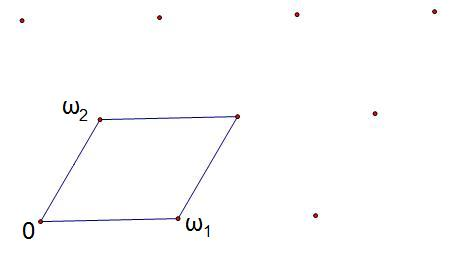
\includegraphics[scale=0.75]{ag-chapters/lattice2}\\
\caption{A lattice with fundamental parallelogram marked out.}
\end{figure}

We can identify the points in a fundamental parallelogram with the points of $\C/L$.

%MOVED TO INTRO
%Our goal is to show that there is a bijection between tori $\C/L$ and elliptic curves over the complex numbers $E/\C$, and in fact a group isomorphism between each torus and corresponding elliptic curve, with addition on the lattice corresponding to addition on the elliptic curve. 
%We will do this constructively: Given $L$, $E/\C\cong \C/L$. 
\begin{df}
An \textbf{elliptic function} is a complex function $f(z)$ for which there exists a lattice $L$ (the \textbf{period lattice} of $f$), such that the following hold:
\begin{enumerate}
\item
$f(z)$ is meromorphic, i.e. $f(z)$ is analytic everywhere
except for a discrete set of poles.
\item
$f(z)$ is periodic\footnote{also called {\it doubly periodic}, as this is equivalent to $f(z+\om_1)=f(z+\om_2)=f(z)$, when $L=[\om_1,\om_2]$} with respect to $L$:
\[
f(z+\om)=f(z)\text{ for all }\om\in L.
\]
\end{enumerate}
\end{df}
Recall that we say $f$ has a \textbf{pole} of order $k$ at $z_0$ if the equation
\[
\rc{f(z)}=(z-z_0)^kg(z)
\]
holds in a neighborhood of $z_0$, for some $g(z)$ analytic with $g(z_0)\ne 0$. 
For a fixed lattice $L$ the set of elliptic functions is a field, denoted $\C(L)$. Note that all constant functions are elliptic, so $\C\subeq \C(L)$.

\begin{df}
The \textbf{order} of an elliptic function is the number of poles it has in a fundamental parallelogram, counted with multiplicity.
\end{df}
%For example, $\wp$ has order 2 and $\wp'$ has order 3.
\begin{thm}\label{thm:elliptic-order}
For any nonzero elliptic function $f(z)$ the number of zeros of $f$ in any fundamental parallelogram is equal to its order.
\end{thm}
\begin{proof}
Pick a fundamental parallelogram $F$ so that $f(z)$ has no zeros or poles on $\partial F$ (the boundary of $F$). Orient the boundary counterclockwise. We use the following theorem from complex analysis, which is a consequence of Cauchy's integral formula.
\begin{thm}
Let $f$ be a meromorphic function and $F$ be a region whose boundary is a simple curve. Then
\[
\rc{2\pi i}\int_{\partial F} \fc{f'(z)}{f(z)}=\text{(number of zeros of $f$ in $F$)}-\text{(number of poles of $f$ in $F$)}.
\]
\end{thm}
\begin{proof}
See Ahlfors~\cite{Ah79}, Theorem 4.10.
\end{proof}
By periodicity the integral along opposite sides of $\partial F$ cancel each other out, because $F$ is the same on opposite sides but we're integrating in opposite directions.
%4.20 in Ahlfors, Complex Analysis
Hence
\[
\rc{2\pi i}\int_{\partial F} \fc{f'(z)}{f(z)}=0.
\]
The theorem then gives the result.
\end{proof}

\subsection{Eisenstein series}
Before we talk about the Weierstrass $\wp$-function, we talk about Eisenstein series, which will crop up during computation of $\wp$.
\begin{df}
Let $L$ be a lattice and $k>2$ be an integer.
The \textbf{Eisenstein series} for $L$ of weight $k\in \Z$ is
\[
G_k(L):=\sum_{\om\in L-\{0\}} \rc{\om^k}.
\]
\end{df}
\begin{rem}
This is a function of a {\it lattice}. We can also define the Eisenstein series as a function of a complex variable $z$ with $\textrm{Im} (z)>0$ by
\[
G_k(z):=G_k((1,z))=\sum_{(a,b)\in \Z^2-\{(0,0\}}\rc{(a+bz)^k}.
\]
Because it comes from function defined over a lattice, $G_k(z)$ has nice transformation properties. It is the basic example of a {\it modular form}. See Apostol,~\cite{Ap94}.
\end{rem}
\begin{rem}\label{rem:k-odd-zero}
Note that the Eisenstein series is identically 0 whenever $k$ is odd, because $\rc{\om^k}$ and $\rc{(-\om)^k}$ cancel out.
\end{rem}
\begin{lem}\label{lem:gk-conv}
$G_k$ converges absolutely for all $k>2$.
\end{lem}
\begin{proof}
The idea is that there are on the order of $n$ lattice points at distance between $n$ and $n+1$ from the origin, and they contribute at most $n\cdot \rc{n^k}=\rc{n^{k-1}}$ to the sum.

Let $\de$ be the minimum distance between points in $L$. Consider an annulus of radius $r$ and width $\fc{\de}2$.

\begin{figure}[h!] %Appear HERE no matter what.
\centering
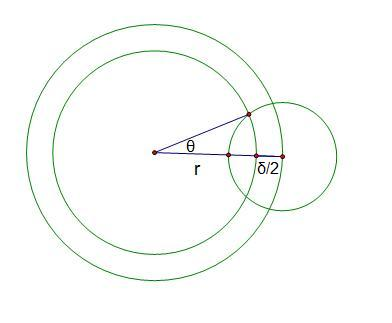
\includegraphics[scale=0.75]{ag-chapters/annulus2}\\
\end{figure}
The number of lattice points in $A$ is bounded by $c_{\de}r$ for some $c_{\de}\in \R$, because there is a minimum angle $\te$ between any two lattice points in $A$. Thus the number of lattice points in the annulus $\{ n\le |\om|<n+1\}$ is at most $cn$, for some constanct $c$. %($c_n\sim \fc{c_{\de}}{\de}$.) 
We get
\[
\sum_{\om\in L,\,|\om|\ge 1} \rc{|\om|^k}
\le
\sum_{n=1}^{\iy}
\fc{cn}{n^k}
=
c
\sum_{n=1}^{\iy}
\rc{n^{k-1}}
<\iy
\]
so $G_k(L)=\sum_{\om\in L,\,0<|\om|<1} \rc{\om^k}+\sum_{\om\in L,\,|\om|\ge 1} \rc{|\om|^k}$ converges absolutely.
\end{proof}
\subsection{The Weierstrass $\wp$-function}\label{sec:wp}
Now we define a special elliptic function.
\begin{df}
The \textbf{Weierstrass $\wp$-function} of $L$ is 
\[
\wp(z)=\wp(z;L)
=\rc{z^2}+\sum_{\om\in L-\{0\}} \pa{
\rc{(z-\om)^2}-\rc{\om^2}
}.
\]
\end{df}
We will write $\wp$ as a function of $z$, but keep in mind that it depends on $L$.
\begin{lem}
The sum in $\wp(z)$ converges absolutely and uniformly on all compact sets $\Om$ disjoint from $L$.
\end{lem}
\begin{proof}
We reduce to Lemma~\ref{lem:gk-conv} by bounding the summands using $\rc{|\om|^3}$.

Pick $r$ such that $|z|\le r$ for all $z\in \Om$. For all but finitely many $\om\in L$, we have $|\om|\ge 2r$. By the triangle inequality, $|\om-z|+|z|\ge |\om|$, so $|\om|\ge 2r$ implies
\begin{align*}
|\om-z|&\ge |\om|-|z|\ge \rc{2}|\om|\\
|2\om-z|&\le |2\om|+|-z|\le \fc 52 |\om|.
\end{align*}
Thus 
\[
\ab{
\rc{(z-\om)^2}
-
\rc{\om^2}
}
=
\ab{\fc{z(2\om-z)}{\om^2(z-\om)^2}}
\le
\fc{r\fc52|\om|}{|\om|^2(\rc2|\om|)^2}=\fc{10r}{|\om|^3}.
\]
But $\sum_{\om\in L-\{0\}}\rc{|\om|^3}$ converges by  Lemma~\ref{lem:gk-conv}. The last bound is independent of $z\in \Om$ (since we chose $r$ to work for all $z\in \Om$) so we have uniform convergence.
\end{proof}
The following properties are immediate.
\begin{cor}$\,$
\begin{enumerate}
\item
$\wp(z)$ is meromorphic. Its only poles are double poles at points in $L$.
\item
$\wp(z)$ is even: $\wp(z)=\wp(-z)$
\item
$\wp'(z)=-2\sum_{\om\in L} (z-\om)^{-3}$ is defined at all $z\nin L$. It is a memorphic odd function with poles of order 3 at each lattice point.
\end{enumerate}
\end{cor}
\begin{proof}
For the first item, note that a sum of meromorphic functions that converges absolutely is meromorphic. To see that $\wp(z)=\wp(-z)$ simply make the substitution $\om\mapsfrom -\om$ in the sum. Finally, since the sum converges uniformly to a meromorphic function, we can take the derivative inside the sum.
\end{proof}
The most important fact about $\wp$ is the following.
\begin{thm}
$\wp(z)$ is an elliptic function.
\end{thm}
\begin{proof}
We've already shown $\wp$ is meromorphic; it remains to show that $\wp(z+\om)=\wp(z)$ for all $\om\in L=[\om_1,\om_2]$. It suffices to show that
\[
\wp(z+\om_j)=\wp(z),\quad j=1,2.
\]
%keep subtract out \om_1,\om_2
Now $\wp'(z)$ is clearly periodic, so $\wp'(z+\om_j)=\wp'(z)$. Integrating gives
\[
\wp(z+\om_j)-\wp(z)=c_j.
\]
for some constant $c_j$ and for all $z\nin L$. To find $c_j$, take $z=\fc{\om_j}{2}$. We have
\[
\wp\pf{\om_j}2-\wp\pf{-\om_j}2=c_j.
\]
However, as $\wp$ is even, we get $c_j=0$, as needed.
\end{proof}
Note $\wp$ has order 2 and $\wp'$ has order 3, their only poles being the points of $L$.

In fact $\wp$ is the ``building block" of all elliptic functions, in the following sense.
\begin{thm}
The field of all elliptic function $\C(L)$ is generated by $\wp$ and $\wp'$:
\[
\C(L)=\C(\wp,\wp').
\]
\end{thm}
\begin{proof}
See Silverman \cite{Si86}, Theorem VI.3.2.
\end{proof}
%Think of $\wp$ as the ``universal" elliptic function. 
The definition of $\wp$ goes all the way back to Gauss because it shows up in elliptic integrals. To evaluate the integral one gets a differential equation, exactly the equation satisfied by $\wp$. Thus, $\wp$ was of interest long before anyone was interested in elliptic curves.

To compute with the Weierstrass $\wp$-function, we need to expand it in Laurent series.
\begin{thm}
The Laurent series expansion for $\wp(z)$ at 0 is
\[
\wp(z)=\rc{z^2}+\sum_{n=1}^{\iy} (2n+1)G_{2n+2}(L)z^{2n}.
\]
\end{thm}
\begin{proof}
For all $|x|<1$,
\[
\rc{(1-x)^2}=(1+x+x^2+\cdots )^2=\sum_{n=0}^{\iy} (n+1)x^n.
\]
Using this expansion, for $x=\fc zw$, $|x|<1$, 
\[
\rc{(z-\om)^2}-\rc{\om^2} =\rc{\om^2}
\pa{
\rc{(1-x)^2}-1
}=
\rc{\om^2}
\sum_{n=1}^{\iy}(n+1)x^n
=\sum_{n=1}^{\iy} \fc{(n+1)z^n}{\om^{n+2}}
\]
Summing over $\om$ and exchanging order of summation (which is okay by absolute convergence) gives
\begin{align*}
\wp(z)&=
\rc{z^2}+\sum_{\om\in L-\{0\}} \sum_{n=1}^{\iy}
\fc{(n+1)z^n}{\om^{n+2}}\\
&=\rc{z^2}+ \sum_{n=1}^{\iy} (n+1)G_{n+2}(L)z^n\\
&=\rc{z^2}+ \sum_{n=1}^{\iy} (2n+1)G_{2n+2}(L)z^{2n}.
\end{align*}
In the last step we noted that $\wp$ is even, so the coefficients of the odd terms are 0, and we can take the sum over just even integers $2n$. (Alternatively, Remark~\ref{rem:k-odd-zero} gives that the odd terms are 0.)
\end{proof}
\subsection{Lattices correspond to elliptic curves}\label{sec:corresp}
The key link between $\wp$ and elliptic curves is given by the following differential equation.
\begin{thm}
$\wp(z)$ satisfies
\begin{equation}\label{eq:wp-diffeq}
\wp'(z)^2=4\wp(z)^3-g_2(L)\wp(z)-g_3(L)
\end{equation}
where $g_2(L)=60G_4(L)$ and $g_3(L)=140G_6(L)$.
\end{thm}
If we let $y=\wp'(z)$ and $x=\wp(z)$ then this becomes the equation of an elliptic curve. (A simple substitution brings it into Weierstrass form.)
\begin{proof}
Write out the first few terms of the Laurent series for $\wp$ and differentiate. We compute the following.
\begin{align*}
\wp(z)&=\rc{z^2}+3G_4(L)z^2+5G_6(L)z^4+\cdots\\
\wp'(z)&=-\fc2{z^3}+6G_4(L)z+20G_6(L)z^3+\cdots\\
\wp(z)^3&=\rc{z^6}+\fc{9G_4(L)}{z^4}+15G_6(L)+\cdots\\
\wp'(z)^2&=\fc{4}{z^6}-\fc{24G_4(L)}{z^2}-80G_6(L)+\cdots 
\end{align*}
Now let $F(z)=\wp'(z)^2-4\wp(z)^3+60G_4(L)\wp(z)+140G_6(L)$. The negatives powers cancel and we have $F(0)=0$. Because $\wp,\wp'$ only has poles at points of $L$, this shows $F$ is analytic everywhere. Note $F$ is bounded because all values attained by $F$ are attained on a fundamental parallelogram, whose closure is compact. 
We now apply the following theorem from complex analysis.
\begin{thm}[Liouville's Theorem]
If $F$ is a bounded function analytic on all of $\C$, then $F$ is constant.
\end{thm}
By Liouville's Theorem, $F$ is constant, so $F=0$ identically.
\end{proof}
\begin{lem}\label{lem:p-2-torsion}
If $\om\nin L$ and $2\om\in L$ then $\wp'(\om)=0$.
\end{lem}
This is reminiscent of the fact that for elliptic curves, the 2-torsion points are the points with $y=0$.
% rule for 2-torsion for elliptic curves: $w$ corresponds to a point not equal to $\iy$, that is $\iy$ when doubled; this says $y=0$ for such a point.
\begin{proof}
Since $\wp'$ is periodic and odd, we have
\[
\wp'(\om)=\wp'(\om-2\om)=\wp'(-\om)=-\wp'(\om)=0.
\]
\end{proof}
%compute directly by approximate laurent series approximation.

Equation~\eqref{eq:wp-diffeq} shows looks like the equation of an elliptic curve. However, in order for it to actually correspond to an elliptic curve we need to show that the discriminant is nonzero. Define the \textbf{discriminant} of a lattice to be
\[
\De(L)=g_2(L)^3-27g_3(L)^2.
\]
Note that this equals $2^{12}\De(E)$ where $E$ is the elliptic curve $y^2=4x^3-g_2(L)x-g_3(L)$ corresponding to $L$.
\begin{lem}
The discriminant $\De(L)$ is nonzero.
\end{lem}
\begin{proof}
Let $L=[\om_1,\om_2]$. Let
\[
r_1=\fc{\om_1}2,\quad r_2=\fc{\om_2}2,\quad r_3=\fc{\om_1+\om_2}2.
\]
Then $2r_j\in L$ for $j=1,2,3$. So
$\wp'(r_j)=0$ by Lemma~\ref{lem:p-2-torsion}. Hence by Theorem~\ref{eq:wp-diffeq}, $\wp(r_1),\wp(r_2),\wp(r_3)$ are the zeros of the cubic $p(x)=4x^3-g_2(L)x-g_3(L)$. Now the discriminant $\De(L)$ is $\rc{16}$th of the discriminant of $p=x^3-4g_2x-16g_3$:
\[
\De(L)=\rc{16}\De(p)=\prod_{\al,\be \text{ distinct roots of }p}(\al-\be).
\] 
Thus it suffices to show that the $\wp(r_j)$ are distinct.

Let $f(z)=\wp(z)-\wp(r_1)$. Then $f(z)$ is an elliptic function of order 2 (its poles are the poles of $\wp$), so it has 2 zeros by Theorem~\ref{thm:elliptic-order}. Now $r_1$ is a double zero because $\wp'(r_1)=0$ by Lemma~\ref{lem:p-2-torsion}. Thus $f$ can have no more zeros, showing
\[
\wp(r_2)\ne \wp(r_1)\text{ and }\wp(r_3)\ne \wp(r_1).
\]
Similarly $\wp(r_2)\ne \wp(r_3)$, as needed.
\end{proof}
We've now shown that $\Phi(z)=(\wp(z),\wp'(z))$ gives a map from $\C/L$ to the elliptic curve $y^2=4x^3-g_2(L)x-g_3(L)$. We still have to show this is a bijection and a group homomorphism. We will do this in the next lecture.
\section{Lecture 19: 4/24}
\begin{df}
\begin{enumerate}
\item
A complex function $f(z)$ is (complex) \textbf{analytic} (or \textbf{holomorphic}) at $z_0$ if the derivative $f(z)=\lim_{h\to 0} \fc{f(z+h)-f(z)}{h}$ exists in some neighborhood of $z_0$.
\item
$f(z)$ is \textbf{meromorphic} if it is analytic everywhere except for a discrete set of poles.
\item
$f(z)$ has a \textbf{zero} of order (multiplicity) $k$ at $z_0$ if $f(z)=(z-z_0)^kg(z)$ for some $g(z)$ analytic at $z_0$ with $g(z_0)\ne 0$. $f(z)$ has a \textbf{pole} of order $k$ at $z_0$ if $\rc{f(z)}$ has a zero of order $k$ at $z_0$.
\end{enumerate}
\end{df}

Fact: in any fundamental region for $L$, an elliptic function $f$ has an equal number of zeros and poles, called the order of $f$.

We want to show there is a one-to-one correspondence between  complex tori and elliptic curve, compatible with group operations.
Given elliptic curve, show how to get tori out of it.

\begin{thm}
Let $L$ be a lattice and $E/\C$ be the elliptic curve
\[
y^2=4x^3g_2(L)x-g_3(L).
\]
(Note: setting $A=-\fc{g_2}4$ and $B=-\fc{y_2}{3}$ gives $-16(4A^3+27B^2)=\De(L)\ne 0$.)

The map $\Phi:\C/L\to E(\C)$ defined by 
\[\Phi(z)=(\wp(z),\wp'(z))\]
and $\Phi(0)=\iy$ is a group isomorphism.
\end{thm}
Adding on the lattice the the same thing as adding on the elliptic curve (even though adding on elliptic curve appears to be more complicated).
%could have done easier if we had done this earlier. For example, proving associativity.
%If can embed things in $\C$. Still good do things algebraically.
%a lot of proofs of facts in char 0 bc this simplifies a lot of proofs
\begin{proof}
First we show surjectivity. Let $(x_0,y_0)\in E(\C)$. The elliptic function $\wp(z)-x_0$ has order 2, so it has 2 zeros $\pm z_0\in \C/L$, with $x_0=\wp(z_0)$ and $y_0=\pm\wp'(z)_0$.

Next we show injectivity. Suppose $z_1,z_2\in \C/L$, $z\ne z_2$ nonzero points. Suppose $\wp(z_1)=\wp(z_2)$ and $\wp'(z_1)=\wp'(z_2)$. We can assume $z_1,z_2\ne 0$ because 0 is the only point sent to $\iy$. If $2z_1\in L$, then $\wp'(z_1)=0$. Hence $z_1$ is a double root of $\wp(z)-\wp(z_1)$. Since this is an elliptic function of order 2, it is the only root. Hence $\wp(z_2)\ne \wp(z_1)$. Otherwise, if $\wp(z_2)=\wp(z_1)$ then $z_2=-z_1$. But then $\wp'(z_0)=\wp'(-z_1)\ne \wp(z_1)$ since the derivative was odd. Contradiction.

%The elliptic function $\wp(z)-\wp(z_0)$ has 2 zeros $\pm z$ so $z_2=\pm z_1$ and $\wp'(z_2)=\wp'(z_1)$ and $z_2=z_2$.
%%If $\wp'(z_1)=0$,
%Or $z_1=-z_2$, $\wp'(z_1)=0$. Then $2z_1\equiv 2z_2$, and $z_1\equiv z_2$...
Now we show the map is a homomorphism. By construction it preserves the identity and inverses, because $\phi(-z)=(\wp(-z),\wp'(-z))=(\wp(z),-\wp'(z))=-\phi(z)$. Let $z_1,z_2\in \C/L$ be nonzero. (It handles addition by 0 correctly.) First assume $z_1\ne z_2$. Let 
\begin{align*}
P_1&=(x_1,y_1)=(\wp(z_1),\wp'(z_1))\\
P_2&=(x_2,y_2)=(\wp(z_2),\wp'(z_2)).
\end{align*}
\end{proof}
Let $y=ax+b$ be the line through $P_1$ and $P_2$ and let $(x_3,y_3)$ be the third point on the line that intersects $E/\C$, so that $P_1+P_2+P_3=O$. By the group law on $E/\C$, (the same formula we know and love, just with a $\rc4$ factor)
\begin{align*}
x_3&=\rc 4\pf{y_2-y_1}{x_2-x_1}^2-x_1-x_2\\
&=\rc4 \pf{\wp'(z_2)-\wp'(z_1)}{\wp(z_2)-\wp(z_1)}-\wp(z_1)-\wp(z_2).
\end{align*}
Consider the function $\ell(z)=-\wp'(z)+a\wp(z)+b$. This is a sum of elliptic functions of order 3 ($\wp'(z)$ has a pole where $\wp$ has a zero) so $\ell(z)$ has 3 zeros, 2 of which are $z_1$ and $z_2$. Let $z_3$ be the third zero. From Cauchy's Residue Theorem,
\[
\rc{2\pi i}\int_{\partial F} z\fc{\ell'(z)}{\ell(z)}
=\sum_{w\in F} \ord_w(\ell)w=z_1+z_2+z_3-3\cdot 0.
\]
%%%%%%%%%%%%%%
\begin{proof}
Label the edges of the fundamental parallelogram as follows.
\[
\xymatrix{
& \al+\omega_2 \ar[rr]^{C_2} & & \al+\omega_1+\omega_2\ar[ld]^{C_3} \\
\al\ar[ur]^{C_1} & &\al+\omega_1 \ar[ll]^{C_4}&
}
\]
We calculate $\int_{\partial P} \frac{zf'(z)}{f(z)}\,dz$ in two ways.

\textbf{Way 1:} 
\[
\int_{\partial P} \frac{zf'(z)}{f(z)} \,dz=\ba{
\int_{C_1} \frac{zf'(z)}{f(z)}\,dz
+\int_{C_3} \frac{zf'(z)}{f(z)}\,dz
}
+\ba{
\int_{C_2} \frac{zf'(z)}{f(z)}\,dz
+\int_{C_4} \frac{zf'(z)}{f(z)}\,dz
}.
\]
Noting that $C_3$ is just $C_1$ shifted by $\omega_1$ and reversed, and that $C_2$ is just $C_4$ shifted by $\omega_2$ and reversed, this equals
\[
\int_{\partial P} \frac{zf'(z)}{f(z)} \,dz=
\int_{C_1} \ba{\frac{zf'(z)}{f(z)}
-\frac{(z+\omega_1)f'(z+\omega_1)}{f(z+\omega_1 )}
}\,dz
+
\int_{C_4} \ba{\frac{zf'(z)}{f(z)}- \frac{(z+\omega_2)f'(z+\omega_2)}{f(z+\omega_2)}
}\,dz.
\]
Since $f$ is elliptic, $f(z)=f(z+\omega_1)=f(z+\omega_2)$, giving
\[
\int_{\partial P} \frac{zf'(z)}{f(z)} \,dz=
-\omega_1\int_{C_1} \frac{f'(z)}{f(z)} \,dz-\omega_2\int_{C_4} \frac{f'(z)}{f(z)}\,dz.
\]
Now $\ln(f(z))$ can be defined in a neighborhood around $C_1$ and $C_4$, since $f$ has no poles or zeros on $\partial P$. Since $f(\al)=f(\al+\omega_1)=f(\al+\omega_2)$, we have $\ln(f(\al+\omega_1))-\ln(f(\al))=2\pi i c_1$ and $\ln(f(\al))-\ln(f(\al+\omega_2))=2\pi i c_2$ for some integers $c_1$ and $c_2$. But these equal the above integrals by definition of $\ln f(z)$, so
\begin{equation}\label{p1-1-1}
\int_{\partial P} \frac{zf'(z)}{f(z)} \,dz=
-2\pi i(\omega_1 c_1+\omega_2 c_2).
\end{equation}

\textbf{Way 2:}
Note $\Res_a \frac{f'(z)}{f(z)}=\ord_a f$ so $\Res_a \frac{zf'(z)}{f(z)}=a \ord_a f$. Letting $a_k$ be the poles and zeros of $f$ in $P$, we get by Cauchy's Theorem that
\begin{equation}\label{p1-1-2}
\int_{\partial P} \frac{zf'(z)}{f(z)}=2\pi i\sum_{k} \Res_{a_k} \frac{f'(z)}{f(z)}=2\pi i \sum_{k}m_k a_k.
\end{equation}
Equating~(\ref{p1-1-1}) and~(\ref{p1-1-2}) give
\[
\sum_{k}m_ka_k=-\omega_1c_1-\omega_2c_2\equiv 0\pmod{\La}.
\]
%%%%%%%%%%
Last fact from complex analysis: The winding number of a closed curve $\ga$ about $a$, defined as
\[
W(\ga,a):=\rc{2\pi i}\int_{\ga}\fc{dz}{z-a},
\]
is an integer. It counts how many times the curve goes around $a$. Let $f(z)=\fc{\ell'(z)}{\ell(z)}$ be an elliptic function, so $f(0)=f(\om_2)=f(\om_1)$. Let $z=f(t\om_j)$, $0\le t\le 1$. This parametrizes a closed curve, so
\[
\rc{2\pi i}\int_0^{\om_2}f(z)\,dz\in \Z\implies z_1+z_2+z_3=c\om_1+d\om_2\equiv 0\pmod L.
\]
Starting with 3 points that sum to 0, their images on the torus sum to 0. %This takes care of most of it.
This imples 
\[
\wp(z_1+z_2)=\wp(-z_3)=\wp(z_3)=x_3,
\]
so $\Phi(z_1+z_2)=\pm(\Phi(z_1)+\Phi(z_2))$. Suppose $\Phi(z_1+z_2)=-(\Phi(z_1)+\Phi(z_2))$. Then $\Phi(z_1+z_2)=\Phi(-x_1)+\Phi(-x_2)$ and $\Phi(z_1)+\Phi(z_2)=-\Phi(z_1+z_2)$. Then $\Phi(z_1)=-\Phi(z_1+z_2)-\Phi(z_2)=\pm \Phi(z_1+2z_2)$. This implies $\wp(z_1)=\wp(z-1+2z_2)$. Either $2z_2\in L$ or $2z_2=-z_1$. Thus
\[
\Phi(z_1+z)=\Phi(z_1)+\Phi(z)
\]
for all but finitely many $z$ ($z=z_1$, $2z\in L$, and $2z_2=-z_1$. By continuity $\Phi(z_1+z)=\Phi(z_2+z)$ for all $z$.\end{proof}
\begin{df}
Define the \textbf{$j$-invariant} of a lattice by
\[
j(L)=1728\fc{g_2(L)^3}{\De(L)}=1728\fc{g_2(L)^3}{g_2(L)^3-27g_3(L)^2}.
\]
(Recall $\De(L)\ne 0$.)

If $E$ is an elliptic curve $y^2=x^3+Ax+B$ then let $g_2=-4A$ and $g_3=-4B$ (so $E$ is equivalent to $y^2=4x^3-g_2x-g_3$). Then define the discriminant and $j$-invariant to be
\begin{align*}
\De(E)&=g_2^3-27g_3^2=(-4A)^3-27(-4B)^2=-16(4A^3+27B^2)\\
j(E)&=\fc{1728}{(-4A)^3}{-16(4A^3+27B^2)}=1728\fc{4A^3}{4A^3+27B^2}.
\end{align*}
\end{df}
Spend next 2 lectures understanding why we care about this thing.

\begin{df}
Lattice $L$ and $L'$ are \textbf{homothetic} if $L'=\la L$ for some $\la\in \C^{\times}$.
%give rise to same tori.
\end{df}
The $j$-invariant allows us to classify lattices up to isomorphism (homothetic), and hence elliptic curves over $\C$ (or algebraic closed fields of char 0).
Collapse two numbers into 1. Depends on $\om_1$ and $\om_2$, $g_2$ and $g_3$, but in fact parameterized by single number $j$-invariant. 

\begin{thm}
$L$ and $L'$ are homothetic iff $j(L)=(L')$.
\end{thm}
\begin{proof}
Let $L'=\la L$ and $\la\in\C^{\times}$. Then
\begin{align*}
g_2(L')&=60\sum_{\om\in L-\{0\}}\rc{\om^4} = 60\sum_{\om\in L-\{0\}} \rc{(\la \om)^4} =\la^{-4}g_2(L)\\
g_3(L')&=\la^{-6}g_3(L).
\end{align*}
So
\[
g(L')=1728\fc{\la^{-12}}{\la^{-12}g_2(L)^3-27\la^{-12}g_3(L)^2}=j(L).
\]

For the reverse direction, suppose $j(L)=j(L')$. Let
\begin{align*}
g_2&=g_2(L)&
g_3&=g_3(L)\\
g_2'&=g_2(L')&
g_3'&=g_3(L')
\end{align*}
We claim that there exists $\la\in \C^{\times}$ such that $g_2'=\la^{-4}g_2$ and $g_3'=\la^{-6}g_3$.
Proof: consider 3 cases.
\begin{enumerate}
\item
$g_2'=0$: Then $g_2=0$ so pick $\la$ so $\la^6\ga_3'=\ga_3$.
\item
$g_3'=0$: Then $j(L')=j(L)=1728$ so $g_3=0$ and we can pick $\la$ such that $\la^4g_2'=g_2$.
\item
If $g_2',g_3'\ne 0$ then pick $\la$ such that $\la^4g_2'=g_2$. Then
\[
\fc{j(L)}{1728}=\fc{g_2^3}{g_2^3-27g_3^2}=\fc{\la^{-2}g_2^3}{\la^{-12}g_2^3-27{g_3'}^2}=\fc{j(L')}{1728}.
\]
We have
\begin{align*}
\la^{-12}g_2^3-27g_3'^2&=\la^{-12} g_2^3-27\la^{-12}g_3^2\\
\la^{12}g_3'^2&=g_3^2\\
\la^6g_3'&=\pm g_3.
\end{align*}
Replace $\la$ by $i\la$ if negative so $\la^6g_3'=g_3$. End proof of claim.

Recall that $\wp'(z)^2=4\wp(z)^3-g_2\wp(z)-g_3$. Differentiating,
\begin{align}
\nonumber
2\wp'(z)\wp''(z)&=12\wp(z)^2\wp'(z)-g_2\wp'(z)\\
\llabel{eq:wp''}
\wp''(z)&=6\wp(z)^2-\fc{g_2}2.
\end{align}
We have $\wp(z)=\rc{z^2}+\sum_{n=1}^{\iy} (2n+1)G_{2n+2}z^{2n}=\rc{z^2}+\sum_{n=1}^{\iy}a_nz^{2n}$. Then $a_1=\rc{20}g_2$ and $a_2=\rc{28}g_3$. ($g_2=60G_4$, $g_3=140G_6$.) The $z^{2n}$ term in~(\ref{eq:wp''}) for $n>2$ is
\[
(2n+2)(2n+1)a_{n+1}=6\pa{
\sum_{k=1}^{n-1} a_ka_{n-k} +2a_{n+1}
}.
\]
Thus we can compute all $a_n$ from $a_1$ and $a_2$. So $g_2$ and $g_3$ uniquely determine $\wp(z)$. Now consider $L'$ and $\la L$. We have
\begin{align*}
g_2(L')&=\la^{-4}g_2(L)=g_2(\la L)\\
g_3(L')&=\la^{-6}g_3(L)=g_3(\la L)\\
\wp(z;L')&=\wp(z;\la L)\implies & L'=\la L.
\end{align*}
\end{enumerate}
\end{proof}
$j(L)$ classifies lattices up to homothety. $j(E)$ classifies elliptic curves up to isomorphism over $\ol K$. $j(E)=j(E')$ iff $E/\ol K\cong E'/\ol K$. See Silverman III.1.4. Not true for non-algebraically closed fields, ex. quadratic twists.
\subsection{$\SL_2(\Z)$}
\begin{df}
$\SL_2(\Z)$ is the group of $2\times 2$ integer matrices with determinant 1.
\[
\SL_2(\Z):=\set{\matt abcd}{a,b,c,d\in \Z, \, ad-bc=1}.
\]
Define $\PSL_2(\Z)=\SL_2(\Z)/\{\pm 1\}$.
Define the following subgroups:
\begin{align*}
\Ga(N)&=\set{M\in \SL_2(\Z)}{M\equiv \matt 1001\pmod{N}}\\
\Ga_1(N)&=\set{M\in \SL_2(\Z)}{M\equiv \matt 1*01\pmod{N}}\\
\Ga_0(N)&=\set{M\in \SL_2(\Z)}{M\equiv \matt **0* \pmod{N}}.
\end{align*}
Any subgroup of $\SL_2(\Z)$ containing $\Ga(N)$ for some $N$ is called a \textbf{congruence subgroup}.
\end{df}
\begin{df}
%The fractional linear transformation transformation associated to $\matt abcd$ is
%\[
%z\mapsto \frac{az+b}{cz+d}.
%\]
%\end{df}
%Note that the map $\matt abcd \mapsto \frac{az+b}{cz+d}$ is a group isomorphism between $\PSL_2(\Z)$ and the group of fractional linear transformations. We often use a matrix to denote the fractional linear transformation.
$\SL_2(\Z)$ acts on the upper half plane $\cal H$ via fractional linear transformations
\[
\matt abcd z=\frac{az+b}{cz+d}.%drew uses tau.
\]
\end{df}
It's easy to check this is in the upper half-plane.

\begin{df}
A \textbf{fundamental domain} of $M$ under a group action $G$ is a subset $F$ of $M$ such that for every $\tau\in \cal H$ there exists $\tau'\in F$ such that $\ga(\tau)=\tau'$. ADD TOPOLOGICAL CONDITION.
\end{df}
\begin{lem}
The region
\[
F=\set{z\in \cal H}{\Re(z)\in [-\rc 2,\rc 2),\,|z|\ge 1 \text{ for }\Re(z)<0,\,|z|>1 \text{ for }\Re(z)>0}
\]
is a fundamental domain for $\cal H/\SL_2(\Z)$.
\end{lem}
\begin{proof}
For any $\tau\in \cal H$, 
\[
\Im(\ga\tau)=\fc{\Im(\tau)}{|c\tau+d|^2}>\im(\tau)
\]
for only finitely many pairs $(c,d)$. We can pick $\ga\in \SL_2(\Z)$ such that $\im(\ga\tau)$ is as large as possible. Now multiply $\ga\tau$ by $\ga'=\smatt 1a01$ so $\tau'=\ga'\ga\tau$ has $\Re(\tau')=[-\rc 2,\rc2)$. Claim: $|\tau'|\ge 1$. If not then $\Im(\tau')<\Im\pa{-\rc{\tau}}$, but then $\Im\pa{\smatt 01{-1}0 \ga'\ga\tau}>\Im(\ga \tau)$.

Finally, if $\Re(\tau')>0$ and $|\tau|=1$ then replace $\tau'$ by $-\rc{\tau'}$.

We now prove uniqueness. It suffices to show no two elements of $F$ are $\SL_2(\Z)$-equivalent. Suppose $\tau_1\ne \tau_2$ are in $F$ and $\tau_2=\ga\tau_1$. Their imaginary parts have to be different (otherwise the matrix relating them would be $\smatt1j01$ for some $j$, and they can't be in the same strip), so assume $\Im \tau_2>\Im \tau_1$. Letting $\ga=\smatt abcd$, we have
\[
\Im \tau_2=\fc{\Im \tau_1}{|c\tau_1+d|^2}
\]
where $|c\tau_1+d|^2<1$. Then
\begin{align*}
1>|c\tau_1+d|^2=(c\tau_1+d)(c\ol{\tau_1}+d)
&= c^2|\tau_1|+d^2+2cd\Re \tau_1\\
&\ge c^2+d^2-cd.
\end{align*}
This has no integer solutions except $(c,d)=(0,0)$, so we get a contradiction.
\end{proof}
%(matrices invertible. if two different matrices mapping, )
\section{Lecture 20: 4/26}
Define the $j$-function $\cal H\to \C$ by $j(\tau)=j([1,\tau])$. Similarly define $g_2(\tau)$, $g_3(\tau)$, and $\De(\tau)$.

Note we get all lattices up to homothety in this way because $[\om_1,\om_2]=\om_1\ba{1,\fc{\om_2}{\om_1}}=\om_1[1,\tau]$.

\begin{thm}[$j$ is a modular function of weight 0]
The $j$ function satisfies the following.
\begin{enumerate}
\item
$j(\tau)=j(\ga\tau)$ for all $\ga\in \SL_2(\Z)$ (i.e. $j$ is $\SL_2(\Z)$-invariant).
\item
$j(\tau)$ is holomorphic on $\cal H$>
\item
The restriction $j:F\to \C$ is a bijection. In particular, $j$ is surjective.
\end{enumerate}
\end{thm}
This will show every elliptic curve comes from some torus.
\begin{proof}
Item 1 is immediate from the fact that $\ga$ sends a lattice to a homothetic lattice.

For item 2, note
\[
j(\tau)=1728\fc{g_2(\tau)^3}{\De(\tau)},\quad \De(\tau)\ne 0\text{ for all }\tau\in \cal H.
\]
Now $g_2(\tau)$ is defined everywhere so $j(\tau)$ is. We just need to show $g_2(\tau)$ and $g_3(\tau)$ are holomorphic.

We use the following.
\begin{thm}[Weierstrass, Ahlfors Theorem 5.1]
If $f(z)$ is the limit of a sequence of analytic functions $f_n(z)$ that converges uniformly on every compact subset of some region $U$. Then $f$ is analytic on $U$.
%Weierstrass function meromorphic.
\end{thm}
Let $\Ga$ be a compact subset of $\cal H$. Then there exists $\de>0$ such that $\Im(\tau)\ge \de>0$ for every $\tau\in \Om$ ($\de<1$). Let $\tau'=\tau+a$ with $a\in \Z$, so $\Re(\tau)\in [-\rc 2,\rc 2]$. Now $G_4(L)$ converges absolutely: $g_2(\tau')=g_2(\tau)=g_2(\tau)$. We have
\[
g_2(\tau')=60\sum_{\om\in L-\{0\}} \rc{\om^4}=60\sum_{(m,n)\in \Z^2-\{(0,0)\}} \rc{(m+n\tau')^4}.
\]
By exercise 1.13 in Cox, $|m+n\tau'|\ge \fc{\de}{2}\sqrt{m^2+n^2}$. %go out far, tail negligible.
Let $f_N(z')=60 \sum_{m,n,|m+n\tau|\le N}'\rc{(m+n\tau)^4}$. For all $\ep>0$ and every $N\ge N_0$ there exists $z'$ so that $|f_N(z')-g_2(\tau')|<\ep$. Thus $f_N\to g_N$ unifomly. ($g_2$ is periodic, so this is true everywhere.) So $g_2$ is analytic, and similarly, so is $g_3$. So $j$ is holomorphic on $\cal H$.

For item 3, we have already shown injectivity. Now
\begin{align*}
g_2(\tau)&=60\sum_{m,n} \rc{(m+n\tau)^4}
=60\pa{2\sum_{m=1}^{\iy} \rc{m^4}+\sum_{m,n,n\ne 0}\rc{(m+n\tau)^4}}.\\
\lim_{\Im \tau \to 0} g_2(\tau)&=120\ze(4) = 120\fc{\pi^4}{90} =120\fc{\pi^4}{90}=\fc 43\pi^4\\
\lim_{\Im \tau\to \iy} g_3(\tau)&=280\ze(6) =280 \fc{\pi^6}{945}=\fc{8}{27}\pi^6\\
\lim_{\Im \tau\to \iy} \pa{\fc 43\pi^4}^3-27\pa{\fc 8{27}\pi^6}^2&=\fc{64}{27}\pi^{12}-\fc{64}{27}\pi^{12}=0.
\end{align*}
The $j$ function is holomorphic and not constant on $\cal H$. So its image is an open subset of $\C$. We will show that the image is also closed, hence equal to $\C$. Let $j(\tau_n)$ be a sequence of points in $\C$ convergine to some $w\in \C$. We may assume $\tau_n\in F$ and $\Im \tau_n$ must be bounded because $j(\tau)\to \iy$ as $\Im\tau\to \iy$. Therefore the $\tau_n$ all lie in a compact subset $\ol F$. So there is a subsequence of $\tau_n$ converging to some $\tau$. By continuity $j(\tau)=w$ so its image is closed.
\end{proof}
\begin{cor}[Uniformization theorem]
For every elliptic curve $E/\C$ there is a lattice $L=[1,\tau]$ such that $\C/L\cong E(\C)$. 
\end{cor}
\begin{proof}
$j$ is surjective so there exists $z\in \cal H$ such that $j(\tau)=j(E)$ amd the lattice $[1,\tau]$ homothetic to a lattice $L'$ for which $g_2(L')=-4A$, $g_3(L')=-4B$ where $E:y^2=x^3+Ax+B$.
\end{proof}
We've shown there is a one-to-one correspondence between lattices corresponding to complex tori and elliptic curves over $\C$.
\begin{thm}
For every $j\in K$ there exists an elliptic curve $E/K$ with $j$-invariant $j(E)$.
\end{thm}
\begin{proof}
Assume $\chr(k)\ne 2,3$ (but it's true in general). For $j=0$ let $y^2=x^3+1$. For $j=1728$ let $E:y^2=x^3+x$. For $j\ne 0,1728$, let
\begin{align*}
A&=3j(1728-j)\\
B&=2j(1728-j)^2.
\end{align*}
\end{proof}
\begin{thm}
Two elliptic curves $E/K$ and $E'/K$ defined by $y^2=x^3+Ax+B$ and $y^2=x^3+Ax'+B$ are isomorphic iff $A'=\mu^4A$ and $B'=\mu^6B$ for some $\mu\in \ol K^{\times}$.
\end{thm}
\begin{proof}
An isomorphism $\phi$ must be an isogeny of degree 1, because $\phi\phi^{-1}=1$ gives $\deg(\phi)\deg(\phi^{-1})=1$. %don't have to prove dual isogeny exists.
Let $\phi=(r_1(x),r_2(x)y)$ be the isomorphism $E'\to E$. Now $\ker\phi=\{0\}$ so $r_1$ and $r_2$ are polynomials. Now $\deg(\phi)=1$ implies $r_1(x)=ax+b$ for $a,b\in \ol K$ and $a\ne 0$. We get
\begin{align*}
r_2^2 y^2 &= (ax+b)^3+A(ax+b)+B\\
r_2(x)^2(x^3+A'x+B')&= (ax+b)^3 +A(ax+b)+B.
\end{align*}
Comparing coefficients we get $B=C$, $b=0$, $c^2=a^3$, $c=\mu^6$, $a\in \mu^4$ for some $\mu\in \ol K^{\times}$.Thus $A'=\mu^4A$ and $B'=\mu^6B$. Conversely, $\phi=(\mu^4x,\mu^6y)$ is an isomorphism.
%$\Q$ infinitely many quad twists of curve not iso over \Q
\end{proof}
Our next big theorem! We relate maps between lattices and maps between elliptic curves.
\begin{thm}
Let $L$ be a lattice and $E/\C$ be an elliptic curve. Let $\Phi:\C/L\xra{\cong}E(\C)$ be the natural isomorphism. Then the following are equivalent.
\begin{enumerate}
\item
$\al L\subeq L$.
\item
$\wp(\al z)=\fc{A(\wp(z))}{B(\wp(z))}$ for $A,B\in \C[X]$.
\item
There exists $\phi \in \End(E)$ such that the diagram
\[
\xymatrix{
\C/L \ar[r]^{\Phi}\ar[d] \ar[r]^{\Phi}& E(\C)\ar[d]^{\Phi}\\
\C/L \ar[r]^{\Phi} & E(\C).
}
\]
commutes.
\end{enumerate}
Conversely, every  $\phi\in \End(E)$ gives rise to an $\al$ satisfying (i) to (iii). This gives a ring isomorphism
\[
\End(E)\cong \set{\al}{\al L\subeq L}.
\]
If (i) to (ii) hold then
\[
\deg(A)=\deg(B+1)=\nm(\al)=N(\phi).
\]
\end{thm}
%If $\al$ satisfies (i) then it gives rise to an endomorphism.

This is why we call complex multiplication. CM elliptic curves have endomorphisms corresponding to $\al\in \C-\R$ such that $\al L\subeq L$.
\begin{proof}
$(i)\implies (ii)$: Let $\om\in L$. Then
\begin{equation}\label{eq:p(az)}
\wp(\al(z+w))=\wp(\al z+\al w)=\wp(\al z)
\end{equation}
since $\al L\subeq L$. Thus $\wp(\al z)$ is periodic with respect to $L$. Now $\wp(\al z)$ is clearly meromorphic (as $\wp$ is), hence an elliptic function for $L$. Thus $\wp(\al z)$ is an even function and therefore a rational function of $\wp(z)$ (by a lemma to be proved).

$(ii)\implies (i)$: We have $B(\wp(z))\wp(\al z)=A(\wp(z))$. $\wp(z)$ and $\wp(\al z)$ both have a double pole at 0, so $\deg(A)=\deg(B)+1$. If $\om\in L$ then $\wp(\al z)$ has a pole at $\om$ by~(\ref{eq:p(az)}) and thus $\wp(z)$ has a pole at $\al \om$, so $\al L\subeq L$.

$(ii)\implies (iii)$: Let $\phi$ be the rational map $\pa{\fc{A(x)}{B(x)},\fc{C(x)}{D(x)}y}$, where $A$ and $B$ are as in (ii) and 
\[
\wp'(\al z)=\fc{C(\wp(z))}{D(\wp(z))}\wp'(z).
\] 
Hence $\phi$ gives an endomorphism. Then $\phi$ is an endomorphism (note $(\wp(\al z),\wp'(\al z))$ is on $E(\C)$ because it is $\Phi(\al z)$). Then
\begin{align*}
\phi(\Phi(z))&= \phi(\wp(z),\wp'(z)) =\pa{\fc{A(\wp(z))}{B(\wp(z))} \wp(z)}\\
&=(\wp(\al z),\wp'(\al z))=\Phi(\al z).
%go around diagram 1 way
%go around other way
\end{align*}

(iii)$\implies (ii)$: Let $\phi\in \End(E)$ satisfying (iii). Then $\om\in L$ so $\phi(\Phi(\om))=0=\Phi(\al \om)$, giving $\al\om \in L$ and $\al L\subeq L$.

Let $\phi\in \End(E)$. The map $\ol{\phi}(z)=\Phi^{-1}(\phi(\Phi(z)))$ is an endomorphism of $L$. We may assume $\ol{\phi}(0)=0$ and in some neighborhood of 0, 
\[
\ol{\phi}(z_1+z_2)=\ol{\phi}(z_1)+\ol{\phi}(z_2)
\]
over $\C$. Then
\[
\ol{\phi}'(z)=\lim_{h\to 0}\fc{\ol{\phi}(z+h)-\ol{\phi}(z)}{h}
=\lim_{h\to 0}\fc{\ol{\phi}(h)-\ol{\phi}(0)}h = \ol{\phi}'(0)=\al\in \C
\]
for some $\al$, so $\ol{\phi}(z)=\al z$ for all $z\in U$.

For any $z\in \C$, let $n\in \Z$ be such that $\fc{z}{n}\in U$. Then $\ol{\phi}(z)=n\ol{\phi}\pf zn=n\pf{\al z}{n}=\al z$ modulo $L$ so $\ol{\phi}(L)\subeq L$ and $\al L\subeq L$.

Let $\phi_1,\phi_2\in \End(E)$ with corresponding $\al_1,\al_2\in \C$. It's clear that $\phi_1+\phi_2$ corresponds to $\al_1+\al_2$, by linearity of the derivative. Then
\begin{align*}
\ol{\phi_1\cdot \phi_2}&=\ol{\phi_1}\circ \ol{\phi_2}\\
(\ol{\phi_1}\circ \ol{\phi_2})'(0)&= \ol{\phi_1}'(\ol{\phi_2}(0))\ol{\phi_2}'(0)=\ol{\phi_1}'(0)\ol{\phi_2}'(0)=\al_1\al_2.
\end{align*}
Thus there is a surjective ring homomorphism $\End(E)\tra \set{\al\in \C}{\al L\subeq L}$. Only the zero endomorphism has $\al=0$. So it is injective and hence an isomorphism.

It follows that $\al$ and $\phi$ have some characteristic polynomial, in particular $N(\al)=N(\phi)$ and $N(\phi)=\deg(\phi)=\deg A$.
\end{proof}
\begin{lem}
Let $f(z)$ be an even elliptic function for $L$. Then $f(z)$ can be written as a rational function of $\wp(z)$.
\end{lem}
\begin{proof}
\begin{enumerate}
\item
%We prove this by induction on the order of
If $f(z)$ is holomorphic on $\C-L$ then it has a Laurent expansion at $z=0$. Write
\[
f(z)=\sum_{k=-n}^{\iy} a_{2k} z^{2k}
\]
where $2n$ is the order of $f$. If $n>0$ then $(f(z)-a_{2n} \wp(z)^n)$ has order at most $2n-2$. Repeat (induct). There exists $A\in \C[X]$ of degree $n$ such that $f(z)-A(\wp(z))$ has order 0 and is thus constant (Liouville) $a_0$. We get $f(z)=A(\wp(z))+a_0$.
%Triangularization
\item
Suppose $f$ has a pole of order $n$ at $w\nin L$. Without loss of generality $2w\nin L$. Then $(\wp(z)-\wp(w))^n$ has a zero of order $na+\om$. We have $2w \nin L$ $\wp'(w)\ne 0$ so $\om $ is a simple root. $(\wp(z)-\wp(w))^2f(z)$ is holomorphic at $w$. There exists $B\in \C[x]$ such that $B(\wp(z))f$ is holomorphic on $\C-L$. By (1) $f=\fc{A(\wp(z))}{B(\wp(z))}$. Elliptic functions are $\C(\wp,\wp')$.
\end{enumerate}
\end{proof}
\section{Lecture 21: 5/1}
let $L$ be a lattice, and $E_L(\C)$ be an elliptic curve with $E_L(\C)\cong \C/L$. Then
\[
\End(E_L)=\set{\al}{\al L\subeq L}
\]
is either $\Z$ or an order $\sO$ in an imaginary quadratic field $K$. Let $\sO$ be an order in $K$.

How do we cook up a curve $E$ with CM?

Think of $\sO$ as a lattice, so consider $E_{\sO}\cong \C/\sO$. If $\al\in \End(E_{\sO})$, then $\al\sO\subeq \sO$ then $\al\in\sO$, since $1\in \sO$. Conversely, if $\al\in \sO$, then $\al\sO\subeq \sO$, and $\al\in \End(E_{\sO})$. Thus
\[
\End(E_{\sO})=\sO.
\]

But are there any other elliptic curves $E/\C$ with $\End(E)=\sO$? Equivalently, which lattices $L$ satisfy $\End(E_L)=\sO$? Up to homothety, we can write $L=[1,\tau]$. Let $\sO=[1,\al]$. Since $\End(E_L)=\sO$, we must have $\al \tau\in L$ and $\al\tau=m+n\tau$ for $m,n\in \Z$. We have $\tau=\fc{m}{\al-n}$ %\al\ne n
Then
\[
(\al-n)L=[\al-n,m]=[1,\al]\text{ for some }a\in \Z.
\]
So $L$ is homothetic to a sublattice of $\sO$, closed under multiplication by $\sO$, i.e. an $\sO$-ideal. In fact $L$ is a proper $\sO$-ideal:
\[%ring of multipliers
\set{\al}{\al L\subeq L}=\sO.
\]
%if $\sO=\sO_K$ then every $\sO$-ideal is proper.
%but we want ring class orders. 
%nonproper not nec invertible
%class group - want proper ideals
Conversely, every proper $\sO$-ideal $\ma$ satisfies
\[
\End(E_{\ma})=\set{\al}{\al\ma\subeq \ma}=\sO.
\]
\begin{pr}
If $\ma$ and $\mb$ are proper $\sO$-ideals, then
\[
E_{\ma}\cong E_{\mb}\iff \text{ $\ma$ and $\mb$ are homothetic lattices.}
\]
\end{pr}
(We say $\ma$ and $\mb$ are equivalent in this case; equivalently we can write $(\al)\ma=(\be)\ma$ for some $\al,\be\in \sO$, i.e. they are equal in the class group.) % differ by principal ideal

As shown in problem set 5, the set of equivalence classes of proper $\sO$-ideals form a finite abelian group called the class group %\cl(\sO)
$\cl(\sO)=\cl(D)$. So there is a bijection
\[
\cl(\sO)\leftrightarrow \Ell_{\sO}(\C)=\set{j(E)}{\End(E)=\sO}.
\]
We now know exactly how many elliptic curves have $\sO$ as their endomorphism ring: there are $h(D)$ of them.

In fact, we have more: define an action of $\cl(\sO)$ on $\Ell_{\sO}(\C)$ as follows. 
For any proper $\sO$-ideals $\ma$, $\mb$, and $L$, define
\[
\ma E_L=E_{\ma^{-1}L}=E_{\ma L}.
\]
Then $\ma E_L\cong E_L$ iff $\ma\sim \sO$, i.e. $\ma\sim \sO$ is a principal ideal. This is a group action because (by commutativity of ideal multiplication)
\[
\ma(\mb E_L)=E_{\ma^{-1}\mb^{-1}L}=(\ma\mb)E_L.
\]
Thus $\cl(\sO)$ acts on $\Ell_{\sO}(\C)$, and this action is regular (simply transitive). We have $[\C] E_{\ma}\cong E_b$ iff $[\C][\mb^{-1}\ma]$. In other words, $\Ell_{\sO}(\C)$ is a principal homogeneous space or \textbf{torsor} for the group $\cl(\sO)$. It's a set that you can make into a isomorphic group, but you have an arbitrarily choice for the identity. 
%!!!
%regular at level of ideal classes.
%ideals don't form group. But ideal class group, yes.

We've been talking about endomorphism but we want to talk about isogenies.
%one torus to another torus
Now consider the inclusion map $\C/L \to \C/\ma^{-1}L$. Since $\ma\subeq \sO$, this map makes sense.
%ex. L=[1,\tau] and other lattice is $[1,2\tau]$.
%, just sending $z$ to $z$. 
We transfer this to a map on elliptic curves.
%ex oindex2 o originl lattice

Now transfer this map to elliptic curves.
%need show is rational map. z to $\wp(z;L)
\[
\xymatrix{
\C/L\ar[r]\ar[d]^{\Phi} & \C/\ma^{-1}L\ar[d]^{\Phi}\\
E_L\ar[r]^{\phi}_{\text{isogeny}}& \ma E_L
}
\]%all analytic maps
Need to show $\phi$ is an isogeny.
It's a group homomorphism so an isogeny.

The bottom map acts by
\[
\phi(\wp(z;L),\wp'(z;L))=\wp(z;\ma^{-1}L)\wp'(z;\ma^{-1}L).
\]
\begin{thm}
Let $E\in \Ell_{\sO}(\C)$ and $\ma$ a proper $\sO$-ideal and $\phi$ is the isogeny $E\to \ma E$. 
\begin{enumerate}
\item
Then
\[
\ker\phi=E[\ma]
=\set{P\in E(\C)}{\al P=\sO\text{ for all }\al\in \ma\subeq \End(E)}.
\]
%think of this as generalization of $n$-torsion.
%extension of mult by n map.
\item %important for practical purposes
\[
\deg(\phi)=\fN\ma=[\sO:\ma].
\]
\end{enumerate}
\end{thm}
\begin{proof}
Let $\C/L\cong E(\C)$. Then 
\begin{align*}
E[\ma]&=\set{z\in \C/L}{\al z=\sO\text{ for }\al\in \ma}\\
&=\set{z\in \C}{\al z\in L}/L\\
&=\set{z\in \C}{z\ma\subeq L}/L\\
&=\ker(\C/L\xra{z\mapsto z}\C/\ma^{-1}L)\cong \ker(\phi)
\end{align*}

(ii) We have
\begin{multline*}
|E[\ma]|=|\ma^{-1}L/L|=[L:\ma^{-1} L] =[\sO:\ma^{-1}\sO]\\
=[\sO:\ma^{-1}]=[\sO:\ma]=\fN(\ma).
\end{multline*}
%what cm is, clear und. which ell curves have ell curves by 
%wonderful action of CM, can enumerate
%need way construct ell curve (give weierstrass eq. or j-invariant)
Provided we can descibe the $j$-invariant, we can construct elliptic curves (over finite fields) with given endomorphism ring.
%key ingredient in computing hilbert class poly, need compute mod poly. Pairs of isog j-invar
%need to und where mod poly come from.
\end{proof}
We compactify the upper half-plane by extend it. Let
\[
\cal H^*= \cal H\cup \{\iy\}\cup \Q= \cal H\cup\Pj^1(\Q). 
\]
The points of $\Pj^1(\C)$ are called cusps.

Then $\Ga=\SL_2(\Z)$ act by
\[
\matt abcd[x:y]=[ax+by:cx+dy].
\]
%x,y\in\Z
We have
\[
\matt abcd [x:1]=[ax+b:cx=d].
\]
In particular, the point of infinity can gets mapped to any rational number
\[
\matt abcd [1:0]=[a:c].
\]
%action on tau asbefore.
%\matt abcd\tau = \fc{a\tau+n}

We now talk about the topology of $\cal H^*$ Take the usual open neighborhoods of points in $\cal H$. For $\iy$, take a  neighborhoods take
\[
\set{\tau\in \cal H}{\im(\tau)>k,\,k>0}\cup \iy.
\]
For $q\in \Q$ neighborhood, take the interior of any circle in $\cal H$ tangent to 0, union $\{q\}$. Than $\cal H^*$ is Hausdorff.

\subsection{The modular curves $X(1)$ an $Y(1)$}
Let $\Ga(1)=\SL_2(\Z)$ (or $\PSL_2(\Z)=\SL_2(\Z)/\{\pm 1\}$). Extend the fundamental region: $F^*=F\cup \{\iy\}$. Define
\begin{align*}
Y(1)&=\cal H/\Ga(1)\cong F\\
X(1)&=\cal H^*/\Ga(1)\cong F^*\\
&=Y(1)\cup \{\iy\}.
\end{align*}
We need to show that $Y(1)$ is Hausdorff.
\begin{lem}
For any $\tau_1,\tau_2\in \cal H^*$, there exist open neighborhoods $U_1,U_2\in \cal H^*$ of $\tau_1,\tau_2$ such that 
\[
\ga U_1\cap U_2\ne \phi\implies \ga\tau_1=\tau_2\text{ for all }\ga\in \Ga(1).
\]
\end{lem}
DISCRETE?
\begin{proof}
Consider several cases.
\begin{enumerate}
\item
$\tau_1\ne \tau_2\in F^{\circ}$
\item
$\tau_1=\tau_2=\iy$: Any neighborhood works.
\item
$\tau_1=\iy$ and $\tau_2\ne \iy$.
\end{enumerate}
Etc. etc. See Silverman. The only annoying cases are $\ze_3$ and $i$. 
%Case 1: $\tau_1=\iy$ and $\tau_2\ne \iy$.
%we want to show hausdorff. Show can separate points.
\end{proof}
For $x\in \cal H^*$ let 
\[
\Stab(x)=\set{\ga\in \SL_2(\Z)/\{\pm 1\}}{\ga x=x}
\]%I(x)
be the stabilizer of $x$.
\begin{lem}
We have
\[
\Stab(x)=\begin{cases}
\an{T},&\text{if }x=\iy\\
\an{S},&\text{if }x=i\\
\an{\matt{-1}{-1}10},&\text{if }x=\rh\\
\an{I},&\text{otherwise}
\end{cases}
%diff aut grou
%
%1728
%0
%
\]
where $T=\smatt 0{-1}10$ and $S=\smatt 1101$.
%ordere n/a, 2, 3, 1.
\end{lem}
\begin{proof}
For $x=\iy$, $\matt abcd\coltwo 10=\coltwo 10$ iff $c=0$; we have $\smatt 1b01=T^b$.

For $x\ne \iy$, 
\[
\ga\tau=\fc{a\tau+b}{c\tau+d}=\fc{(a\tau+b)(c\tau+d)}{|c\tau+d|^2}=\fc{ac|\tau|^2+ad\tau+bc\ol{\tau}}{|c\tau +d|^2}
\]
so
\[
\Im \ga\tau=\fc{(ad-bc)\Im \tau}{|c\tau+d|^2}
=\fc{\im\tau}{|c\tau+d|^2}.
\]
We get $|c\tau+d|^2=1$ so $c^2|\tau|^2+2cd\Re \tau+d^2=1$, and $|c|,|d|\le 1$.

If $c=0$ then $d=a=1$ and we get $b=0$, $\tau+b=\tau$, so $\ga=I_2$.

If $d=0$ then $c=\pm 1$ and $b=\mp1$, $\fc{a\tau-d}{\tau}=\tau$, and we get $\tau^2-a\tau +1=0$, $|a|<2$.
If $a=0$ then $\tau=i$ and $\ga=\smatt0{-1}10=S$; if $a=1$ then $\tau=\fc{-1+\sqrt{-3}}2=\rh$ and $\ga=\smatt{-1}{-1}10$.

If $c=d=1$ then $|\tau|=1$, $\Re\tau=0\rc 2$, and $\tau=\rh$. We get $a\tau+b=\tau^2+\tau$, or $\tau^2+(1-a)\tau-b=0$, $a=2$, $b=-1$, $\smatt 2{-1}11$, contradiction.
\end{proof}
\section{Lecture 22: 5/3}
We have the following diagram:
\begin{equation}\label{eq:lattice-ec-maps}
\xymatrix{
\C/L_1\ar[r]^{\pi:z\mapsto z}\ar[d]^{\Phi_1} & \C/L_2\ar[d]^{\Phi_2}\\
E_{L_1}(\C)\ar[r]^{\phi} & E/L_2\cong \ma E/L_1
}
\end{equation}
where the vertical maps are 
\[
z\mapsto (\wp(z;L_1),\wp'(z;L_1))\quad z\mapsto (\wp(z;L_2),\wp'(z;L_2)),
\]
$\ma,L_1$ are proper $\sO$-ideals, $L_2\sim [\ma]^{-1}L_1$ such that $\ma L_2=L_1$. %scaled appropriately.
%nicer to do in terms of integral ideals.
($L_2$ divides $L_1$, i.e. $L_1\subeq L_2$.) The top map is a $n$-to-1 map, and where $n$ is (by definition) $\fN\ma$.
``collapsing down to $L_2$."

$E_{L_1}$ and $E_{L_2}$ both have CM by $\sO$ and $E_{L_2}\cong \ma E_{L_1}$, $\deg(\pi)=[L_2:L_1]=\fN\ma$.

Nontrivial piece is $\phi$. Prove exists, and explain how to compute equation explicitly.

We will talk about modular polynomials, that parameterize pairs of isogenous elliptic curves. Applications: algorithms class polynomials, 
even stuff w/o reln ell curves

Consider
\[
\wp(z;L_2)=\rc{z_2}+\sum_{\om\in L_2-\{0\}} \rc{(z-\om)^2}-\rc{\om^2}.
\]
This is meromorphic and periodic with respect to $L_1$ (and even) since $L_1\subeq L_2$, thus it is a rational function in $\wp(z;L_1)$. Thus we can write
\[
\wp(z;L_2)=\fc{A(\wp(z;L_1))}{B(\wp(z;L_1))}.
\]
Then we can write $\pa{\fc{A(x)}{B(x)},\fc{C(x)}{D(x)}y}$.

\subsection{Congruence subgroups}
MATERIAL from Ch. 37
\begin{df}
$\SL_2(\Z)$ is the group of $2\times 2$ integer matrices with determinant 1.
\[
\SL_2(\Z):=\set{\matt abcd}{a,b,c,d\in \Z, \, ad-bc=1}.
\]
Define $\PSL_2(\Z)=\SL_2(\Z)/\{\pm 1\}$.
Define the following subgroups:
\begin{align*}
\Ga(N)&=\set{M\in \SL_2(\Z)}{M\equiv \matt 1001\pmod{N}}\\
\Ga_1(N)&=\set{M\in \SL_2(\Z)}{M\equiv \matt 1*01\pmod{N}}\\
\Ga_0(N)&=\set{M\in \SL_2(\Z)}{M\equiv \matt **0* \pmod{N}}.
\end{align*}
Any subgroup of $\SL_2(\Z)$ containing $\Ga(N)$ for some $N$ is called a \textbf{congruence subgroup}.
\end{df}
Note that we have
\[
\Ga(N)\subeq \Ga_1(N)\subeq \Ga_0(N)\subeq \SL_2(\Z),
\]
with equality (all across) iff $N=1$.

(Alternate defintion: A congruence subgroup is a subgroup $\Ga\subeq \SL_2(\Z)$ with finite index.)
\begin{df}
%The fractional linear transformation transformation associated to $\matt abcd$ is
%\[
%z\mapsto \frac{az+b}{cz+d}.
%\]
%\end{df}
%Note that the map $\matt abcd \mapsto \frac{az+b}{cz+d}$ is a group isomorphism between $\PSL_2(\Z)$ and the group of fractional linear transformations. We often use a matrix to denote the fractional linear transformation.
$\SL_2(\Z)$ acts on the upper half plane $\cal H$ by
\[
\matt abcd z=\frac{az+b}{cz+d}.
\]
\end{df}

We now collect some facts about $\SL_2(\Z)$ and its congruence subgroups.
\begin{pr}
The matrices $S=\smatt 01{-1}0$ and $T=\smatt 1101$ generate $\SL_2(\Z)$.
\end{pr}

\begin{lem}
Let $\Ga$ be a congruence subgroup. For all $\tau_1,\tau_2\in \cal H$, there exist neighborhoods $U_1$ and $U_2$ of $\tau_1,\tau_2$ such that for every $\ga\in \Ga$, 
\[
\ga U_1\cap U_2=\phi\iff \ga\tau_1=\tau_2.
\]
Thus $\cal H/\Ga$ is Hausdorff.
\end{lem}
%Hausdorff space and quotient then Hausd. then hausd. Not true. Quo by discrete sg then hausd. Not true.
%smaller sg - more complicated.
\begin{proof}
Consider 3 cases.
\begin{enumerate}
\item
$\tau_1,\tau_2\in \cal H$. Let $U_1,U_2$ be neighborhoods bounded above the real line. Let
\[
r=\fc{\max_{x\in U_1}\Im x}{\min_{y\in U_2}\Im y}.
\]
For any $x\in U_1$ and $y\in U_2$ then $\ga=\smatt abcd\in \Ga$. Now $\ga x=y$ implies $\Im y=\fc{\Im x}{|cx+d|^2}$ with $|cx+d|^2=\fc{\Im x}{\Im y}<r$. The lattice $(1,x)$ contains only finitely many points $cx+d$ within distance $r$ of $O$. We also want to show there are finitely many $\ga$'s.

Fix $(c,d)$, $ad-bc=1$, and $b=\fc{ad-1}c$. Let 
\[f_a(z)=\ga z= \fc{az+b}{cz+d}=a\pf{z+\fc dc}{cz+d}-\rc{c(cz+d)}=ag_a(z)+h(z).\]
Since $g_a$ has no zeros in $\cal H$, $g_a(\ol{U_1})$ is bounded above the real line, and $h(\ol{U_1})$ is bounded. Let $s=\max_{y\in \ol{U_2}}|y|$. We can force the first term above so far away from 0 that it can't hit $U_2$: Let $s=\max_{y\in \ol{U_2}}\max|y|$. For all sufficiently large $a$, $f_a(\ol{U_1})$ is bounded away from 0 by a distance $s$. Therefore, only finitely many $\ga$ satisfy $\ga U_1\cap U_2\ne \phi$.

For any such $\ga$, which does not satisfy $\ga \tau_1=\tau_2$, we can shrink $U_1$ such that $\tau_2\nin \ol{\ga(U_1)}$. We can then shrink $U_1$ so that $\ga U_1\cap U_2=\phi$. Repeat finitely many times.
\item $\tau_1\in \cal H$ and $\tau_2\in \cal H^*-\cal H$.
%U_1 bar some distance away. Mult by a even further away.
Let $U_1\subeq \cal H$ be a neighborhood of $\tau$, bounded above the real line. Let
\[
k=\max_{x\in \ol{U_1},\ga\in \Ga} \{\Im\ga x\},
\quad
U_2=\set{z}{\Im z>k}\]
Then $\ga U_1\cap U_2=\phi$.
\item $\tau_1,\tau_2$ are both in $\cal H^*/\cal H$. Pick $\ga_1,\ga_2$ such that $\ga_1\tau_1=\ga_2\tau_2=\iy$. ($\Ga=\SL_2(\Z)$.) Let $V_1=V_2=\set{z}{\Im z>2}$. Then 
\[
\ga V_1\cap V_2\ne \phi\implies c=0,d=\pm 1,\ga\in \an{T}.
\]
Let $U_1=\ga_1^{-1}V_1$ and $U_2=\ga_2^{-1}V_2$. Then
\begin{align*}
\ga U_1\cap U_2\ne 0&\implies \ga\ga_1^{-1} V_1\cap \ga_2^{-1}V_2\ne 0\\
&\implies \ga_2\ga\ga_1^{-1} V_1\cap V_2\ne 0\\
&\implies \ga_2\ga\ga_1^{-1}=T^m\\
&\implies (\ga_2\ga\ga_1^{-1})(\ga \tau_1)=\ga_2\tau_2\\
&\implies \ga\tau_1=\tau_2.
\end{align*}
%French advantage: tack on adj at end.
\end{enumerate}
\end{proof}
\begin{thm}
Let $\Ga$ be a congruence subgroup. Then $X=\cal H^*/\Ga$ (some books write $\Ga\bs \cal H^*$) is a connected compact Hausdorff space.
\end{thm}
\begin{proof}
Let $\pi:\cal H^*\to \cal H^*/\Ga=X$ be the projection map.

\textbf{Compactness}: Let $\cal U=\{U_i\}$ be an open cover of $X$. Then $\{\pi^{-1}(U_i)\}$ is an open cover of $\cal H^*$ and some $\pi^{-1}(U_i)$ contains $\iy$, and therefore a neighborhood $V$ of $\iy$. The set $F\bs V$ is compact, so it has a finite subcover $U_{i_2},\ldots, U_{i_n}$ and $U_{i_1},\ldots, U_{i_n}$ is a finite subcover of $\{U_i\}$.

\textbf{Hausdorff}: Let $x_1,x_2\in X$ with $x_1\ne x_2$. Choose $\tau_i$ such that $\pi(\tau_i)=x_i$. Then $\ga(\tau_1)\ne\tau_2$ for all $\ga\in \Ga$. By the lemma, we can pick neighborhoods $U_1$ of $\tau_i$ so that $\ga U_1\cap U_2\ne \phi$ for all $\ga\in \Ga$. Then $\pi(U_1)$ and $\pi(U_2)$ are disjoint neighborhoods of $\tau_1$ and $\tau_2$, respectively.

\textbf{Connected}: $\cal H$ is connected, $\ol{\cal H}=\cal H^*$ is connected, so $\cal H^*/\Ga$ is connected.
\end{proof}
To make this into a Riemann surface we need to define a complex structure.
\begin{df}
A \textbf{complex structure} on a topological space $X$ is an open covering $\{U_i\}$ of $X$ with homeomorphisms $\psi_i:U_i\to V_i\subeq \C$ (open) such that for all $U_i\cap U_j\ne \phi$, 
\[
\psi_j\circ \psi_i^{-1}:\psi(U_i\cap U_j)\to \psi_j(U_i\cap U_j)\text{ is holomorphic.}
\]
A \textbf{Riemann surface} is a connected Hausdorff space with a complex structure (a connected complex manifold of dimension 1).
\end{df}
A Riemann surface looks locally like a copy of $\C$.

\begin{thm}
$X(1)$ is a compact Riemann surface of genus 0, so isomorphic to the Riemann sphere $S=\Pj^1(\C)$.
\end{thm}
We will show that $j$ gives the isomorphism. Every modular function can be expressed as a rational function of $j$.
Critical to showing coefficients of polynomials in $\Q$, actually in $\Z$ (even polynomials at all).
\begin{proof}
For $x\in X(1)$, let $U_x$ be an open neighborhood such that $\ga U_x\cap U_x=\ne \phi$, giving $\ga x=x$ by the lemma. Then $U_x/\Stab(\tau_x)\subeq X(1)$, and $\{U_x/\Stab(\tau_x)\}$ is an open covering of $X(1)$. For $x\ne \iy$, let $r=|\Stab(\tau_x)/\{\pm 1\}|$. Then $r=3,2,1$ for $\tau_x=\rh,i$, and everywhere else, respectively. Define
\begin{align*}
g_x:\cal H&\to \set{z\in \C}{|z|<1}\\
g_x(\tau)&=\fc{\tau-\tau_x}{\tau-\ol{\tau_x}}.
\end{align*}
This is a holomorphic degree 1 map with a simple zero. %why holo?

Let $\psi_v:U_x/\Stab(\tau_x)\to \C$ be defined by $\psi_x(\pi(\tau))=g_x(\tau)^r$. (We want to increase the number of zeros.) We have to prove this is well defined.

For $x=\iy$, let $\psi_x:U_x/\Stab(\tau_x)\to \C$ be such that 
\[
\psi_x(\pi(\tau))
=\begin{cases}
e^{2\pi i\tau},&\pi(\tau)\ne \iy\\
0,&\text{otherwise.}
\end{cases}
\]
%at every point we send it to blah except infinity.

We get, for $x\ne \iy$ and $x=\iy$ respectively,
\[
\xymatrix{
U_x\ar[r]^{\pi} \ar[d]^{g_x(\tau)=\fc{\tau-\tau_x}{\tau-\ol{\tau_x}}} & U_x/\Stab(\tau_x)\ar[d]^{\psi_x}\\
\C\ar[r]^{\hat{\,}r} & \C
}
\quad
\xymatrix{
U_x\ar[r]^{\pi} \ar[rd]_{g_x(\tau)={\tiny\begin{cases}
e^{2\pi i\tau},&\tau\ne \iy\\
0,&\text{otherwise}
\end{cases}}} & U_x/\Stab(\tau_x)\ar[d]^{\psi_x}\\
 & \C
}
\]
%poles at integer multiple. +1 get same value.
\begin{lem}
Let $a\in \cal H$ and $R:\cal H\to \cal H$ be holomorphic fixing $a$. Let $g(\tau)=\fc{\tau-a}{\tau-\ol{a}}$. SUppose $R^r(\tau)$ for all $\tau$ where $r\ge 1$ is the least such integer. Then $g(Rt)=\ze g(\tau)$ for all $\tau\in \cal H$ where $\ze$ is a primitive $r$th root of unity.
\end{lem}
\begin{proof}
$g:\cal H\to D=\set{z\in \C}{|z|<1}$ is an isomorphism with $g(a)=0$. Then $G=g\circ R\circ g^{-1}:D\to D$ is a holomorphic isomorphism $D\to D$. (By complex analysis, any holomorphic isomorphism $D\to D$ is in the form $cx+d\ze$). So $G(z)=cz$, $G^r(z)=z$, and $c=\ze$.
\end{proof}
Finally, we prove the theorem. $\Stab(\tau_x)$ is cyclically generated by some $R$ of order $r$ (equal to 1, 2, or 3). We have
\begin{align*}
g_x(R\tau)&=\ze g(\tau)\text{ for all }\tau, \ze\text{ some root of unity}\\
\psi_x(\pi(R\tau))&=g_x(R\tau)^r=\ze^rg_x(\tau)^r=g_x(\tau)^r =\psi_x(\pi(\tau)).
%doesn't matter which elt take in inverse image
\end{align*}
To show that $\psi_x$ is a holomorpic isomorphism, it suffices to show injectivity (by theorem of complex analysis). Now
\begin{align*}
\psi_x(\pi(\tau_1))=\psi_x(\pi(\tau_2))
&\iff g_x(\tau_1)^r=g_x(\tau_2)^r\\
&\iff g_x(\tau_1)=\ze^ig_x(\tau_2)\text{ some }0\le i<r\\
&\iff g_x(\tau_1)=g_x(R^i\tau_2)\\
&\iff \tau_1=R^i\tau_2\\
&\iff \pi(\tau_1)=\pi(\tau_2).
\end{align*}
For $x=\iy$, $e^{2\pi i t}$ is well-defined on $U_{\iy}/\Stab(\iy)=U_{\iy}/\an{\tau}$ since $e^{2\pi i(\tau+n)}=e^{2\pi i \tau}$.

For compatibility, for $x,y\ne \iy$,
\[
\psi_y\circ \psi_x^{-1}(z)
=\psi_y\circ \pi\circ \pi^{-1}\circ \psi_x^{-1}(z)
=(\psi_y\circ \pi)\circ (\psi_x\circ \pi)^{-1}(z)=g_y^{r_y}\circ g_x^{-1}(z^{\rc{r_x}}).
\]
Note $g_y^{r_y}\circ g_x^{-1}$ is holomorphic. Let $\ze$ be a primitive $r$th root of unity so that $g_x(R_x\tau)=\ze g_x(\tau)$. 
%pi can absorb this element of gamma.
Note $\pi\circ \ga=\pi$ for all $\ga$, so
\[
g_y^{r_y}\circ g_x^{-1}(\ze z)=\psi_y\circ \pi\circ R_x\circ g_a^{-1}(z)=\psi_y\circ \pi \circ g_x^{-1}(z)=g_y^{r_y}\circ g_x^{-1}(z).
\]
This is true for all $z$. Thus the power series for $g_y^{r_y}\circ g_{x}^{-1}(z)$. Thus the power series for $g_y^{r_y}\circ g_{x}^{-1}$ only has nonzero coefficients at $r$-multiple powers. This shows $\psi_y\circ \psi_x^{-1}$ is holomorphic.

If $x\ne \iy, y=\iy$, then 
\[
\psi_{\iy}\circ \psi_x^{-1}(z)=e^{2\pi i g_x^{-1}(z^{\rc{r_x}})}
\]
is holomorphic by similar argument.

For $x=\iy$ and $y\ne\iy$,
\[
\psi_y\circ \psi_{\iy}^{-1}=g_y^{r_y}\pa{
\rc{2\pi i}\ln z
}
\]
is holomorphic.

Thus $X(1)$ is a Riemann surface.

To see the genus is 0, triangulate it with vertices $\rh$, $i$, and $\iy$. We have 2 triangles, 3 vertices, and 3 edges. Euler's formula is $V-E+F=2-2g$. The LHS is $3-3+2=2$ so $g=0$.
\end{proof}
%\subsection{Cosets}
%\begin{pr}
%We have the following:
%\begin{align*}
%[\SL_2(\Z):\Ga_0(N)]&=N\prod_{p\mid N}\pa{1+\rc p}\\
%[\Ga_0(N):\Ga_1(N)]&=N\prod_{p\mid N}\pa{1-\rc p}\\
%[\Ga_1(N):\Ga(N)]&=N.
%\end{align*}
%Moreover,
%\begin{enumerate}
%\item
%Set of coset reps for $\Ga_0(N)$ in $\SL_2(\Z)$?
%\item 
%Let $S=\set{(a,b)\in (\Z/N\Z)^2}{\gcd(a,b)=1}$. For each
%\[(z,t)\in P:=\frac{S-\{(0,0)\}}{(\Z/N\Z)^{\times}}\]
%take an integer matrix of the form
%$\smatt xyzt$. These matrices
%form a set of right coset representatives for ${\Ga_0(N)}$ in $\SL_2(\Z)$. 
%\end{enumerate}
%\end{pr}
\section{Lecture 23: 5/8}
\subsection{Modular functions}
For a congruence subgroup $\Ga$ of $\SL_2(\Z)$, the meromorphic functions $g:\cal H^*/\Ga\to \C$ are the \textbf{modular functions} for $\Ga$. Equivalently, a function $f:\cal H\to \C$ is a modular function for $\Ga$ if
\begin{enumerate}
\item
$f$ is meromorphic on $\cal H$
\item
$f$ is $\Ga$-invariant ($f(z)=f(\ga z)$ for all $\ga\in \Ga$).
\item
$f$ is meromorphic at cusps ($\cal H^*\bs \cal H=\Pj^1(\Q)$).
\end{enumerate}
\begin{ex}
The $j$-function is a modular function for $\Ga=\SL_2(\Z)$:
\begin{enumerate}
\item
$j$ is holomorphic on $\cal H$.
\item
$j$ is $\Ga$-invariant. 
\item
$j$ has a simple pole at $\iy$, which is the only cusp of $\cal H^*/\Ga$, so $j$ is meromorphic on the cusps.
%completely det j up to constant. IS the modular function.
\end{enumerate}
If we extend $j$ to $\cal H^*$, then $j(\iy)=\iy$. Then
\[
j:X(1)\to \Pj^1(\C)=S
\]
where $S$ is the Riemann sphere, is an isomorphism.
\end{ex}
\begin{thm}
Every modular function for $\Ga=\SL_2(\Z)$ is a rational function of $j(z)$. Thus $\C(j)$ is the field of modular functions for $\Ga$.
\end{thm}
\begin{proof}
Let $g:X(1)\to \C$ be meromorphic. Then $g\circ j^{-1}:S\to \C$ is meromorphic and therefore it is a rational function $r$. Then $g\circ j^{-1}=r$ gives $g=r\circ j\in \C(j)$.
\end{proof}
\begin{lem}
Let $f:S\to \C$ be meromorphic. Then $f$ is a rational function.
\end{lem}
\begin{proof}
Replacing $f(z)$ by $f(Az)$ ($A$ a linear fractional transformation) we may assume that $f$ has no zeros or poles at $\iy$, so is meromorphic. Suppose $f$ has poles of poles of order $m_i$ at points $p_i$ and zeros of order $n_j$ at points $q_j$. Then $f(z)\fc{\prod (z-r_i)^{m_i}}{\prod (z-q_j)^{n_j}}$ has no zeros or poles anywhere (note $\sum m_i=\sum n_j$) and and is bounded, so it is a constant function by Liouville's Theorem. Hence
\[
f(z)=C\fc{\prod (z-q_j)^{n_j}}{\prod (z-r_i)^{m_i}}.
\]
\end{proof}
\begin{cor}
Any modular function holomorphic on $\cal H$ is polynomial in $j$.
\end{cor}
Recall that
\[
\Ga_0(N)=\set{M\in \SL_2(\Z)}{M\equiv \matt **0* \pmod{N}}
\]
and $X_0(N)=\cal H/\Ga_0(N)$ is a compact Riemann surface. Let $j_N(\tau)=j(n\tau)$.
\begin{thm}
$j_N$ is a modular function for $\Ga_0(N)$. 
\end{thm}
\begin{proof}
Clearly $j_N$ is meromorphic %holomorphic
on $\cal H$, and at cusps. Let $\ga\in \smatt abcd\in \Ga_0(N)$. Then
\[
j_N(\ga \tau)=j(N\ga \tau)=j\pf{N(a\tau+b)}{c\tau+d}=
j\pf{aN\tau+bN}{\fc cNN\tau +d}=j(\ga'Nz)
\]
where
\[
\ga=\matt a{bN}{\fc cN}d\in \Ga=\SL_2(\Z).
\]
(We used $N\mid c$). But $j$ is $\Ga$-invariant, so $j(\ga'N\tau)=g(N\tau)=j_N(\tau)$.
\end{proof}
$j_N$ is to $\Ga_0(N)$ what $j$ is to $\Ga(1)$.
\begin{thm}
$\C(j,j_N)$ is the field of modular functions for $\Ga_0(N)$. 
\end{thm}
\begin{proof}
Let $\{\ga_1,\ldots, \ga_m\}$ be a set of right coset representatives for $\Ga_0(N)$, i.e. $\Ga_0(N)\ga_1,\ldots, \Ga_0(N)\ga_m$ are cosets of $\Ga_0(N)$ in $\Ga$. Let $f(z)$ be a modular function for $\Ga_0(N)$. Then functions $\{f(\ga_i\ga \tau)\}$ are are permutations of $\{f(\ga_i z)\}$ for any $\ga\in \Ga$, so any symmetric polynomial in $\{f(\ga_i\tau)\}$ is $\Ga$-invariant and hence a rational function of $j$.

So $f(z)$ is a root of a polynomial of degree $m$ with coefficients in $\C(j)$, namely
\[
\prod (Y-f(\ga_iz)).
\]
By the primitive element theorem, $[K_N:\C(j)]\le m$, where $K_N$ is the field of modular functions for $\Ga_0(N)$. Each $f(\ga,z)$ is conjugate to $f(z)$ over $\C(j)$: if $F(\ga_jY)$ is the minimal polynomial for $f$ then $F$ is monic, irreducible in $\C(j)[Y]$, and if we replace $z$ with $\ga_iz$ and $j$ with $f(\ga_iz)$ then
\begin{align*}
F(g(\ga_iz),f(\ga_iz))&=0\\
F(j(z),f(\ga_iz))&=0.
\end{align*}
So $f(\ga_iz)$ has the same minimal polynomial.

Now consider $f=j_N$. If we can show that $j_N(\ga_iz)$ are all distinct, then the minimum polynomial of $j_N$ has degree $m$, giving $K_N=\C(j,j_N)$. Suppose $j(N\ga_iz)=j(N\ga_kz)$ for $i\ne k$. Since $j$ is injective on the fundamental region of $\cal H$, there must be $\ga \in \Ga$ such that $N\ga_i z=\ga N\ga_kz$ for all $z$. Then $\al N\ga_iz,\be N\ga_jz\in F$ gives $j(\al N\ga_i z)=j(\be N \ga_k z)$, iff $\al N\ga_i\equiv \be N \ga_j$, $\ga=\pm \al^{-1}\be$. (Note $N=\smatt N001$.)
So letting $\ga=\smatt abcd$,
\begin{align*}
\matt N001 \ga_i&=\pm \ga\matt N001\ga_k\\
\ga_i\ga_k^{-1}&=\pm \matt {\rc N}001\ga\matt N001\\
&=\pm \matt{\fc aN}{\fc bN}cd \matt N001\\
&=\pm \underbrace{\matt{a}{\fc bN}{cN}d}_{\Ga}\in \Ga_0(N)
\end{align*}
but the $r_i,\ga_k$ are in $\Ga$, the same $\Ga_0(N)$-coset, a contradiction.
\end{proof}
\subsection{Modular polynomials}
\begin{df}
The \textbf{(classical) modular polynomial} $\Phi_N$ is the minimal polynomial of $j_N$ over $\C(j)$:
\[
\Phi_N(Y)=\prod_{i=1}^m (Y-j_N(\ga_i z))
\]
where $\ga_i$ are the right coset representatives for $\Ga_0(N)$. This is in $\C(j)[Y]$. 
Note that the coefficients of $\Phi_N(Y)$ are symmetric polynomials in $j_N(\ga_iz)$ and holomorphic on $\cal H$, so they are polynomials in $j$. So $\Phi_N\in \C[j,Y]$. So we may regard it as a polynomial in 2 variables, $\Phi_N(X,Y)$.
%most mod curves don't have a canonical rep, but X_0(N) does.
\end{df}
\begin{thm}\label{thm:PhiZ}
$\Phi_N\in \Z[X,Y]$.
\end{thm}
To prove this first we need the $q$-expansions of a few other functions. Let
\[
\si_k(n)=\sum_{d\mid n}d^k
\]
and let $q=e^{2\pi i \tau}$. Then we have the following $q$-expansions.
\begin{thm}
\begin{align*}
g_2(\tau)&=\fc{4\pi^3}{3}\pa{1+240\sum_{n=1}^{\iy} \si_3(n)q^n}\\
g_3(\tau)&=\fc{8\pi^6}{27}\pa{1-504\sum_{n=1}^{\iy}
\si_5(n)q^n}\\
\De(\tau)&=g_2^3(\tau)-27g_3^2(\tau) = (2\pi)^{12}q\prod_{n=1}^{\iy}(1-q^n)^{24} = (2\pi)^{12} q\sum_{n=1}^{\iy} \tau(n)q^n.
\end{align*}
($\tau(n)$ is the Ramanujan tau-function, $\tau(1)=1$ and $\tau(2)=-24$.)
\end{thm}
\begin{proof}See Washington or Apostol.
\end{proof}
\begin{cor}
$j(\tau)=\rc q+744 +\sum_{n=1}^{\iy} c_nq^n$ where $c_n\in \Z$.
\end{cor}
\begin{proof}
Let $P$ denote any power series in $q$ with coefficients in $\Z$. Then
\begin{align*}
g_2^3(\tau)&=\fc{64}{27}\pi^{12}(1+240q+Pq^2)=\fc{64}{27} (1+720q+Pq^2)\\
%least coeff need make all coeff integers
\De&=\fc{64}{27} \pi^{12}\underbrace{(3^32^6)}_{1728} q(1-24q+Pq^2)\\
j(\tau)&=1728\fc{g_2^3(\tau)}{\De(\tau)}=\rc{q}+744+\sum_{n=1}^{\iy} c_nq^n,&c_n\in \Z.
\end{align*}
\end{proof}
What about the $q$-expansion of $j_N$ and $j_N(\ga_iz)$?
\begin{lem}
Let $N$ be prime. The right cosets of $\Ga_0(N)$ in $\Ga$ are
\[
\{\Ga_0(N)\}\cup \set{\Ga_0(N)ST^k}{0\le k\le N}.
\]
%N prime: only cusp at 0 and infinity inequiv
\end{lem}
\begin{proof}
First show that $\bigcup S=\Ga$. Let $\ga=\smatt ABCD$. This is in $\Ga_0(N)$ iff $c\equiv 0\pmod N$. Now
\[
ST^k=\matt 0{-1}10\matt 1k01=\matt 0{-1}1k,\quad (ST^k)^{-1} =\matt k1{-1}0.
\]
Let $\ga_0=\ga(ST^k)^{-1}=\matt ABCD \matt k1{-1}0=\matt{kA-B}A{kC-D}C$. Since $C\nequiv 0\pmod N$, we can choose $k$ such that $KC-D\equiv 0\pmod N$, and then $\ga_0\in \Ga_0(N)$.

Let $\ga_i$ BLAH.
If $\ga_1=\ga_2ST^k$ them $\ga_i=\matt abcd\matt0{-1}1k=\matt b{bk-a}d{dk-c}$ can't happen.  (So $d\equiv 0\pmod N$ but then $ad-bc\equiv 0\pmod N$, contradiction.) If $\ga_1ST^j=\ga_2ST^{k-j}$, then \begin{align*}
\ga_1&=\ga_2ST^mS^{-1}=\matt abcd \matt 0{-1}1m\matt 01{-1}0\\
&=\matt abcd \matt 10{-m}1=\matt{a-bm}{b}{c-dm}d.
\end{align*}
Then $c-dm\equiv 0\pmod N$, giving $d\equiv 0\pmod N$, $ad-bc\equiv 0\pmod N$, contradiction. 
\end{proof}
\begin{proof}[Proof of Theorem~\ref{thm:PhiZ}]
We have
\begin{align*}
j_N(z)&=j(Nz)=\rc{q^N} +744+\sum_{n=1}^{\iy} c_Nq^{nN},&c_n\in \Z\\
j_N(\ga_kz)&=j(N\ga_k z)=j\pa{\matt N001 ST^k z}=j\pa{
S\matt 100N\matt 1k01
}\\
&=j\pa{\matt 1k0N z}&\text{$j$ is $\Ga$-invariant}\\
&=j\pf{z+k}{N}.
\end{align*}
Now $q\pf{z+k}{N}=e^{2\pi i \fc{z+k}{N}} =e^{2\pi i\fc kN} q^{\rc N}=\ze_N^kq^{\rc N}$ where $\ze_N=e^{\fc{2\pi i}{N}}$. Then
\[
j_N(\ga_kz)=\fc{\ze_N^{-k}}{q^{\rc N}}+\sum_{n=0}^{\iy} c_n\ze_N^{kn} q^{\fc nN}.
\]
Now $G(\Q(\ze_N)/\Q)$ permutes the $j_N(\ga_kz)$. If $f(z)$ is an elementary symmetric function $j_N(\ga_kz)$, $j_N(z)$, then $f(z)\in \Q((q^{\rc N}))$. But the coefficients of $f(z)$ are always integers, so $f(z)\in \Z((q^{\rc N}))$. But $f(z)$ is a polynomial in $j(z)$, so $f\in \Z((q))$. 
\end{proof}
What does this have to do with elliptic curves?
Recall that for a sublattice $L_1\subeq L_2$, we have a diagram
\[
\xymatrix{
\C/L_1\ar[r]^{\pi:z\mapsto z}\ar[d]^{\Phi_1} & \C/L_2\ar[d]^{\Phi_2}\\
E_{L_1}(\C)\ar[r]^{\phi} & E/L_2\cong \ma E/L_1
}
\]
where the vertical maps are 
\[
z\mapsto (\wp(z;L_1),\wp'(z;L_1))\quad z\mapsto (\wp(z;L_2),\wp'(z;L_2)).
\]
(See~(\ref{eq:lattice-ec-maps}).)

Every sublattice yields an isogeny $\phi$ with $\deg\phi=[L_1:L_2]=m$ with kernel $\ker \phi=L_2/L_1$. We say that $L_1$ is a cyclic sublattice ($\phi$ is a cyclic isogeny) if $L_2/L_1$ is cyclic. Note that $L_1$ contains the sublattice $mL_2$ with index $n$ is homothetic to $L_2$, so there is corresponding dual isogeny $\wh{\phi}:E_2(\C)\to E_1(\C)$ such that $\phi\wh{\phi}=[n]$. True in general.
%true in general, not just in char 0.

This is true in general. Every isogeny $\phi:E_1\to E_2$ has a dual $\wh{\phi}:E_2\to E_1$ with $\phi\wh{\phi}=[\deg(\phi)]$ and every finite subgroup of an elliptic curve $E(K)$ is the kernal of some isogeny. 
%param pairs of ell curves. 0 where rel by cyclic isogeny.
V\'elu's formula constructs an isogeny from its kernel.
\section{Lecture 24: 5/10}
From last lecture, for $N$ prime, $\ga_k=ST^k$ are right coset representatives for $\Ga_0(N)$.
\begin{align*}
\Phi_N(j(z),Y)&=(Y-j_N(z))\prod_{k=0}^{N-1} (Y-j_N(\ga_k z))&j_N(z)=j(Nz)\\
j_N(z)&=\rc{q^N} +\sum_{n=0}^{\iy} c_nq^n& (q=e^{2\pi iz})\\
j_N(\ga_kz)&=j(N\ga_k z)=j\pa{\matt 1k0Nz}=j\pf{z+k}N =\fc{\ze_N^{-k}}{q^{\rc N}}+\sum_{n=0}^{\iy} \ze_N^{kn} c_nq^{\fc nN}&\ze_N=e^{\fc{2\pi i }N}\\
\Phi_N&\in \Z[X,Y].
\end{align*}
\begin{thm}
For all $j_1,j_2\in \C$, $\Phi_N(j_1,j_2)=0$ iff there exist $E_1/\C$ and $E_2/\C$ related by a cyclic isogeny of degree $n$ with $j(E_1)=j_1$ and $j(E_2)=j_2$. (This holds over any $K$, provided $N$ is prime to the characteristic $k$.)
\end{thm}
\begin{lem}
Let $L=(1,\tau)$ with $\tau\in \cal H$ be the cyclic sublattices of $L$ are $(1,N\tau)$ and $(N,\tau+k)$ for $0\le k< N$.
\end{lem}
\begin{proof}
These are clearly sublattices of index $N$, which have to be cylic since $N$ is prime. Any sublattice $L'\sub L$ can be written $(d,a\tau+b)$ where $d$ is the least integer in $L'$. If $[L:L']=N$, we must have $ad=N$. If $d=1$ we can assume $b=0$, and we just get $(1,N\tau)$. Otherwise $a=1$, $d=N$, and we can assume $0\le b<N$.
\end{proof}
\begin{thm}
We will prove the equivalent statement
\[
\Phi_N(j(L_1),j(L_2))=0
\]
iff $L_2$ is homothetic to a cyclic sublattice of $L_1$ of index $N$.
\end{thm}
\begin{proof}
%\begin{proof}[Proof of Theorem~\ref{cyclic-roots-phi}]
By Lemma~\ref{char-cyclic-latt}, when $L'=[d, a+b\tau]$, letting $\si=\smatt ab0d$, we have
\[
j(L')=j(d[1,\si \tau])=j([1,\si\tau]).
\]
Then
\[
\Phi_m(X,j(\tau))=\prod_{\si\in C(m)} (X-j(\si\tau))=\prod_{L'\text{ cyclic in }L, \,[L:L']=m} (X-j(L')).
\]

Hence any pair $(j(L),j(L'))$ is a solution; conversely, given a solution $(X,Y)$, we have $Y=j(L)$ for some $L$, and the above gives $X=j(L')$.

[Proof done in class] By the stuff in ``from last lecture" $\Phi(j(\tau_1),Y)=0$ has root $Y=j(\tau_2)$ iff $\tau_2$ is equivalent to $N\tau_1$ or $\fc{\tau_1+k}{N}$. This is true iff $L_2\sim[1,N\tau_1]$ or $L_2\sim [1,\fc{\tau_1+k}{N}]\sim[N,\tau_1+k]$, iff $L_2$ is homothetic to a cyclic sublattice of index $N$ in $L_1$.
\end{proof}

\subsection{Hilbert class polynomial}
\begin{df}
Let 
\[\Ell_{\C}(\sO)=\set{j(E)}{\End(E)\cong \sO,\,D=\disc(\sO)}.\]
Define the \textbf{Hilbert class polynomial} (or the ring class polynomial)\footnote{Some people reserve ``Hilbert class polynomial" for when $\sO$ is the maximal order} to be 
\[
H_D(X)=\prod_{j(E)\in \Ell_{\C}(\sO)}(X-j(E)).
\]
\end{df}
\begin{thm}
$H_D\in \Z[X]$. 
Hence $j(E)$ is an algebraic integer for all $E/\C$ with complex multiplication.
\end{thm}
\begin{proof}
Let $\mfp$ be a principal $\sO$-ideal of norm $p$. %(There are infinitely many.)
Then $[\mfp]\in \Cl(D)$ is the identity, so $\mfp$ acts trivially on $\Ell_{\C}(\sO)$, i.e. if $j(E)\in \Ell_{\C}(\sO)$ then there is a $p$-isogeny from $E$ to itself (up to isomorphism). So $\Phi_p(j(E),j(E))=0$, i.e. $j(E)$ is a root of $\Phi_p(X,X)$.
\begin{lem}
$\Phi_p(X,X)=-x^{2p}+$lower order terms.
\end{lem}
\begin{proof}
It's enough to look at the most negative power of $q$ in the $q$-expansion of $\Phi_p(j(z),j(z))$. We have
\[
\Phi_p(j(z),j(z))=(j(z)-j(Nz))\prod_{k=0}^{n-1}\pa{j(z)-j\pf{z+k}N}.
\]
The coefficient of $\rc{q^{2N}}$ is $(-1)^N=-1$. Now note $\Phi_p(j(z),j(z))$ is a polynomial in $j(z)$.
\end{proof}
We know $j(E)$ is an algebraic integer, whose minimal polynomial divides $\Phi_p(X,X)$.

Any $\si\in G(\ol{\Q}/\Q)$ acts on $E:y^2=x^3+Ax+B$ via $E^{\si}:x^3+\si(A)+\si(B)$. Similarly, it acts on any rational function over $\Q$ and any isogeny. If $\phi:E\to E$ is an endomorphism, then so is $\phi^{\si}:E^{\si}\to E^{\si}$ and $(\phi+\psi)^{\si}=\phi^{\si}+\psi^{\si}$, $(\phi\circ \psi)^{\si}=\phi^{\si}\circ \psi^{\si}$. (Addition is represented by a rational function which we can apply $\si$ to.)
(We can assume we're work in $\ol{\Q}$ since $j(E)\in \ol{\Q}$.)
So $\End(E)\cong \End(E^{\si})$. Therefore $j(E^{\si})\in \Ell_{\C}(\sO)$ and $E^{\si}\cong \ma E$ for some $[\ma]\in \Cl(D)$. In particular, all roots of the minimal polynomial of $j(E)$ lie in $\Ell_{\C}(\sO)$. So $H_D$ is a produce of minimal polynomials of $j(E)$, therefore $H_D$ divides $\Phi_p(X,X)$.

Let $\si\in G(\ol K/K)$, where $K=\Q(\sqrt D)$ and $\End(E)=\sO$ has discriminant $D$. Now $E^{\si}\cong \ma E$ for some $[\ma]\in \Cl(D)$. If $E'=\mb E$ is any other elliptic curve with complex multiplication by $\sO$, then
\[
E'^{\si}= (\mb E)^{\si}\stackrel{*}{=}\mb^{\si}E^{\si}\stackrel{\si\text{ fixes }K}{=}\mb E\cong \mb\ma E=\ma\mb E\cong \ma E'
\]
(This is not a trivial fact, involves a diagram chase. Silverman AT p.113.)
So the $\si$-action on $\Ell_{\C}(\sO)$ is the same as the $\ma$-action. Thus there is a group homomorphism $\psi:G(\ol K/K)\to \Cl(D)$ and if we restrict to $G(K(j(E))/K)$ this is an injective homomorphism. We claim that it's surjective as well. We need class field theory for this.

\begin{rem}
If $\mfp=(\al)$ is a principal $\sO$-idel of norm $p$, $\al$ is a root of $x^2-\tr(p)x+\fN(\mfp)=x^2-tx+p$ so $\al=\fc{-t\pm \sqrt{t^2-4p}}2$, where $t^2-4p<0$ and square in $\sO$. This means that $t^2-4p=v^2D$ for some integer $v$, $D=\disc(\sO)$. So 
\[
4p=t^2-v^2D;
\]
this is the norm equation.
\end{rem}
Let $L/K$ be a finite abelian extension ($K$ (imaginary) quadratic). If $\mP$ is a prime ideal of $L$ dividing prime ideals $\mfp$  of $K$ (unramified in $L$), then we have a map
\[
\set{\si\in G(L/K)}{\mP^{\si}=\mP}=G(l/k)
\]
where $l=\sO_L/\mP$ and $k=\sO_K/\mP$ are finite fields. The extension $l/k$ is generated by the Frobenius element $x\to x^{\fN(\mfp)}$. There is a unique $\si_{\mfp}\in G(L/K)$ such that $\si_{\mfp}(x)=x^{\fN \mfp}\pmod{\mP}$ for all $x\in \sO_L$, the Frobenius element. %This is the Artin symbol.
%recall galois reps, gal action on l-torsion, look at mod p, like conjugacy class of gal group. Abelian case, get a uniquely determined element. 

The map that sends $\mfp$ to $\si_{\mfp}$ is called the \textbf{Artin map} and it can be extended to all ideals prime to the conductor of $L/K$ (not divisible by any prime that ramifies).

We need two key facts from algebraic number theory.
\begin{enumerate}
\item
For all but finitely many prime $\sO$-ideals $\mfp$,
\[
\psi(\si_{\mfp})=[\mfp]\in \Cl(D),
\]
where $\psi:G(\ol K/K)\to \Cl(D)$ is the map $\Cl(D)$. 
\item
Chebotarev Density Theorem: The density of prime ideals $\mfp$ in $K$ for which $\si_p$ lies in a conjugacy class $C$ of $G(L/K)$ is $\fc{|C|}{[L:K]}$. In particular, there are infinitely many primes for each class, including the identity.
\end{enumerate}
The density of primes satisfying norm equation should be $\rc{2h(D)\ln x}$.
\end{proof}
\begin{thm}
$H_D(X)$ is irreducible. Moreover, for any $j(E)\in \Ell_{\C}(\sO)$, $K(j(E))$ is an abelian extension of $K$ with Galois group $G(K(j(E))/K)\cong \Cl(D)$. 
\end{thm}
(Note $\Q(j(E))/\Q$ is usually not a Galois extension of $\Q$ and $K(j(E))$ is a generalized dihedral extension of $\Q$: semidirect product of $\Cl(D)$ and $C_2$.)
\begin{proof}
We know that $\Cl(D)$ acts transitively on $\Ell_{\C}(\sO)$ so $G(\ol K/K)$ must act transitively on the roots of $H_D(X)$. Therefore $H_D$ is irreducible. Moreover, $G(\ol K(j(E))/K)\to \Cl(D)$ is surjective, and therefore an isomorphism.
\end{proof}
%Gal group acts trans!
The field $K(j(E))$ is called the \textbf{ring class field} of $\sO$. When $\sO\cong \sO_K$, it is the Hilbert class field of $K$, the maximal abelian unramified extension of $K$.
\begin{thm}
Let $\sO$ be an order of discriminant $D$ with ring class field $L$. The following are equivalent, for any unramified prime $p>3$.
\begin{enumerate}
\item
$p$ is the norm of an unramified principal $\sO$-ideal.
\item
$p$ splits completely in $L$ (factors into primes of norm $p$).
\item
$p$ satisfies the norm equation $4p=t^2-v^2D$ for some integers $t,v$.
\item
The Hilbert class polynomial $H_D(X)$ splits completely in $\F_p[x]$.
\item
$\si_p$ is the identity.
\end{enumerate}
%don't do bad in L, eff get frob elt.
%rat so split completely.
%(4) is what allows us to use hilbert class polynomials 
\end{thm}
\subsection{Big picture}
We're going to paint the big picture.
When we looked at elliptic curves over $\C$, we talked about tori/lattices, then ideals, then forms.

\begin{tabular}{|c|c|c|c|}
\hline 
Elliptic curves & Tori/lattices & Ideals & Forms\tabularnewline
\hline 
\hline 
$E$ & $L$ & $\ma$ & $ax^{2}+bxy+cy^{2}$\tabularnewline
\hline 
isomorphism & homothety & modulo principal ideals & modulo $SL_{2}(\Z)$\tabularnewline
\hline 
parameterized by $j(E)$ & $[L]$ & $[\ma]$ & reduced forms\tabularnewline
\hline 
$\Ell_{\C}(\sO)$ & $\set{[L]}{\sO(L)=\sO}$ & $\Cl(\sO)$ & $\Cl(D)$\tabularnewline
\hline 
\end{tabular}

Left-hand side are just sets. On the right we have lots of structure
(abelian group). We have a bijection $\Cl(D)\leftrightarrow\Ell_{\C}(\sO)$
but we actually have a group action acting on elliptic curves. Even
better, the group action is simply transitive.

Sometimes tensoring with $\Q$ is a good idea. Any time you can find
a torsor (or principal homogeneous space) get excited. Many times
kind of trivial, but here it is not at all obvious, the fact we have
action operating on a level higher, does things that seem impossible.
Calculated action of ideal with norm of size $10^{100}$, because
can treat as equivalent to reduced form with low norm, go to elliptic
curve and down. Transfer discrete log via isogeny. Complexity of isogeny.
Can easily transfer dlp to any with same endomorphism ring. Given
end ring. Lots of sqrt size field. One curve secure, but is every
curve in isogeny class secure? Construct curve with CM. Ell(O) small.
Does using special curve more secure? Only 1 in endo class. Can't
transfer. Controversy.

Isogeny class levels. Levels same endo ring. CM action move around
given level efficiently. Don't know compute vertical isogenies. Is
there a way to compute vertical isogenies efficiently?

2 objects in middle abstract. When compute things move out to edges.
Weierstrass equations. Forms. Can reduce mod p to work with finite
fields.
\section{Lecture 25: 5/15 Modular forms and $L$-series}
\begin{df}
A holomorphic function $f(z):\cal H\to \C$ is a \textbf{modular function} of weight $k$ for a congruence subgroup $\Ga$ if
\[
f(\ga z)=(cz+d)^k f(z)\text{ for all }\ga\in \matt abcd\in \Ga.
\]
\end{df}
\begin{ex}
$j(z)$ is a modular function for $\Ga=\Ga_0(1)=\SL_2(\Z)$ of weight 0. More generall, the Eisenstein series %functions
\[
G_k(z)=G_k([1,z])=\sum'\rc{(m+nz)^k},\quad k\ge 4
\] is a modular form of weight $k$.

Indeed,
\[
G_k(A\tau)=G_k\pa{\pa{1,\fc{a\tau+b}{c\tau+d}}}=
(c\tau+d)^kG_k([c\tau+d,a\tau+b])=(c\tau+d)^kG_k([1,\tau]).
%G_k([c\tau+d,a\tau+b])
\]
%Indeed, $G_k(z+1)=G_k(z)$ shows that $G_k$ is invariant under $T=\smatt 1101$, with $(cz+d)^k=1^k=1$, and $G_k\pa{-\rc z}$
\end{ex}
\begin{df}
A modular function is a \textbf{modular form} if it is holomorphic at cusps of $\cal H^*=\cal H\cup \Pj^1(\Q)$. A \textbf{cusp form} is a modular form that vanishes at the cusps.

For $\Ga=\Ga_0(1)$, holomorphic at cusps means that $f(z)=\su a_nq^n$ and being a cusp form means $f(z)=\sum_{n=1}^{\iy} a_nq^n$.
\end{df}
We'll state things in $\Ga_0(1)$. The intuition there holds in general, but it's messier to state things for other congruence subgroups.

We say that a modular form for $\Ga_0(N)$ has level $N$.
\begin{ex}
$G_k$ is a modular form (not just function) of weight $k$ and level 1 since
\[
\lim_{\Im z\to \iy} G_k(z)=\lim_{\Im z\to \iy} \sum'\rc{(m+nz)^k}=2\sum_{n=1}^{\iy} \rc{n^k}=2\ze(k).
\]
\end{ex}
The modular forms of weight $k$ and level $N$ form a vector space $M_k(N)$ over $\C$. The cusp forms form a subspace $S_k(N)$. These are finite dimensional vector spaces. In fact, for $N=1$, every modular form in $M_k(1)$ is a linear combination is a linear combination  $G_4^aG_6^b$ with $4a+6b=k$, so
\[
\dim M_k(1)=|\set{(a,b)}{a,b\ge 0,4a+6b=k}|\sim \fc{k}{12}.
\]
This gives a basis for $M_k(1)$. But we'd like a nice basis for the cusp forms.

For $S_k(1)$ there is a particularly nice basis.
\subsection{Hecke operators}
Hecke operators give a map on modular forms. We first define their action on lattices.
\begin{df}
Let $\cal L$ denote the set of full lattices in $\C$, and $\cal K=\Z^{\opl \cal L}$ denote the free abelian group generated by the elements of $\cal L$. Define the \textbf{Hecke operator} on $\cal K$ by setting
\[
T(n)[\La]=\sum_{\La'\in \cal L,\,[\La:\La']=n}[\La']
\]
and extending linearly.
\end{df}
The sum is finite because any $\La'$ in the sum must contain $n\La$, and $\La/n\La$ is finite. We may think of modular forms as functions on lattices $f(z)=F((1,\tau))$, hence $T(n)$ induces a map on the space of modular forms of dimension $k$, $M_k$:
\[
T(n)\cdot f(\tau)=n^{k-1}F(T(n)\Ga(1,\tau)).
\]
Note the constant $n^{k-1}$ is just to make formulas nicer.

\fixme{In other words, the operator $M_k(1)\to M_k(1)$ is defined by $(T_nf)(z)=\sum f(z')$ where $z'$ ranges over representatives of sublattices $[1,\tau']$ of index $n$ in $[1,\tau]$. For $n=p$ prime,
\[
T_pf(z)=f\pf zp+\sum_{b=0}^{p-1}f(pz+b):
\]
the sublattices of $[1,\tau]$ being $[p,\tau]$ and $[1,p\tau+b]$ for $0\le b<p$. In terms of $q$-expansions, letting $q=e^{2\pi i\tau}$, 
\[
T_pf=\sum (a_{np} +p^{k-1})q^n,\quad \text{where }a_{\fc np}=0\text{ if }p\nmid n.
\]
Note $T_n$ preserves cusp forms.
}
\begin{pr}
$T(n)$ is a map $M_k\to M_k$, and restricts to a map on cusp forms $S_k\to S_k$.
\end{pr}
\begin{proof}
Let $A=\matt abcd\in \SL_2(\Z)$. We have
\begin{align*}
T(n)\cdot f(A\tau)&=n^{k-1}F(T(n)\Ga(A\tau,1))\\
&=n^{k-1}F[T(n)(c\tau+d)^{-1}\Ga(a\tau+b,c\tau+d)]\\
&=n^{k-1}(c\tau+d)^{-k}F[T(n)\Ga(a\tau+b,c\tau+d)]&F\text{ homogeneous},\\
&=(c\tau+d)^{-k}n^{k-1}F[T(n) \Ga(\tau,1)]&(\tau, 1)=(a\tau+b,c\tau+d)\\
&=(c\tau+d)^{-k} T(n)\cdot f(\tau).
\end{align*}
\end{proof}

\fixme{
Facts about Hecke operators $T_n$ for $\Ga_0(1)$:
\begin{enumerate}
\item
$T_{mn}=T_mT_n$, for $(m,n)=1$.
\item
$T_{p^{r+1}}=T_pT_{p^r}-p^{k-1}T_{p^{r-1}}$.
\end{enumerate}
Next we want to find a basis of cusp forms that are simultaneous eigenforms with respect to all the $T_n$.
}

In the following subsections, we prove several key properties of the Hecke operator, and the Hecke algebra (the algebra generated by the $T(n)$).
\begin{itemize}
\item
The operators $T(n)$ are multiplicative.
\item
The Hecke algebra is commutative.
\item
The Hecke operators (on modular forms) are self-adjoint with respect to the Petersson inner product.
\end{itemize}
We will prove the last two items more generally, for a generalization of the Hecke operators, $T_{\al}$ where $\al$ is a {\it matrix}. We will then compute the explicit action of $T(n)$ on the Fourier coefficients of modular forms. The main application of Hecke operators is that we can diagonalize $M_k$ with respect to the Hecke algebra; thus we can speak of {\it eigenfunctions} in $M_k$. Using the multiplicativity of $T(n)$, we how that the coefficients of these eigenfunctions are multiplicative.
%In particular, many functions we are familiar with will be eigh
\subsection{Hecke operators on lattices}
\begin{df}
Define $R(n):\cal K\to \cal K$ by
\[
R(n)[\La]=[n\La].
\]
\end{df}
\begin{thm}[Multiplicativity of Hecke operators, I]
For any $m,n$,
\[
T(m)T(n)=\sum_{d\mid \gcd(m,n),\,d>0} dR(d)T\pf{mn}{d^2}.
\]
In particular, the following hold.
\begin{enumerate}
\item
If $m\perp n$, then
\[
T(m)T(n)=T(mn)
\]
\item If $p$ is prime and $r\ge 1$ then
\[
T(p^r)T(p)=T(p^{r+1})+pR(p)T(p^{r-1}).
\]
\end{enumerate}
\end{thm}
Translating these properties to modular forms we get the following.
\begin{thm}[Multiplicativity of Hecke operators, II]
For any $m,n$,
\[
T(m)T(n)f=\sum_{d\mid \gcd(m,n),\,d>0} d^{k-1} T\pf{mn}{d^2}f.
\]
In particular, the following hold.
\begin{enumerate}
\item
If $m\perp n$ then 
\[
T(m)T(n)f=T(mn)f.
\]
\item 
If $p$ is prime and $r\ge 1$,
\[
T(p)T(p^r)=T(p^{r+1})f+p^{k-1}T(p^{r-1})f.
\]
\end{enumerate}
\end{thm}
%%%%%%%%%%%%%
\subsection{Simultaneous Eigenforms}
\begin{df}
A \textbf{simultaneous eigenform} is a modular form $f$ that is an eigenfunction for every Hecke operator $T_n$. 
%We let $\la(n)$ denote the eigenvalue corresponding to $T_n$.
\end{df}
Write
\[
f(\tau)=\sum_{m\ge 0} c(m)q^m.
\]
We know that
\[
(T_nf)(\tau)=\sum_{m\ge 0} \ga_n(m)q^m
\]
where
\[
\ga_n(m)=\sum_{d\mid \gcd(m,n)} d^{k-1} c\pf{mn}{d^2}.
\]
%If $f$ is an eigenfunction of $T_n$ with eigenvalue $\la(n)$ then we have
%Compare
To find properties/criteria for eigenfunctions $f$, we compare:
\begin{align}
f(\tau)&=c(0)+c(1)q+\cdots\label{ef1}\\
%\la(n)f(\tau)=
(T_nf)(\tau)&=\si_{k-1}(n)c(0)+c(n)q+\cdots.\label{ef2}
\end{align}

First, we consider the nonvanishing of $c(1)$. Keep the above notation.
\begin{thm}[Apostol, 6.14]
Suppose $k\ge 4$ is even, and $f\in M_k$ is a simultaneous eigenform. Then
\[
c(1)\neq 0.
\]
\end{thm}
\begin{proof}
Let $\la(n)$ denote the eigenvalue corresponding to $f$ for $T_n$. 
From~(\ref{ef1}) and~(\ref{ef2}) we get
\[
c(n)=\la(n)c(1).
\]
If $c(1)=0$ then $c(n)=0$ for all $n$, so $f$ is a constant, contradiction.
\end{proof}

The previous theorem allows us to normalize a simultaneous eigenform so $c(1)=1$.
\begin{thm}[Simultaneous eigenforms have multiplicative coefficients]\label{multthm}
Suppose 
\[f(\tau)=\sum_{n\ge 1} c(n)q^n\in S_k\]
with $k\ge 12$ even. Then the following are equivalent.
\begin{enumerate}
\item
$f$ is a simultaneous normalized eigenform.
\item For all $m\ge n$,
\[
c(m)c(n)=\sum_{d\mid \gcd(m,n)} d^{k-1} c\pf{mn}{d}.
\]
\end{enumerate}
Moreover, \[\la(n)=c(n).\]
\end{thm}
\begin{proof}
Again from~(\ref{ef1}) and~(\ref{ef2}), if $f$ is a simultaneous eigenform we have
\[
\la(n)=c(n).
\]
Now $\la(n)f(\tau)=(T_nf)(\tau)$  is equivalent to
\[
c(n)c(m)=\la(n)c(m)=\ga_n(m)=\sum_{d\mid\gcd(m,n)} d^{k-1} c\pf{mn}{d}.
\]
for all $m,n\ge 1$.
\end{proof}
\subsection{Examples}
We can use Theorem~\ref{multthm} to conclude the multiplicativity of the coefficients $\tau(n)$ of $\Delta$.
\begin{cor}
Write $\De(\tau)=\su \tau(n)q^n$. Then
\[
\tau(m)\tau(n)=\sum_{d\mid \gcd(m,n)} d^{11} \tau\pf{mn}{d^2}.
\]
In particular,
\begin{align*}
\tau(mn)&=\tau(m)\tau(n)&\text{when }m\perp n\\
\tau(p^{n+1})&=\tau(p^n)\tau(p)-p^{11}\tau(p^{n-1}).
\end{align*}
\end{cor}
\begin{thm}[Noncuspidal eigenforms]
The only normalized simultaneous eigenform in $M_{2k}-S_{2k}$ is $\frac{-B_{2k}}{4k}E_{2k}$.
\end{thm}
\begin{proof}
The fact that $\frac{-B_{2k}}{4k}E_{2k}$ is a normalized simultaneous eigenform follows from Theorem~(\ref{multthm}). (The conditions there hold by simple calculation.)

Suppose $f(\tau)=\sum_{m\ge 0} c(m)q^m$ is a normalized simultaneous eigenform. 
Use~(\ref{ef1}) and~(\ref{ef2}) to match coefficients in $\la(n)f(\tau)=(T_nf)(\tau)$. We get 
\begin{align*}
\la(n)\cancel{c(0)}&=\si_{k-1}(n)\cancel{c(0)}\\%\cancelto{c(0)}{1}%
\la(n)c(1)&=c(n)%=\pf{2k}{B_k}^2
\end{align*}
So the only possibility is $\la(n)=\si_{k-1}(n)$, and this completely determines all the $c(n)$ by the second equation above. (Then only one value of $c(0)$ will work.)
\end{proof}
\subsection{Existence}
\begin{thm}
There exists a basis of simultaneous eigenforms for $M_{2k}$.
\end{thm}
\begin{proof}
Since we already have a simultaneous eigenform in $M_{2k}-S_{2k}$ and $\dim(M_{2k})-\dim(S_{2k})=1$, it suffices to show that there is a basis of simulatenous eigenforms for $S_{2k}$.

We proceed in three steps.
\begin{enumerate}
\item
Define the \textbf{Petersson inner product} on $S_{2k}$ by
\[
\an{f,g}=\int_{R_{\Ga}} f(\tau)\overline{g(\tau)} y^k\frac{dxdy}{y^2}.
\]
%\an{f,g}=\int_{R_{\Ga}} f(\tau)\overline{g(\tau)} \Re(z)^{k-2}\,dz\, d\ol{z}.
\fixme{This is a positive definition Hermitian form, therefore an inner product on $S_k(1)$. The Hecke operators all commute, and they are self-adjoint with respect to the Petersson inner product $\an{f,T_ng}=\an{T_nf,g}$. The spectral theorem implies there is a basis for $S_k(1)$ consisting of cusp forms that are simultaneous eigenvectors for all $T_n$. Call these \textbf{eigenforms}. If $f=\su a_nq^n$ is an eigenform, then $T_nf=\la f$ so $\la a_1=a_n$. We will normalize our eigenforms so that $a_1=1$ and $a_n=\la$. Hence $T_nf=a_nf$.

For any given set of eigenvalues $a_1,a_2,\ldots$, the corresponding eigenspace has dimension 1. So $S_k(1)$ decomposes as a direct sum of 1-dimensional eigenspaces. Note that if $f=\suo a_nq^n$ is an eigenform, then its Fourier coefficients are multiplicative:
\begin{align*}
a_{mn}&=a_ma_n,\quad (m,n)=1\\
a_{p^{r+1}}&=a_pa_{p^r}-p^{k-1}a_{p^{r-1}},&r\ge 1.
\end{align*}
}
%willian stein modular symbols

(Here $\tau=x+yi$.) It's clear that this is positive definite.
Note the following:
\begin{enumerate}
\item
$\frac{dxdy}{y^2}$ is the Haar measure with respect to $\SL_2(\Z)$ (it is invariant under the action of $\SL_2(\Z)$).
\item
$f(\tau)\overline{g(\tau)} y^k$ is invariant under transformation by $\SL_2(\Z)$: Using
\[
\Im(A\tau)=\frac{\Im(\tau)}{|c\tau+d|^2}
\] 
we get 
\[f(A\tau)\overline{g(A\tau)}(\Im A\tau)^k=f(\tau)(c\tau+d)^{-k} g(\tau)\overline{(c\tau+d)^{-k}}\frac{y^k}{|c\tau+d|^{2k}}=
f(\tau)\overline{g(\tau)}y^k.\]
\item The integral converges. Since $f$ is cuspidal, $f(\tau)=O(e^{-|\tau|})=O(e^{-y})$. Thus the integral is dominated by
\[
\int_{-\rc 2}^{\rc2}\int_c^{\iy} Ce^{-y}{y^{k-2}}\,dx\,dy<\iy.
\]
\end{enumerate}
\item The Hecke operators $T_n$ are self-adjoint under this inner product, i.e.
\[
\an{T_nf,g}=\an{f,T_ng}.
\]
(See pg. 82-86 of Brubaker's notes~\url{http://math.mit.edu/~brubaker/785notes.pdf}.)
\item We use the following linear algebra theorems.
\begin{thm}[Spectral theorem]
A self-adjoint linear operator on a finite-dimensional $\C$-vector space has an orthogonal basis of eigenvectors (so is diagonalizable).
\end{thm}
\begin{thm}
Let $\cal F$ be a commuting family of diagonalizable linear operators on a finite-dimensional vector space. Then $\cal F$ is simultaneously diagonalizable.
\end{thm}
Since the Hecke operators commute, the two theorems, combined with item 2, give the desired result.
\end{enumerate}
\end{proof}
\subsection{$L$-series}
The $L$-series of a cusp form is the Dirichlet series
\[
L_f(s)=\suo a_nn^{-s},\quad s\in \C.
\]
This converges for $\Re s$ large enough (depending on the weight).

\begin{ex}
The Riemann zeta function $\ze(s)=\suo a_nn^{-s}$ where $a_n=1$ for all $n$ and $\Re(s)>1$. This function has a meromorphic continuation to $\C$ and is holomorphic everywhere except $s=1$, where it has a simple pole.

Note the following salient properties of $\ze(s)$.
\begin{enumerate}
\item
$\ze(s)$ has an Euler product. $\ze(s)$ converges absolutely for $\Re(s)>1$, and
\[
\ze(s)=\prod_p(1-p^{-s})^{-1}=\prod_p \rc{1-p^{-s}} =\prod_p (1+p^{-s}+(p^{-s})^2+\cdots )=\suo n^{-s}.
\]
This is true in general: a Dirichlet series with multiplicative coefficients has an Euler product.
\item
$\ze(s)$ satisfies a functional equation. Normalizing $\wt{\ze}(s)=\pi^{-\fc s2}\ze(s)\Ga\pf s2$ 
where $\Ga(s)=\int_0^{\iy} e^{-t}t^s\fc{dt}t$, 
we get the functional equation
\[
\wt{\ze}(s)=\wt{\ze}(1-s).
\]
\end{enumerate}
\end{ex}
If $f$ is a cusp form of weight $k$, then $L_t(s)$ converges absolutely and uniformly on $\Re(s)>1+\fc k2+\ep$ for any $\ep>0$. If we define $L_f(s)=(2\pi)^{-s}\Ga(s)L_f(s)$ then $\wt{L}_f(s)=(-1)^{\fc k2}\wt{L}_f(k-s)$.

We have an Euler product for eigenforms $s$ of level 1. We have the formal identity
\[
\suo T_nn^{-s}=\prod_p (1-T_pp^{-s}+p^{k-1}p^{-2s})^{-1}.
\]
If $f\in S_k(1)$ is an eigenform then
\[
L_f(s)=\suo a_nn^{-s} =\prod_p (1-a_pp^{-s}+p^{k-1}p^{-2s})^{-1}.
\]
Now we want to generalize to level $N$. Basically everything works the same except for two issues which show up.
\begin{enumerate}
\item
Primes $p\mid N$ require special handling.
\item
We need to distinguish ``new forms" from ``old forms."
\end{enumerate}
The first is easy; let's talk about the second item. It's still true that $S_k(N)$ is spanned by eigenforms, but the eigenspaces need not be 1-dimensional. Some cusp forms are also cusp forms for $N'\mid N$. %you can be a modular function for one level and for a lower level.

So let $S_k^{\text{old}}(N)=\spn\bc{\bigcup_{N'\mid N, \,N'<N} S_k(N')}$. Let $S_k^{\text{new}}(N)$ be the orthogonal subspace to $S_k^{\text{old}}(N)$. Then the $S_k^{\text{new}}(N)$ eigenspaces are all 1-dimensional. (Atkin-Lehner)

Lastly, to deal with $p\mid N$, let $\chi(N)$ be the trivial character for $\Z/N\Z$, i.e. $\chi(m)=\begin{cases}
1,&m\perp N\\
0,&\text{else}
\end{cases}$. then the Euler product for an eigenform in $S_k(N)$ is
\[
L_f(s)=\suo a_nn^{-s}=\prod_p (1-a_pp^{-s}+\chi(p)p^{k-1}p^{-2s})^{-1}.
\]
%in general, can defined twisted Dir series
Note that $\chi(p)=0$ implies $a_p=0,\pm 1$. We kill the terms with $p\mid N$.

One thing modular forms and elliptic functions have in common is that they both have $L$-functions.
\begin{df}
The $L$-series of an elliptic curve $E/\Q$ is
\[
L_E(s)=\prod_p L_p(p^{-s})^{-1}
\]
where $L_p(T)$ is the numerator of the zeta function
\[
Z(E_p;T)=e^{\suo |E_p(\F_p)|\fc{T^n}n}=\fc{1-a_pT+pT^2}{(1-T)(1-pT)}
\]
where $a_p=p+1-|E_p(\F_p)|$ is the trace of Frobenius.
\end{df}
 Note that $L_E(s)$ looks like
\[
\prod_p (1-a_p p^{-s}+pp^{-2s})^{-1}.
\]
This looks like $L_f$ with $k=2$. 
However, this is only for the primes of good reduction. What are the Euler factors for the primes of bad reduction? We can't just throw them out.

Let $y^2=x^3+Ax+B$ be singular, i.e. $4A^3+27B^2=0$. There are several cases.
\begin{enumerate}
\item $x^3+Ax+B=0$ has a triple root; we can assume it looks like $y^2=x^3$. We get a cusp at $(0,0)$. The curve has only a singularity at $(0,0)$. If we draw a line not passing through $(0,0)$ it still passes through 3 points, and we can still define the group law. Thus, if we remove $(0,0)$, the projective curve $\{zy^2=x^3\}-\{[0:0:1]\}$ has points with $y\ne 0$, so we can scale so that $y=1$. This gives the curve $z=x^3$ which has $p-1$ solutions with $x\ne 0$, plus 1 point at $\iy$, for a total of $p$ solutions.

This is isomorphic to a group with $p$ elements. In fact, for any field, the group is isomorphic to $K^+$, the additive group. This is called \textbf{additive reduction}.
\item $x^3+Ax+B=0$ has a double root; we can assume it looks like $y^2=x^3+ax^2$. We get a node at $(0,0)$. Again, if we draw a line not going through the point, it still goes through 3 points. Again, the only singularity is at $(0,0)$. Let's consider $\{zy^2=x^3+az^2\}-\{[0:0:1]\}$. The point $[0:1:0]$ at $\iy$ is on the curve and otherwise $x\ne 0$, so let $t=\fc yx$. Fixing $z=1$, we get $t^2=x+a$, so the number of points is
\begin{align*}
1+\sum_{x\ne 0} \pa{1+\pf{x+a}p}
&=
1+\sum_{x}\pa{1+\pf{x+a}p}-\pa{1+\pf ab}\\
&=
1+p-\begin{cases}
2,&\text{if }\pf ap=1\\
0,&\text{if }\pf ap=-1.
\end{cases}
\end{align*}
In this case the curve has \textbf{multiplicative reduction}. 
There are 2 subcases.
\begin{enumerate}
\item
The reduction is \textbf{split multiplicative} if $\pf ap=1$. Then $G_p=\F_p^{\times}$.
\item
The reduction is \textbf{non-split multiplicative} if $\pf ap=-1$. Then $G_p=\set{a\in \F_{p^2}}{\nm a=1}$. There are $\pf{p^2-1}{p-1}=p+1$ possibilities.
\end{enumerate}
%It is split multiplicative if $\pf ap=1$, and 
%only ex of alg group w/ dim 1 b/c elliptic curve
%all possibility show up
\end{enumerate}
We want $pL_p(p^{-1})=|E_p(\F_p)|$ since $p(1-a_pp^{-1}+pp^{-2})=p-a_p+1=|E_p(\F_p)|$. So let
\[
L_p(T)=\begin{cases}
1-a_pT+pT^2,&\text{ good reduction}\\
1,&\text{additive}\\
1-T,&\text{split multiplicative}\\
1+T,&\text{non-split multiplicative.}
\end{cases}
\]
Another way to see this is
\[
L_p(T)=1-a_pT+\chi_N(p)pT^2
\]
where $N$ is the conductor of the elliptic curve (divisible by precisely the primes of bad reduction) and 
\[
a_p=\begin{cases}
0,&\text{additive reduction}\\
1,&\text{split multiplicative}\\
-1,&\text{non-split multiplicative.}
\end{cases}
\]
So we now define
\[
L_E(s)=\prod_pL_p(p^{-s})^{-1} =\suo a_nn^{-s}.
\]
Note 
\[
(1-a_pT+pT^2)^{-1}=(1-\al T)^{-1}(1+\ol{\al} T)^{-1}
=(1+\al T+\al^2T^2+\cdots )(1+\ol{\al} T+\ol{\al}^2T^2+\cdots ).
\]
So $a_n=a_p$ for $n=p$ prime. Note that $a_{mn}=a_ma_n$ for $m\perp n$ and
\[
a_{p^{r+1}}=\begin{cases}
a_pa_{p^r}-pa_{p^{r-1}},&\text{ good}\\
a_{p^{r+1}},&\text{ bad}.
\end{cases}•
\]
Multiplicative property of number of points on curve, look like multiplicative property of Fourier coefficients.

Could there be a matchup here? What level $N$ should we look at?
\section{Lecture 26: 5/17 Fermat's last theorem}
%No newforms of level 2, no elliptic curves with conductor 2.
First, clarify bad reduction. Suppose we have an elliptic curve $y^2=x^3+Ax+B$. It is isomorphic to $y^2=x^3+p^4Ax+p^6B$. We want the minimal discriminant when talking about good or bad reduction.

Any curve in form $y^2=x^3+Ax+B$ has bad reduction at 2. But $y^2=x^3+16$, isomorphic to $y^2=x^3+\rc 4$. 
Here $\De=-16\cdot 27\cdot 16^2$. 
Uncompleting the square, $\pa{y-\rc 2}^2-\rc 4=x^3$, $y^2+y=x^3$, $\De=-27$, $zy^2+yz^2=x^3$, good reduction. 
Tate algorithm compute minimal discriminant.

The reduction type can change when you extend the field of definition. This can only happen for additive reduction. $-2AB\pmod p$ is 0 for additive, nonzero square when split multiplicative, nonsquare when nonsplit reduction.
Curves with no additive reduction are called semistable.

\begin{df}
%not confuse with conductor of field k or quadratic order O.
The conductor of an elliptic field is
\[
N_E=\prod_p p^{e_p(E)},\text{ where }e_p(E)=
\begin{cases}
0,&\text{good}\\
1,&\text{mult}\\
2+\de_p,&\text{add}
\end{cases}
,\quad
\de_p(E)=\begin{cases}
0,&p>3\\
\le 3,&p=3\\
\le 6,&p=2
\end{cases}
\]%wild/tame ramification
invariant, doesn't depend on curve. Figure out first from take minimal disc.
\end{df}

Mote $E$ is squarefree iff $E$ is semistable.

Several conjecture.
\begin{conj}[Hasse-Weil]
Let $E/\Q$ be an elliptic curve. Then $L_E(s)$ has an analytic continuation to $\C$, and
\[
\wt{L}_E(s)=N_E^{\fc s2}(2\pi)^{-s}\Ga(s)L_E(s)
\]
satisfies a functional equation:
\[
\wt{L}_E(s)=w_E\wt{L}_E(2-s)
\]
where $w_E=\pm 1$ is the \textbf{root number}.
\end{conj}
This is now a theorem. It is equivalent to the existence of a nontrivial (surjective) map $\phi:X_0(N)\to E$ (some people take this as definition of modularity, equivalent).
\begin{conj}[BSD]
Let $E/\Q$ have rank $r$ ($E(\Q)\cong T\opl \Z^r$). Then $L_E(s)$ has a zero of order $r$ at $s=1$.
\end{conj}
Million-dollar.

Modularity conjecture.
\subsection{Modular elliptic curves over $\Q$}
\begin{df}
Let $E/\Q$ have $L_E(s)=\suo a_nn^{-s}$. Let $f_E(z)=\suo a_nq^n$ where $q=e^{2\pi i z}$. Then $E$ is \textbf{modular} iff $f_E$ is a modular form (necessarily of weight for $\Ga_0(N_E)$). 
\end{df}
Play game in sage, enumerate all forms in SAGE, see if L-series match up.

Eichler-Shimura: Given a newform $f$ of weight 2 and level $N$, there exists an elliptic curve $E$ such that $f=f_E$. (One of reasons believe modularity conjecture.) The converse is the modularity conjecture, now the Taniyama-Shimura-Weil Theorem.
\begin{thm}[Modularity theorem]
For all $E/\Q$, $f_E$ is a newform of weight 2 and level $N$. (On $\Ga_0(N)$.
\end{thm}
%a lot done.
%lot can do with mod form can't do with E>
%trace mod p random for E.
%but modular form invariant under congruence subgroup
%restrictions on f coeffs, not obvious from E

\begin{thm}
Two elliptic curves $E/\Q$ and $E'/\Q$ are isogenous iff $L_E(s)=L_{E'}(s)$.
\begin{enumerate}
\item
$E$, $E'$ isogenous implies that $a_p(E)=a_p(E')$ for all good primes. (Easy to prove.)
\item
If $a_p(E)=a_p(E')$ for all but finitely many primes $p$, then $E,E'$ are isogenous. (Hard.)
\end{enumerate}
\end{thm}
Tate proved item 2 over $\F_p$. But not necessarily same isogeny modulo every $p$. Not obvious can lift. Other half, Faltings-Mordell Conjecture, 1983.

Therefore there is a 1-1 correspondence between isogeny classes and newforms.
\subsection{Fermat's Last Theorem}
\begin{thm}
$a^n+b^n=c^n$ has no nontrivial integer solutions (where $a,b,c$ are all nonzero) for $n>2$.
\end{thm}
Fermat proved this for $n=4$. Euler proved this for $n=3$ (in fact proved for $\Z[\ze_3]$).

Now it suffices to prove FLT for odd primes $\ge 5$, because $(a^{\fc np})^p+(b^{\fc np})^p=(c^{\fc np})^p$.

$n=5$ was Dirichlet, $n=7$ was Lom\'e (1844), Kummer proved it for all regular primes (1847), $p\nmid h(\Q(\ze_p))$. But not for irregular primes $37,59,69, 101, 103...$ Invent algebraic number theory! Ideals not even defined. Vandiver. The state of the art up to $1942$ was that it was true for $p<4$ million. Case-by-case process, no prospect of proving for all $p$. Hellegouorch proposed elliptic curves in 1972, thing quiet.

Frey made the following observation. Suppose $a^p+b^p+c^p=0$. Suppose without loss of generality, $(a,b,c)=1$, $a\equiv 3\pmod 4$, $b\equiv 0\pmod 2$, $p\ge 5$. We can define an elliptic curve $y^2=x(x-a^p)(x_b^p)$. The discriminant is
\[
\De(E^*)=16(0-a^p)^2(0+b^p)^2(a^p+b^p)^2=16(abc)^{2p}.
\]
The minimal discriminant of $E^*$ is $2^{-8}(abc)^{2p}\in \Z$. But the conductor is 
\[N_{E^*}=\prod_{q\mid abc} a\]
is squarefree (so semistable). 
We have
\[
\De(E^*)\gg N_{E^*}.
\]
Szpiro's conjecture says $|\De_E|=O(N_E^{6+\ep})$, suggesting $E^*$ can't exist.

Strategy to prove FLT.
\begin{enumerate}
\item
Prove that $E^*$ is not modular. %modular form constrained.
\item
Prove that every semistable elliptic curve over $\Q$ is modular.
\end{enumerate}
Fleshed out by Serre, precise criteria to prove both items. Ken Ribet proved part 1 (epsilon conjecture) in 1986. Part 2 was proved by Wiles and Taylor in 1994. Breuil-Diamond-Conrad-Taylor proved that every elliptic curve over $\Q$ is modular in 2001.

We'll go through the key ideas.
%Wiles too old to get fields medal, but got special award, only award they've ever given.
\subsection{Galois representations}
Heart of both parts of proof. Let $E/\Q$ be an elliptic curve and $\ell$ an odd prime. Recall that $G=G(\ol{\Q}/\Q)$ acts on $E[\ell]$, yielding a representation 
\[
\rh_{E,\ell}:G\to \Aut(E[\ell])\cong \GL_2(\Z/\ell\Z).
\]
Let $S$ be the set of bad primes for $E$, plus $\ell$. For a prime $p\nin S$, consider $\Q(E[\ell])$. Then $p$ is unramified in $K$, meaning that
\[
(p)=\prod \mfp^{e_{\mfp}} \text{ with }e_{\mfp}=1.
\]
Pick $\mfp$ (prime ideal in $\sO_K$) dividing $(p)$. The subgroup $D_{\mfp}=\set{\si\in G(K/\Q)}{\si(\mfp)=\mfp}$ is the decomposition group. There is a group homomorphism $D_{\mfp}\to G(l/k)$; for $p$ unramified, this is an isomorphism. The element $\Frob_{\mfp}$ corresponding to the $p$-power Frobenius $x\mapsto x^p$ in $G(l/k)$ is the Frobenius element. If $\mfp,\mfp'$ divide $p$, then $\Frob_{\mfp},\Frob_{\mfp'}$ are conjugate, denote class by $\Frob_{\mfp}$. The conjugacy class is good enough because we just want the characteristic polynomial, specifically the trace. For all $p\nin S$, the characteristic polynomial of $\rh(\Frob_p)$ in $GL_2(\Z/p\Z)$ is
\[
\det(I-\la \rho(\Frob_p))=\la^2-\tr\rh (\Frob_p)\la +\det\rh(\Frob_p).
\]
We have
\begin{align*}
\tr \rh(\Frob_{\mfp})&\equiv \pi_E\equiv a_p(E)\pmod{\ell}\\
\det(\rh(\Frob_p))&\equiv p\pmod{\ell}.
\end{align*}
We can also consider $G$-action on $E[\ell^n]$. For sufficiently large $n$, this determines $a_p(E)$. Let $K_S$ be the maximal algebraic extension of $\Q$ unramified outside of $S$. Let $T_{\ell}(E)=\varprojlim_n E[\ell^n]$. Then we have a Galois representation
\[
\rh:G_S\to \Aut(T_{\ell}(E))\cong \GL_2(\Z_{\ell})
\]
where $G_S=G(K_S/\Q)$ with $\Z_{\ell}=\varprojlim_n \Z/\ell^n\Z$. %ring char 0. infinite seq of int, contains Z.

For any $p\nin S$, we have $\tr(\rh_{E,\ell}(\Frob_p))=a_p\in \Z$ so $\rh_{E,\ell}$ determines $\rh_{E,\ell}$ determines $E$ to isogeny, so it determines the $L$-series $L_E(s)$ (by Faltings).

Forget about elliptic curves for a moment. Elliptic curves gave us a way to get Galois representations, but suppose now we just had a Galois representation. Given any continuous homomorphism $\rh:G_S\to \GL_2(\Z_{\ell})$. Call $\rh$ modular if there exists a newform $f\in S_2(\Ga_0(N))$ for some $N$ such that 
\[
f=\suo a_n q^n\quad \tr(\rh(\Frob_p))=a_p\text{ for all }p\nin S.
\]
We can also consider $\ol{\rh}:G_S\to \GL_2(\Z/\ell \Z)=\GL(\F_{\ell})$. Call $\ol{\rh}$ modular if $\tr(\ol{\rh}(\Frob_p))\equiv a_p\pmod{\ell}$ for all $p\nin S$.

$\rh$ is called ``odd" if $\det\rh(\ol{\bullet})=-1$.
\begin{conj}[Serre]
Every odd irreducible representation $\rh:G_S\to \GL_2(\F_{\ell})$ is modular.
\end{conj}
Serre gave precise formulas for the weight and the minimal level $N$ of the modular form. For the Frey curve $E^*$, minimal $N$ for $\ol{\rh}_{E^*,\ell}$ is 2, by level lowering. But there are no newforms of level 2. Thus, if Serre's Conjecture holds, then $E^*$ cannot exist and Fermat's Last Theorem holds.

To prove FLT, we ``just" need to show that $E^*$ is modular (every semistable curve is modular). They key idea is to show that a modular representation mod $\ell$ representation  $\ol{\rh}:G\to \GL_2(\F_{\ell})$ can be ``lifted" to modular $\ell$-adic representations $\rh:G\to GL_2(\Z_{\ell})$. Mazur and Hioda introducted deformations of Galois representations: equivalence classes of liftings, and that a universal deformation exists under certain conditions.

Wiles did two things.
\begin{enumerate}
\item
Conditions are satisfied for a semi-stable $E$.
\item
(main point) Under suitable conditions, the universal deformation is modular (assuming $\ol{\rh}$ is).
\end{enumerate}
%same a_p out no matter what l.
So where do we get a modular $\ol{\rh}$ to start with? 
\begin{thm}[Langlands-Tunnell]
If $\rh_0:G_S\to \GL_2(\F_3)$ is odd and irreducible, then it is modular. 
\end{thm}
This proved Serre's conjecture for $\ell=3$, and Artin's conjecture in the octohedral case.
%3-torsion, every pt in subspace fixed. Or 3-isogeny. red.
If $\ol{\rh}_{E,3}$ is irreducible then we're done. If not, and $E$ is semistable, then $\ol{\rh}_{E,5}$ is irreducible, by Mazur's Theorem (we can't have both a 3 and 5-torsion point). However, we don't have Langlands-Tunnell for $5$.

Wiles showed that given a semistable $E/\Q$, there exists a semistable $E'/\Q$ such that $\ol{\rh}_{E',3}$ is irreducible and $\ol{\rh}_{E',5}\cong \ol{\rh}_{E,5}$. So $\ol{\rh_{E',3}}$ is modular, giving $\rh_{E',3}$ is modular, and $E'$ is modular, and $\ol{\rh}_{E',5}$ is modular, and $\ol{\rh}_{E,5}$ is modular. Applying Wiles's Theorem again, $\rh_{E,5}$ is modular, and therefore $E$ is modular.
\chapter{Elliptic curves: other stuff}


This is all disconnected right now.

Why are we interested in elliptic curves over different fields? 
%2 dLP half size
We are interested in elliptic curves over $\Q$ because much of number theory is concerned with solving equations over $\Q$; we are interested in elliptic curves over finite fields $k$ because of its applications to cryptography, factoring, and primality proving.

On the other hand, even if we just wanted information about an elliptic curve $E$ over $\Q$, it helps to investigate it over other fields. $\Q$ is a difficult field to work with because it is a {\it global} field. So we make two reductions.
\begin{enumerate}
\item Consider $E$ over the local fields $\Q_p$ (and $\C$!). Then combine this information to get information on $E(\Q)$.
\item Consider $E$ over finite fields $\F_p=\Q_p/p\Q_p$. Use this to get information about $E$ over local fields $\Q_p$.
\end{enumerate}
We look at item 2 more closely. Suppose $K$ is a local field; let $k$ be its residue field. 
Note that when we reduce an elliptic curve modulo $p$, some points will get sent to 0; this is the kernel of reduction $E_1(K)$. Thus we get a exact sequence
\[
\xymatrix{
0\ar[r]& E_1(K)\ar[r]&  E_0(K)\ar[r]&f  \wt{E}_{\text{ns}}(k)\ar[r]&  0\\%criteria and consequences for good/bad reduction.
%nonsingular points form a group.
& \wh{E}(\mm)\ar@{=}[u] &  & &}
\]
How can we study $E_0(K)$? We know these are points whose coordinates are in the maximal ideal $\mm$ associated to $K$ (so get sent to 0 upon reduction). 
%To go from elliptic curves over finite fields to elliptic curves over local fields, we use the following exact sequences.
To get these points we take a uniformizer $z\in \mm$, and write the coordinates of a point in $E_0(K)$ as power series in $z$. Thus we investigate the elliptic curve over a {\it ring of formal power series}, and the group law becomes a group law for power series, called a {\it formal group law} (see Section BLAH). We then get to $E(K)$ from the exact sequence $0\to E_0(K)\to E(K)\to E(K)/E_0(K)\to 0$; fortunately, $E(K)/E_0(K)$ is finite.

To get from $E$ over local fields to $E$ over global fields, we would like to use the Hasse principle as in quadratic forms. However, this fails. There is, however, a way of measuring the failure of the Hasse principle using the Selmer and Shafarevich-Tate groups (see Silverman, X).
\section{Elliptic curves and lattices}
%We show that elliptic curves correspond to lattices in $\C$ by parametrization using the Weierstrass $\wp$-function.
We show that the Weierstrass $\wp$-function can parametrize elliptic curves.
\begin{thm}
Let $\La$ be a lattice. Then 
\[E:y^2=4x^3-g_2x-g_3\] is an elliptic curve (i.e. $\De(\Ga):=g_2^m-27g_3^2\ne 0$ and $4x^3-g_2x-g_3=0$ has distinct roots).

The map
\begin{align*}
\phi:\C/\La&\to E\\
z&\mapsto [\wp(z),\wp'(z),1]
\end{align*}
is a complex analytic isomorphism of complex Lie groups.
\end{thm}

Now we show that every elliptic curve over $\C$ arises in this way, and moreover, the maps between the lattices correspond to maps between the curves.
\begin{thm}
There is an equivalence of categories between the following categories.
\begin{enumerate}
\item
Objects: Elliptic curves over $\C$.\\
Maps: Isogenies.
\item
Objects: Lattices $\La\sub \C$ up to homothety.\\
Maps: The maps between $\La_1$ and $\La_2$ are $\set{\al\in \C}{\al\La_1\subeq \La_2}$.
\end{enumerate}
\end{thm}
\begin{thm}
Let $E/\C$ be an elliptic curve, and let $\La:=\an{\om_1,\om_2}$ be its associated lattice.
\begin{enumerate}
\item
If $\fc{\om_1}{\om_2}$ is not quadratic over $\Q$, then
\[
\End(E)=\Z.
\]
\item 
If $\fc{\om_1}{\om_2}$ is quadratic over $\Q$, then
$\End(E)$ is isomorphic to an order in an imaginary quadratic extension, i.e. $E$ has complex multiplication.
\end{enumerate}
\end{thm}
\section{Moduli spaces of elliptic curves}
(Eventually move to its own chapter)
We know elliptic curves correspond to lattices. The space of lattices can be considered as the upper half place quotiented out by the action of $\SL_2(\Z)$, $\cal H/\Ga(1)$, which is a Riemann surface, called the \textbf{moduli space}. This surface can be mapped to an algebraic curve using the modular function $j$ (this algebraic curve is obtained because $j$ satisfies the modular equation REF). Thus, to study the space of all elliptic curves, we can just study the resulting curve. 

In fact we look at elliptic curves with additional structure.
For instance, to study the torsion points of an elliptic curve we could consider the set of pairs $(E,P)$ where $E$ is an elliptic curve and $P$ is a point of order $N$. More possibilities are given below.

An example of a theorem proved with using moduli spaces is the following.
\begin{thm}[Mazur]
Let $E$ be an elliptic curve defined over $\Q$. Then $E_{tors}(\Q)$ is isomorphic to one of the following 15 groups.
\begin{itemize}
\item
$\Z/n\Z$ for $1\le n\le 10$ or $n=12$.
\item
$\Z/2\Z\times \Z/m\Z$, $m=2,4,6,8$.
\end{itemize}
\end{thm}
Essentially, consider the moduli space associated to $(E,C)$ for other subgroups, and show they have no rational points.

Also Fermat's last theorem...

A summary.

\begin{tabular}{|c|c|c|c|}
\hline
Enhanced elliptic curve & Equivalence relation &Consider $\cal H$ mod...&Moduli space\\
\hline
$(E,C)$, $C$ subgroup of order $N$ & & $\Ga_0(N)$ & $S_0(N)$\\
\hline$(E,Q)$, $Q$ point of order $N$ & & $\Ga_1(N)$ & $S_1(N)$\\
\hline$(E,(P,Q))$, $P,Q$ points of order $N$& &$\Ga(N)$& $S(N)$\\
\hline
\end{tabular}
